\documentclass[11pt]{article}

\usepackage[letterpaper,margin=0.88in]{geometry}
\usepackage{amsmath}
\usepackage{amssymb}
\usepackage{array}
\usepackage{booktabs}
\usepackage{caption}
\usepackage{fancyhdr}
\usepackage{float}
\usepackage{graphicx}
\usepackage{longtable}
\usepackage{microtype}
\usepackage{tabularx}
\usepackage[table]{xcolor}
\usepackage[hidelinks]{hyperref}

\definecolor{navy}{HTML}{17324D}
\definecolor{blue}{HTML}{2563EB}
\definecolor{red}{HTML}{B91C1C}
\definecolor{green}{HTML}{047857}
\definecolor{lightgray}{HTML}{F3F4F6}

\graphicspath{
  {../assets/main_81_24h_20260709_1623/analysis/}
  {../assets/main_81_24h_20260709_1623/constructions/}
}

\newcommand{\code}[1]{\texttt{#1}}
\newcommand{\artifact}[1]{\path{#1}}
\newcommand{\Rcal}{\mathcal{R}}
\newcommand{\Scal}{\mathcal{S}}
\newcommand{\score}{\operatorname{score}}
\newcommand{\save}{\operatorname{save}}
\newcommand{\important}[1]{\textcolor{navy}{\textbf{#1}}}

\setlength{\parindent}{0pt}
\setlength{\parskip}{0.45em}
\setlength{\emergencystretch}{3em}
\renewcommand{\arraystretch}{1.12}

\pagestyle{fancy}
\fancyhf{}
\fancyhead[L]{\small PatternBoost 81-cell final analysis}
\fancyhead[R]{\small July 2026}
\fancyfoot[C]{\thepage}
\setlength{\headheight}{14pt}

% Generated by scripts/generate_main_matrix_tex.py; do not edit manually.
\newcommand{\MisrRows}{27}
\newcommand{\MisrBest}{1.5000}
\newcommand{\MisrMedian}{1.3333}
\newcommand{\MisrMinimum}{1.1250}
\newcommand{\MisrQOne}{1.2500}
\newcommand{\MisrQThree}{1.3333}
\newcommand{\MisrRowsAtBest}{1}
\newcommand{\MisrMedianPlateauPercent}{97.5}
\newcommand{\MisrModelImprovementPercent}{0.0}
\newcommand{\MisrMedianDuplicatesPerGeneration}{17.16}
\newcommand{\MisrMedianRepairsPerGeneration}{0.87}
\newcommand{\MisrMedianModelValidPercent}{39.2}
\newcommand{\MisrMedianModelTrainCalls}{2199}
\newcommand{\MisrTopTimeToBestHours}{3.12}
\newcommand{\MisrTopBestEpoch}{1860}
\newcommand{\MisrTopItems}{12}
\newcommand{\MisrRankRhoTwentyFive}{0.834}
\newcommand{\UnitSquareRows}{27}
\newcommand{\UnitSquareBest}{1.5000}
\newcommand{\UnitSquareMedian}{1.3462}
\newcommand{\UnitSquareMinimum}{1.2000}
\newcommand{\UnitSquareQOne}{1.2829}
\newcommand{\UnitSquareQThree}{1.4286}
\newcommand{\UnitSquareRowsAtBest}{4}
\newcommand{\UnitSquareMedianPlateauPercent}{74.4}
\newcommand{\UnitSquareModelImprovementPercent}{1.2}
\newcommand{\UnitSquareMedianDuplicatesPerGeneration}{9.46}
\newcommand{\UnitSquareMedianRepairsPerGeneration}{1.10}
\newcommand{\UnitSquareMedianModelValidPercent}{38.8}
\newcommand{\UnitSquareMedianModelTrainCalls}{2236}
\newcommand{\UnitSquareTopTimeToBestHours}{0.35}
\newcommand{\UnitSquareTopBestEpoch}{117}
\newcommand{\UnitSquareTopItems}{14}
\newcommand{\UnitSquareRankRhoTwentyFive}{0.916}
\newcommand{\GuillotineRows}{27}
\newcommand{\GuillotineBest}{0.3333}
\newcommand{\GuillotineMedian}{0.2500}
\newcommand{\GuillotineMinimum}{0.1538}
\newcommand{\GuillotineQOne}{0.2426}
\newcommand{\GuillotineQThree}{0.2727}
\newcommand{\GuillotineRowsAtBest}{1}
\newcommand{\GuillotineMedianPlateauPercent}{80.5}
\newcommand{\GuillotineModelImprovementPercent}{5.4}
\newcommand{\GuillotineMedianDuplicatesPerGeneration}{7.25}
\newcommand{\GuillotineMedianRepairsPerGeneration}{2.00}
\newcommand{\GuillotineMedianModelValidPercent}{94.9}
\newcommand{\GuillotineMedianModelTrainCalls}{749}
\newcommand{\GuillotineTopTimeToBestHours}{5.81}
\newcommand{\GuillotineTopBestEpoch}{858}
\newcommand{\GuillotineTopItems}{9}
\newcommand{\GuillotineRankRhoTwentyFive}{0.941}
\newcommand{\AuditPassed}{81}
\newcommand{\AuditFailed}{0}
\newcommand{\AuditTotal}{81}


\title{\textbf{PatternBoost Three-Problem Final Experiment Analysis}\\[0.4em]
\large Complete 81-cell trajectories, exact certificate audit, and limitations study}
\author{Multi-level PatternBoost project}
\date{July 10, 2026}

\begin{document}

\maketitle

\begin{center}
\begin{tabular}{@{}ll@{}}
\toprule
Experimental commit & \code{20750a588a5b5d8e744689b9efa7538b5eaab26b} \\
Slurm array & \code{16602591} \\
Run root & \code{runs/main\_81\_24h\_20260709\_1623} \\
Design & $3$ problems $\times$ $3$ representations $\times$ $3$ local searches $\times$ $3$ surrogates \\
Repeated-seed axis & None \\
\bottomrule
\end{tabular}
\end{center}

\begin{abstract}
This report gives the final, configuration-level analysis of the 81-cell
PatternBoost experiment on three geometric extremal-search problems: the LP
integrality gap for maximum independent set of rectangles (MISR), the LP
integrality gap for stabbing unit squares by horizontal and vertical lines,
and recursive guillotine hardness for disjoint rectangle packings.  All cells
were run from freshly generated instances under the same 24-hour search
budget, with no repeated-seed axis and no warm-started certificate.  The best
exact scores were \MisrBest{} for MISR, \UnitSquareBest{} for unit-square
stabbing, and \GuillotineBest{} for guillotine hardness.  The post-run audit
independently re-evaluated the saved certificates: \AuditPassed{} of
\AuditTotal{} rows passed and \AuditFailed{} failed.  Beyond the endpoint
scores, this report analyzes every strict improvement against search
generation, elapsed time, and cumulative transformer-training epoch.  The
main conclusion is that the observed plateaus are primarily structural:
representation constraints, discrete objective values, surrogate/exact-score
misalignment, and limited compositional mechanisms dominate the effect of
additional epochs.  By 25\% of the model-epoch budget, the final configuration
ranking already has descriptive Spearman correlation at least $0.83$ in all
three problems; median post-best plateaus occupy 74--98\% of search
generations, and learned-model samples account for only 0--5.4\% of strict
record improvements.
\end{abstract}

\tableofcontents
\clearpage

\section{Questions answered by this study}

The experiment was designed to answer five distinct questions.

\begin{enumerate}
\item What exact value does each of the 81 component combinations reach under
the same long-run budget?
\item How does each row improve as search generations and transformer-training
epochs accumulate?
\item Which representations, local-search operators, and surrogates are
associated with stronger final values, faster discovery, and longer plateaus?
\item Does the learned model contribute new record candidates, or does most
progress come from initialization and local mutation?
\item Why did the search fail to move beyond the simple observed barriers, and
which limitations are computational rather than mathematical?
\end{enumerate}

The report deliberately separates three kinds of statements.  An
\important{exact result} is recomputed from a standalone certificate.  A
\important{descriptive matrix comparison} compares the 27 different
configurations for one problem.  A \important{mechanistic interpretation}
uses both the trajectories and the implementation to explain a pattern.  Only
the first category is a certificate-level mathematical claim.

\section{Experimental design and evidence standard}

\subsection{The full factorial matrix}

For each problem, the matrix crosses three representations, three local-search
operators, and three surrogate objectives.  Thus each problem has
$3^3=27$ cells and the complete experiment has 81 cells.  This is a full
component factorial, not 27 repetitions of one algorithm.

\begin{table}[tbp]
\centering
\caption{Component registry for the final matrix.}
\label{tab:component-registry}
\scriptsize
\begin{tabularx}{\textwidth}{p{0.08\textwidth}p{0.25\textwidth}p{0.23\textwidth}X}
\toprule
Problem & Representations & Local search & Surrogates \\
\midrule
MISR &
\code{endpoint\_sequence\_pair};
\code{triangle\_free\_rect};
\code{quadratic\_program\_rectangles} &
\code{sequence\_pair\_pivot};
\code{lp\_dual\_pivot};
\code{program\_coeff\_pivot} &
\code{exact\_lp\_gap\_pressure};
\code{triangle\_free\_exact\_gap\_pressure};
\code{graph\_conflict\_proxy} \\
\addlinespace
Unit-square &
\code{square\_direct};
\code{line\_square\_incidence};
\code{sqstab\_exact\_grid} &
\code{coord\_mutation};
\code{primal\_dual\_lines};
\code{sqstab\_local\_hillclimb} &
\code{greedy\_partial\_lp\_bitset};
\code{exact\_stab\_gap\_pressure};
\code{incidence\_statistics} \\
\addlinespace
Guillotine &
\code{rect\_direct\_disjoint};
\code{sequence\_pair\_packing};
\code{recursive\_obstruction\_grammar} &
\code{packing\_resize};
\code{recursive\_gadget\_assembly};
\code{witness\_breaking} &
\code{first\_cut\_obstruction};
\code{depth\_limited\_dp};
\code{k\_subset\_nonseparability} \\
\bottomrule
\end{tabularx}
\end{table}

\subsection{What every component means}

Across the complete study there are nine representation families, nine
local-search operators, and nine surrogate objectives.  Each problem uses its
own three of each; only those three are crossed, giving $3\times3\times3=27$
valid cells per problem.  A representation specifies emph{how an instance is
encoded and repaired}; local search specifies emph{how an encoded instance is
changed}; and a surrogate specifies emph{how candidates are ranked before
expensive exact verification}.  The exact verifier, not a surrogate, decides
whether a certificate becomes a saved record.

\small
\begin{longtable}{@{}p{0.13\textwidth}p{0.25\textwidth}p{0.53\textwidth}@{}}
\caption{Representation glossary.}\label{tab:representation-glossary}\\
\toprule
Problem & Representation & Meaning \\
\midrule
\endfirsthead
\toprule
Problem & Representation & Meaning \\
\midrule
\endhead
\bottomrule
\endfoot
MISR & \code{endpoint\_sequence\_pair} & Two double-occurrence sequences
encode the endpoint orders on the horizontal and vertical axes.  A deterministic
decoder turns the pair into rectangles, so mutations act on relative endpoint
order rather than raw coordinates. \\
MISR & \code{triangle\_free\_rect} & Direct rectangle coordinates, with
generation and repair restricted so that the rectangle intersection graph is
triangle-free.  It searches sparse conflict graphs directly. \\
MISR & \code{quadratic\_\allowbreak{}program\_\allowbreak{}rectangles} & A bounded integer coefficient
program, decoder choice, and block composition are decoded to rectangles and
then repaired to the permitted size and triangle-free constraint. \\
\addlinespace
Unit-square & \code{square\_direct} & Direct lower-left grid coordinates for
unit squares (or the stored common side length).  This is the least structured
geometric encoding. \\
Unit-square & \code{line\_square\_incidence} & A balanced row/column incidence
layout is generated first and then mapped to square coordinates.  The stored
payload tracks which abstract grid row and column each square occupies. \\
Unit-square & \code{sqstab\_exact\_grid} & Distinct finite-grid square
coordinates plus a common side length, normalized to a canonical origin after
repair.  It is designed to make the exact finite line-stabbing geometry easy
to audit. \\
\addlinespace
Guillotine & \code{rect\_direct\_disjoint} & Direct coordinates for disjoint
rectangles, followed by geometric repair that removes overlaps and enforces
the size bounds. \\
Guillotine & \code{sequence\_pair\_packing} & A shuffled order drives a
shelf-packing decoder that places small disjoint rectangles row by row.  The
order supplies the combinatorial packing prior. \\
Guillotine & \code{recursive\_\allowbreak{}obstruction\_\allowbreak{}grammar} & Randomly instantiated
non-sliceable obstruction cores are combined with filler rectangles and then
repaired.  It is a random generator family, not a fixed injected certificate.
\\
\end{longtable}

\begin{longtable}{@{}p{0.13\textwidth}p{0.25\textwidth}p{0.53\textwidth}@{}}
\caption{Local-search glossary.}\label{tab:local-search-glossary}\\
\toprule
Problem & Local search & Meaning \\
\midrule
\endfirsthead
\toprule
Problem & Local search & Meaning \\
\midrule
\endhead
\bottomrule
\endfoot
MISR & \code{sequence\_pair\_pivot} & Swaps or reorders endpoints in the
sequence-pair encoding, including occasional size lifts.  Candidate neighbors
are compared with a MISR LP-gap/independent-set key before repair. \\
MISR & \code{lp\_dual\_pivot} & Uses the same representation-safe mutation
families but emphasizes neighbors favored by the exact LP-gap and independent
set signals; in direct triangle-free coordinates it preferentially adds or
replaces rectangles that preserve sparse conflicts. \\
MISR & \code{program\_coeff\_pivot} & When a program payload is present,
perturbs coefficient blocks, decoder choice, composition, or active size.  In
other representations it falls back to their safe local mutation templates.
\\
\addlinespace
Unit-square & \code{coord\_mutation} & Basic coordinate-level move, duplicate,
or deletion of a square, followed by canonical geometric repair. \\
Unit-square & \code{primal\_dual\_lines} & Biases moves toward aligning a
square with another square's horizontal or vertical coordinate, so a proposed
change directly affects candidate stabbing lines. \\
Unit-square & \code{sqstab\_local\_hillclimb} & Builds several nearby
line-tightening, addition/replacement, deletion, restart, and canonical-shift
candidates, then retains the strongest quick local neighbor. \\
\addlinespace
Guillotine & \code{packing\_resize} & Moves, resizes, adds, replaces, and
occasionally bars rectangles, then applies a nonseparability-guided local
step.  It is a geometry-first packing search. \\
Guillotine & \code{recursive\_\allowbreak{}gadget\_\allowbreak{}assembly} & Inserts or copies small
obstruction motifs, bars, and recursive tiles to test whether local hard
patterns can be assembled into a larger packing. \\
Guillotine & \code{witness\_breaking} & Uses a separable-subset/cut witness to
close a gap or add a bridge/blocker that makes the witness's easy guillotine
cut less effective. \\
\end{longtable}

\begin{longtable}{@{}p{0.13\textwidth}p{0.25\textwidth}p{0.53\textwidth}@{}}
\caption{Surrogate-objective glossary.}\label{tab:surrogate-glossary}\\
\toprule
Problem & Surrogate & Meaning \\
\midrule
\endfirsthead
\toprule
Problem & Surrogate & Meaning \\
\midrule
\endhead
\bottomrule
\endfoot
MISR & \code{exact\_lp\_gap\_pressure} & Calls the MISR exact scorer during
ranking and uses the LP/integral gap, with a small triangle-free lower-bound
tie-break when applicable.  It is the most aligned, most expensive MISR
ranking signal. \\
MISR & \code{triangle\_\allowbreak{}free\_\allowbreak{}exact\_\allowbreak{}gap\_\allowbreak{}pressure} & Rejects non-triangle-free
candidates, then ranks the remaining candidates by their exact MISR gap with
small density and certified-lower-bound tie-breaks. \\
MISR & \code{graph\_conflict\_proxy} & A cheap graph statistic based on
intersection-edge density, a maximum-independent-set hint, maximum clique
size, and a triangle-free bonus. \\
\addlinespace
Unit-square & \code{greedy\_partial\_lp\_bitset} & Approximates the gap by
dividing a greedy stabbing cover size by a max-line-frequency fractional lower
bound computed from incidence bitsets. \\
Unit-square & \code{exact\_stab\_gap\_pressure} & Calls the exact stabbing
solver during ranking and combines the exact gap with small terms favoring a
large integral cover, low LP value, and nontrivial LP support. \\
Unit-square & \code{incidence\_statistics} & Uses greedy cover size, the
number of candidate stabbing lines, and balance of line frequencies; it is a
cheap incidence-only proxy. \\
\addlinespace
Guillotine & \code{first\_cut\_obstruction} & Measures how many rectangles the
best first axis-parallel cut must cross, with bonuses for balanced partitions
and comparable horizontal/vertical projection spans. \\
Guillotine & \code{depth\_limited\_dp} & Runs a depth-four dynamic-programming
estimate of how many rectangles a shallow guillotine strategy can save, and
ranks by its implied destroyed fraction. \\
Guillotine & \code{k\_\allowbreak{}subset\_\allowbreak{}nonseparability} & Tests whether majority-sized
subsets resist guillotine separation (exactly for small $n$, sampled otherwise)
and combines that pressure with shallow-DP, beam, balance, projection, and
size terms. \\
\end{longtable}
\normalsize

Each cell used an independently generated random seed recorded in the matrix
manifest.  Seeds are provenance fields, not an experimental axis: there is
one run per component cell.  Consequently, marginal means and rank
correlations in this report are descriptive summaries of the matrix.  They
are not confidence intervals over repeated stochastic trials.

\subsection{PatternBoost loop}

Every cell repeatedly performs the following cycle.

\begin{enumerate}
\item Generate or repair a population in the cell's representation.
\item Score every novel candidate with the chosen surrogate.
\item Exactly audit the elite candidates at the configured interval.
\item Save a certificate only when the exact score strictly improves.
\item Mutate elites with the chosen local operator.
\item Every ten search generations, initialize and train a new small
transformer for three epochs on the strongest valid archive entries and
sample additional candidates from it.
\end{enumerate}

The model never sees a target answer.  Its training corpus is the serialized
archive selected by the current surrogate.  Exact verification remains
outside the model and controls certificate acceptance.  Model parameters are
not carried from one training event to the next; each event is a fresh
three-epoch fit.  When transformer sampling does not yield enough parseable
candidates, the implementation may fill the shortfall with an archive-trained
character n-gram sampler.

\subsection{What ``epoch'' means in the plots}

Three progress axes are retained because they answer different questions.

\begin{itemize}
\item \textbf{Search generation} counts complete population updates.  It is
the most direct algorithmic progress variable, but expensive scorers complete
fewer generations per hour.
\item \textbf{Elapsed time} is the fairest resource comparison because every
cell received the same wall-clock budget.
\item \textbf{Cumulative transformer-training epoch} counts three epochs for
every successful model-training event.  Because each event trains a newly
initialized model, this is an accounting axis over repeated short fits, not a
standard learning curve for one continuously trained network.  It should not
be confused with search generation.  A score can improve between training
events through local mutation.
\end{itemize}

All three views are plotted.  The model-epoch plot therefore measures where
improvements occur relative to learned-model updates, while the generation
and time plots guard against misleading conclusions caused by different
scorer speeds.

\subsection{Nontriviality and natural-search constraints}

The final code enforced at least eight geometric objects in every accepted
training example.  Unit-square certificates additionally required integer
stabbing number at least four, and guillotine certificates required at least
two destroyed rectangles.  The run did not start from any previously saved
best certificate.  All 81 checkpoints contained a naturally discovered best
certificate before finalization; the guillotine emergency export fallback
was not used.

The search is not entirely prior-free.  Endpoint orders, balanced incidence
layouts, triangle-free repair, and recursive obstruction layouts encode
domain knowledge.  In particular, the guillotine
\code{recursive\_obstruction\_grammar} contains a randomized geometric
realization of a fixed seven-rectangle spiral topology.  It does not encode a
score or final certificate, but it is a strong construction-family prior and
must be disclosed when interpreting representation effects.

\section{Run integrity and exact audit}

The source deployed to Jubail matched commit
\code{20750a588a5b5d8e744689b9efa7538b5eaab26b}.  The matrix manifest, event
streams, checkpoints, summaries, certificates, renderings, Slurm logs, compact
trajectory tables, and analysis-script hashes are retained under one run
root.  The strict post-processing job checked:

\begin{enumerate}
\item exactly 81 unique component cells and 27 cells per problem;
\item one completed summary and checkpoint per cell;
\item clean stop reason, return code, and elapsed-time fields;
\item a nonempty best-certificate path for every cell;
\item agreement between event-stream, checkpoint, summary, and certificate
scores;
\item certificate hash consistency; and
\item independent exact verification of every best certificate.
\end{enumerate}

All 81 array tasks completed with return code zero, stop reason
\code{budget\_exhausted}, and empty stderr.  Observed row elapsed times ranged
from 86,405 to 88,007 seconds.  The longest row exceeded the nominal
86,400-second search budget by roughly 26 minutes because it entered a hard
MISR solve before the next between-generation budget check; it still finished
inside the 24-hour-30-minute Slurm allocation and wrote a normal summary.

The audit outcome was \AuditPassed{} passed and \AuditFailed{} failed out of
\AuditTotal{} rows.  A row that fails any of these checks is retained in the
diagnostic appendix but is not evidence for a reported construction.

\section{Overall results}

\begin{table}[tbp]
\centering
\caption{Overall outcome of the completed 81-cell matrix. Quantiles are across the 27 component configurations, not repeated random seeds.}
\label{tab:problem-summary}
\begin{tabular}{lrrrrrr}
\toprule
Problem & Min. & Q1 & Median & Q3 & Best & Cells at best \\
\midrule
MISR & $\frac{9}{8}$ & $\frac{5}{4}$ & $\frac{4}{3}$ & $\frac{4}{3}$ & $\frac{3}{2}$ & 1 \\
Unit-square & $\frac{6}{5}$ & $1.2829$ & $\frac{35}{26}$ & $\frac{10}{7}$ & $\frac{3}{2}$ & 4 \\
Guillotine & $\frac{2}{13}$ & $0.2426$ & $\frac{1}{4}$ & $\frac{3}{11}$ & $\frac{1}{3}$ & 1 \\
\bottomrule
\end{tabular}
\end{table}


The best values alone do not describe the experiment.  MISR has median
\MisrMedian{} and range \MisrMinimum{}--\MisrBest{}; unit-square stabbing has
median \UnitSquareMedian{} and range
\UnitSquareMinimum{}--\UnitSquareBest{}; guillotine hardness has median
\GuillotineMedian{} and range
\GuillotineMinimum{}--\GuillotineBest{}.  The number of cells attaining the
best value is \MisrRowsAtBest{}, \UnitSquareRowsAtBest{}, and
\GuillotineRowsAtBest{}, respectively.  These differences distinguish a
robust plateau from a rare configuration-specific hit.

\begin{figure}[tbp]
\centering
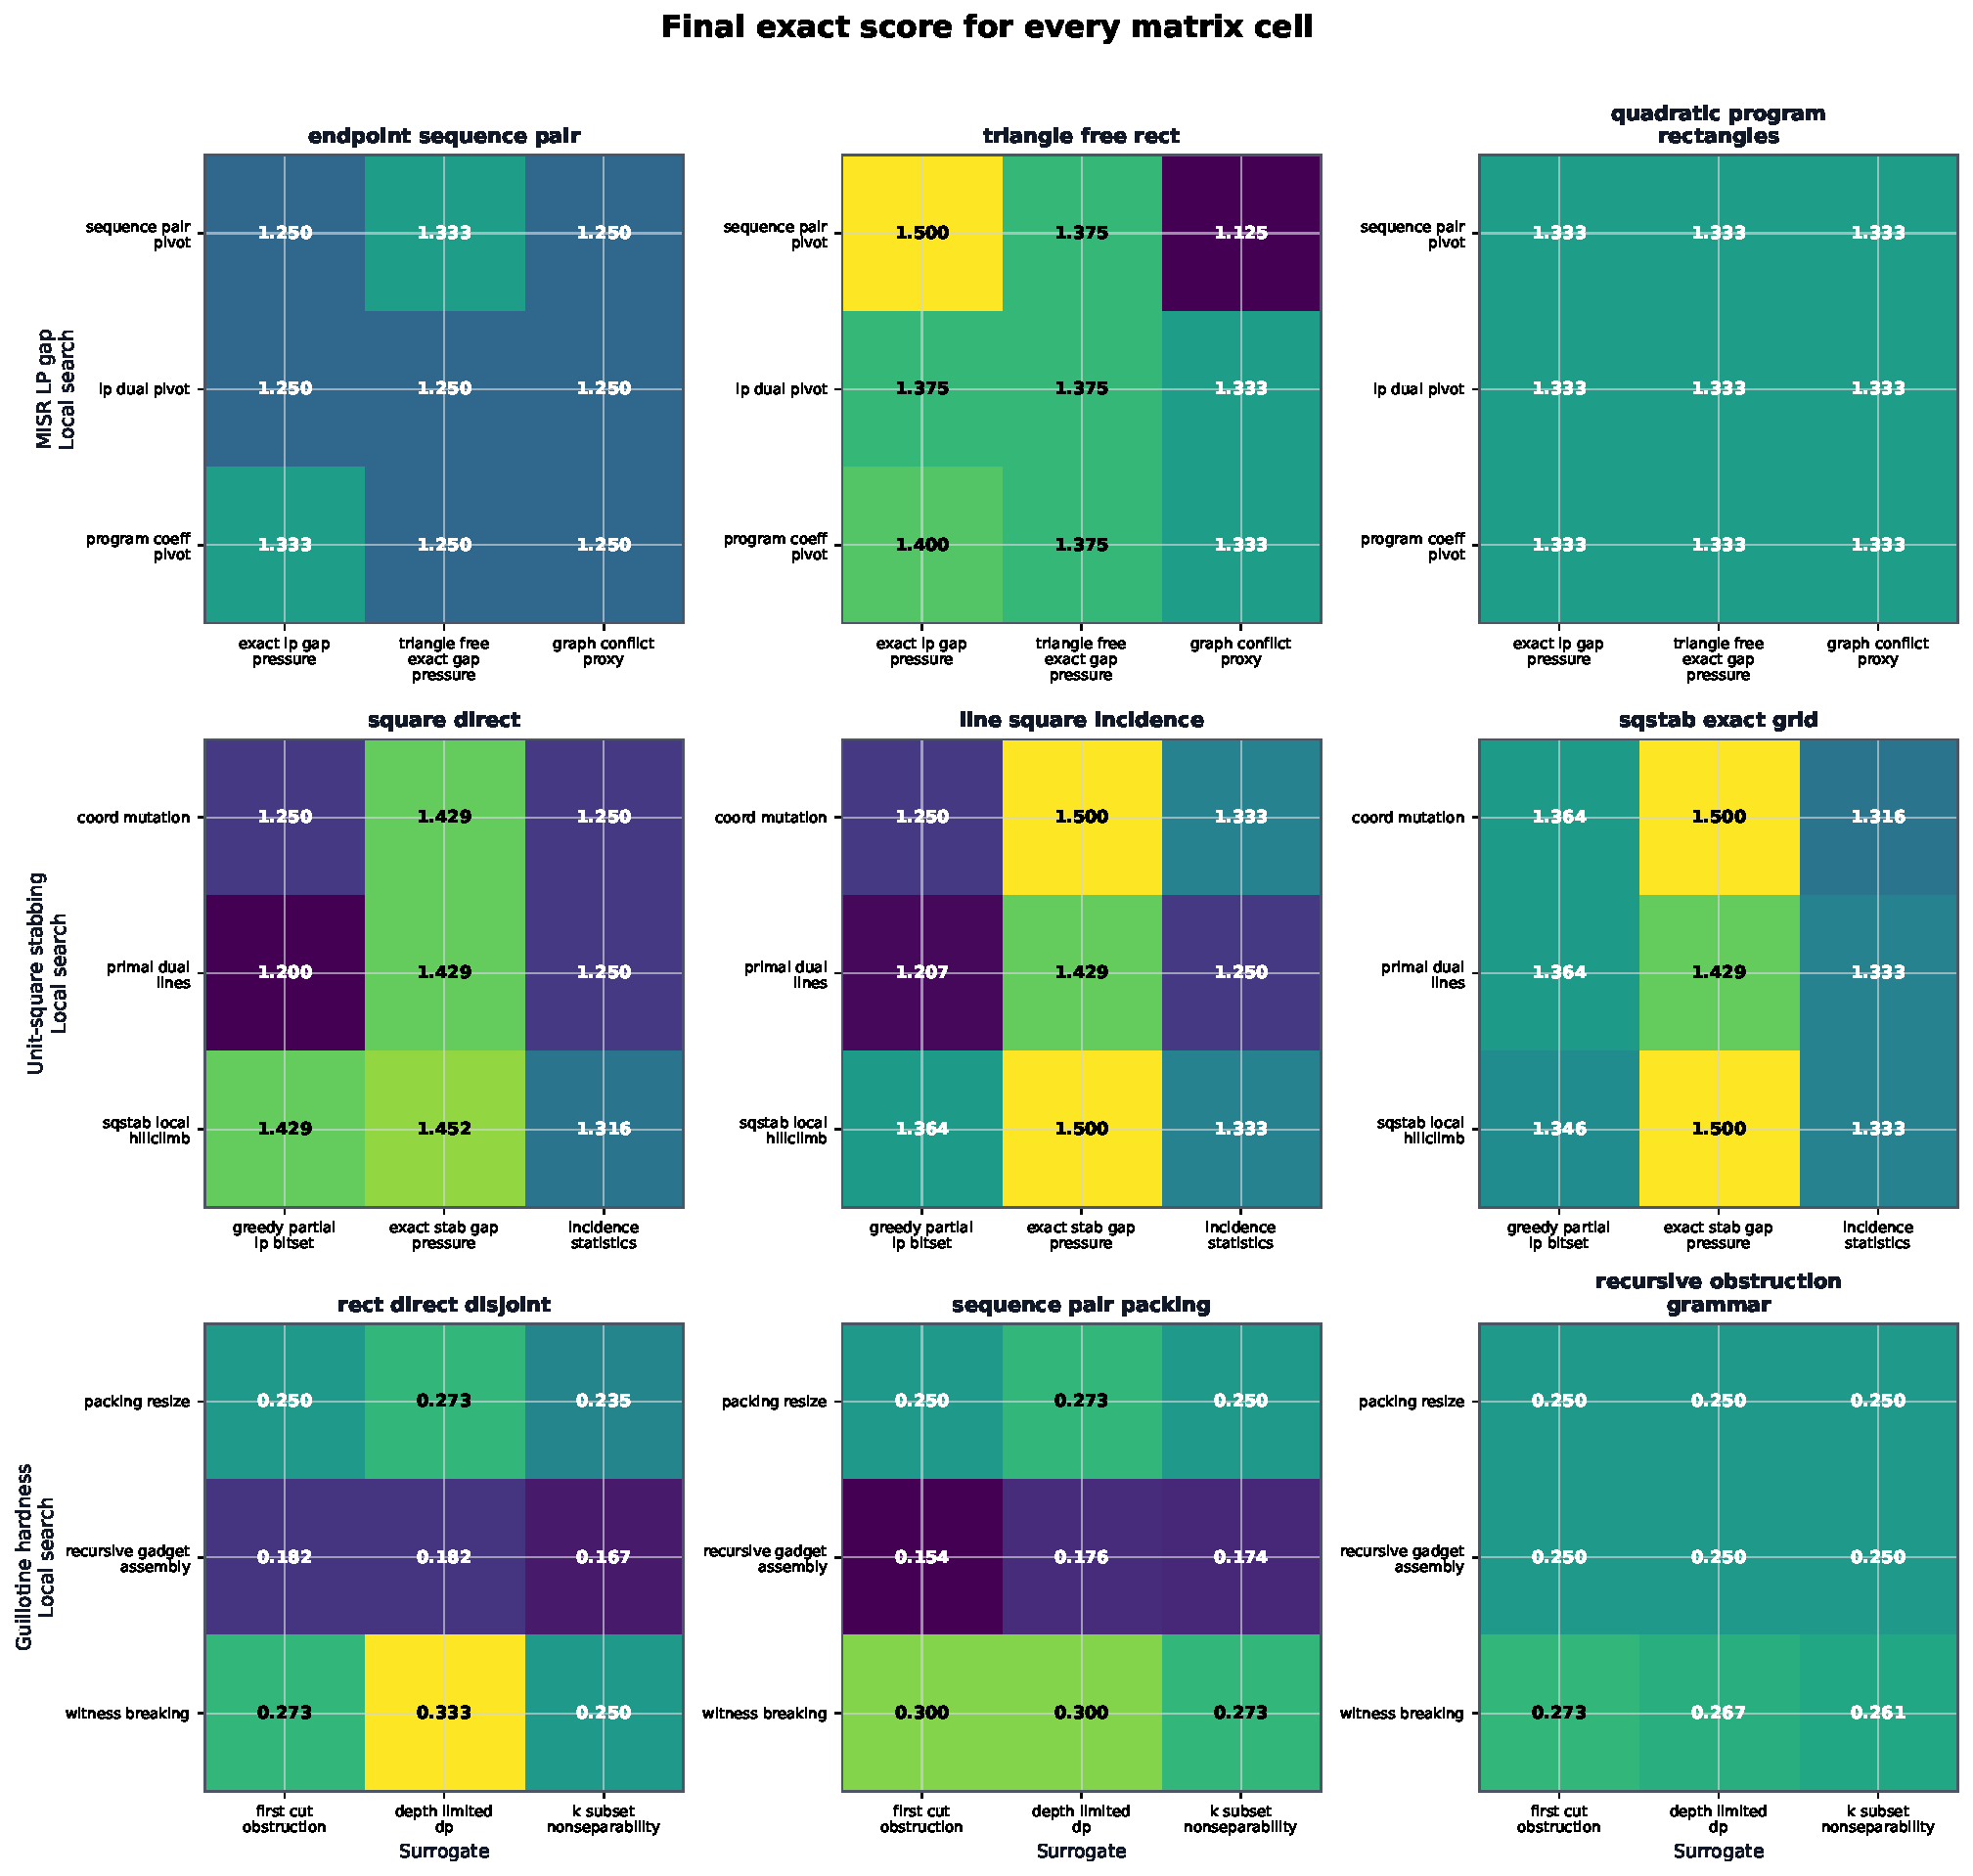
\includegraphics[width=\textwidth]{fig_final_score_heatmaps_81.pdf}
\caption{Final exact score in every cell.  Rows within each panel are local
searches, columns are surrogates, and the three panels in each problem row are
representations.  Color ranges are normalized within a problem; printed
numbers are the evidence.}
\label{fig:heatmaps}
\end{figure}

\scriptsize
\begin{longtable}{@{}p{0.08\textwidth}p{0.055\textwidth}p{0.145\textwidth}p{0.145\textwidth}p{0.145\textwidth}rrr@{}}
\caption{Top five configurations per problem. Epoch is cumulative transformer training epoch; time is elapsed hours to the first appearance of the final best.}
\label{tab:top-configs}\\
\toprule
Problem & Score & Representation & Local search & Surrogate & Epoch & Time & Items \\
\midrule
\endfirsthead
\toprule
Problem & Score & Representation & Local search & Surrogate & Epoch & Time & Items \\
\midrule
\endhead
\bottomrule
\endfoot
MISR & $\frac{3}{2}$ & \code{triangle\_\allowbreak{}free\_\allowbreak{}rect} & \code{sequence\_\allowbreak{}pair\_\allowbreak{}pivot} & \code{exact\_\allowbreak{}lp\_\allowbreak{}gap\_\allowbreak{}pressure} & 1860 & 3.12 & 12 \\
MISR & $\frac{7}{5}$ & \code{triangle\_\allowbreak{}free\_\allowbreak{}rect} & \code{program\_\allowbreak{}coeff\_\allowbreak{}pivot} & \code{exact\_\allowbreak{}lp\_\allowbreak{}gap\_\allowbreak{}pressure} & 4782 & 14.48 & 14 \\
MISR & $\frac{11}{8}$ & \code{triangle\_\allowbreak{}free\_\allowbreak{}rect} & \code{lp\_\allowbreak{}dual\_\allowbreak{}pivot} & \code{triangle\_\allowbreak{}free\_\allowbreak{}exact\_\allowbreak{}gap\_\allowbreak{}pressure} & 24 & 0.03 & 11 \\
MISR & $\frac{11}{8}$ & \code{triangle\_\allowbreak{}free\_\allowbreak{}rect} & \code{lp\_\allowbreak{}dual\_\allowbreak{}pivot} & \code{exact\_\allowbreak{}lp\_\allowbreak{}gap\_\allowbreak{}pressure} & 81 & 0.08 & 11 \\
MISR & $\frac{11}{8}$ & \code{triangle\_\allowbreak{}free\_\allowbreak{}rect} & \code{program\_\allowbreak{}coeff\_\allowbreak{}pivot} & \code{triangle\_\allowbreak{}free\_\allowbreak{}exact\_\allowbreak{}gap\_\allowbreak{}pressure} & 156 & 0.15 & 11 \\
\addlinespace
Unit-square & $\frac{3}{2}$ & \code{sqstab\_\allowbreak{}exact\_\allowbreak{}grid} & \code{coord\_\allowbreak{}mutation} & \code{exact\_\allowbreak{}stab\_\allowbreak{}gap\_\allowbreak{}pressure} & 117 & 0.35 & 14 \\
Unit-square & $\frac{3}{2}$ & \code{line\_\allowbreak{}square\_\allowbreak{}incidence} & \code{sqstab\_\allowbreak{}local\_\allowbreak{}hillclimb} & \code{exact\_\allowbreak{}stab\_\allowbreak{}gap\_\allowbreak{}pressure} & 3003 & 9.29 & 21 \\
Unit-square & $\frac{3}{2}$ & \code{line\_\allowbreak{}square\_\allowbreak{}incidence} & \code{coord\_\allowbreak{}mutation} & \code{exact\_\allowbreak{}stab\_\allowbreak{}gap\_\allowbreak{}pressure} & 3915 & 11.18 & 21 \\
Unit-square & $\frac{3}{2}$ & \code{sqstab\_\allowbreak{}exact\_\allowbreak{}grid} & \code{sqstab\_\allowbreak{}local\_\allowbreak{}hillclimb} & \code{exact\_\allowbreak{}stab\_\allowbreak{}gap\_\allowbreak{}pressure} & 375 & 0.46 & 19 \\
Unit-square & $\frac{45}{31}$ & \code{square\_\allowbreak{}direct} & \code{sqstab\_\allowbreak{}local\_\allowbreak{}hillclimb} & \code{exact\_\allowbreak{}stab\_\allowbreak{}gap\_\allowbreak{}pressure} & 2124 & 3.68 & 24 \\
\addlinespace
Guillotine & $\frac{1}{3}$ & \code{rect\_\allowbreak{}direct\_\allowbreak{}disjoint} & \code{witness\_\allowbreak{}breaking} & \code{depth\_\allowbreak{}limited\_\allowbreak{}dp} & 858 & 5.81 & 9 \\
Guillotine & $\frac{3}{10}$ & \code{sequence\_\allowbreak{}pair\_\allowbreak{}packing} & \code{witness\_\allowbreak{}breaking} & \code{depth\_\allowbreak{}limited\_\allowbreak{}dp} & 6 & 0.05 & 10 \\
Guillotine & $\frac{3}{10}$ & \code{sequence\_\allowbreak{}pair\_\allowbreak{}packing} & \code{witness\_\allowbreak{}breaking} & \code{first\_\allowbreak{}cut\_\allowbreak{}obstruction} & 669 & 3.51 & 10 \\
Guillotine & $\frac{3}{11}$ & \code{rect\_\allowbreak{}direct\_\allowbreak{}disjoint} & \code{packing\_\allowbreak{}resize} & \code{depth\_\allowbreak{}limited\_\allowbreak{}dp} & 345 & 1.92 & 11 \\
Guillotine & $\frac{3}{11}$ & \code{sequence\_\allowbreak{}pair\_\allowbreak{}packing} & \code{witness\_\allowbreak{}breaking} & \code{k\_\allowbreak{}subset\_\allowbreak{}nonseparability} & 45 & 2.12 & 22 \\
\addlinespace
\end{longtable}
\normalsize


\clearpage
\section{Learning dynamics across all 81 cells}

\subsection{Normalized model-epoch behavior}

\begin{figure}[tbp]
\centering
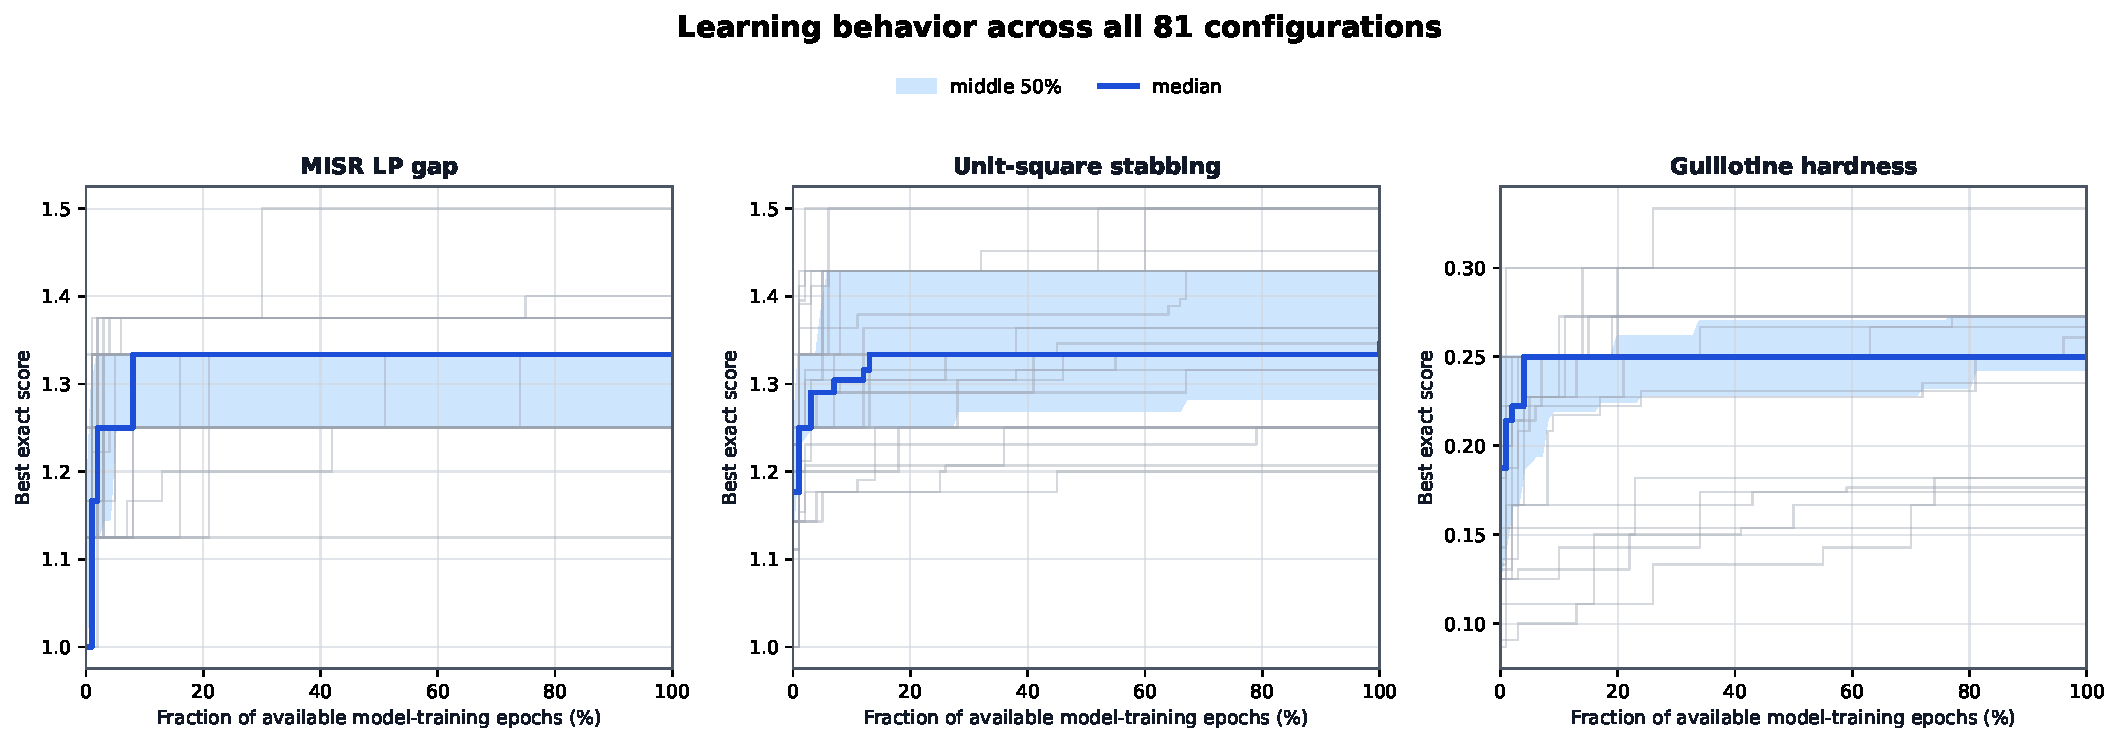
\includegraphics[width=\textwidth]{fig_all_81_normalized_epoch_curves.pdf}
\caption{All 27 trajectories per problem after normalizing each cell by its
available cumulative transformer-training epochs.  Gray lines are individual
configurations; the blue line is the median and the band is the middle 50\%.
This normalization compares the shape of learning, not raw computational
throughput.}
\label{fig:all-curves}
\end{figure}

A long horizontal segment means that additional model updates and local
search failed to improve the exact record.  A late jump can mean either that
the model found a new structural combination or that local mutation crossed a
rare discrete objective threshold.  The source analysis below separates
those cases.

\subsection{Early prediction of the final ranking}

\begin{figure}[tbp]
\centering
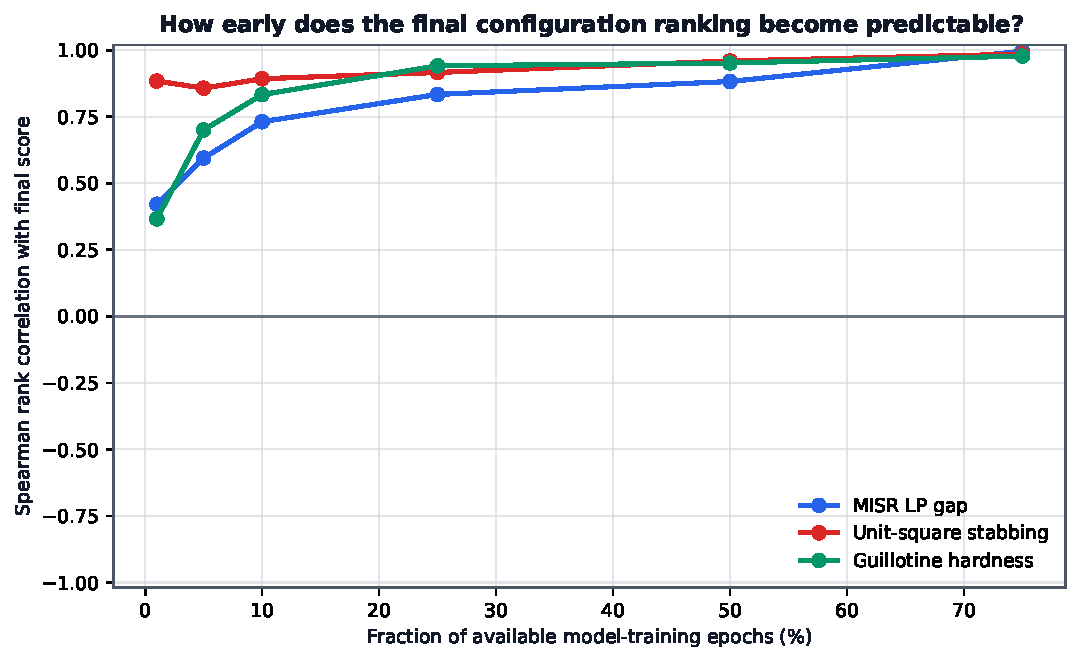
\includegraphics[width=0.82\textwidth]{fig_early_to_final_rank_stability.pdf}
\caption{Spearman rank correlation between the configuration ranking at an
early fraction of the model-epoch budget and the final ranking.  Because each
cell is a different configuration and there are no repeated seeds, the curve
is descriptive rather than an inferential test.}
\label{fig:rank-stability}
\end{figure}

At 25\% of the epoch budget, the descriptive rank correlations with the final
ranking are \MisrRankRhoTwentyFive{} for MISR,
\UnitSquareRankRhoTwentyFive{} for unit-square stabbing, and
\GuillotineRankRhoTwentyFive{} for guillotine hardness.  High early
correlation indicates that longer runtime mostly refines an ordering already
visible early; low correlation indicates meaningful late rearrangement among
configurations.

All three correlations exceed $0.83$ by this point.  Unit-square and
guillotine rankings are already strongly predictive after only 10\% of the
epoch budget, while MISR reorganizes somewhat longer.  The remaining runtime
mostly extends plateaus or improves a small number of outlying cells rather
than changing the broad component ordering.

\subsection{Where strict improvements came from}

\begin{figure}[tbp]
\centering
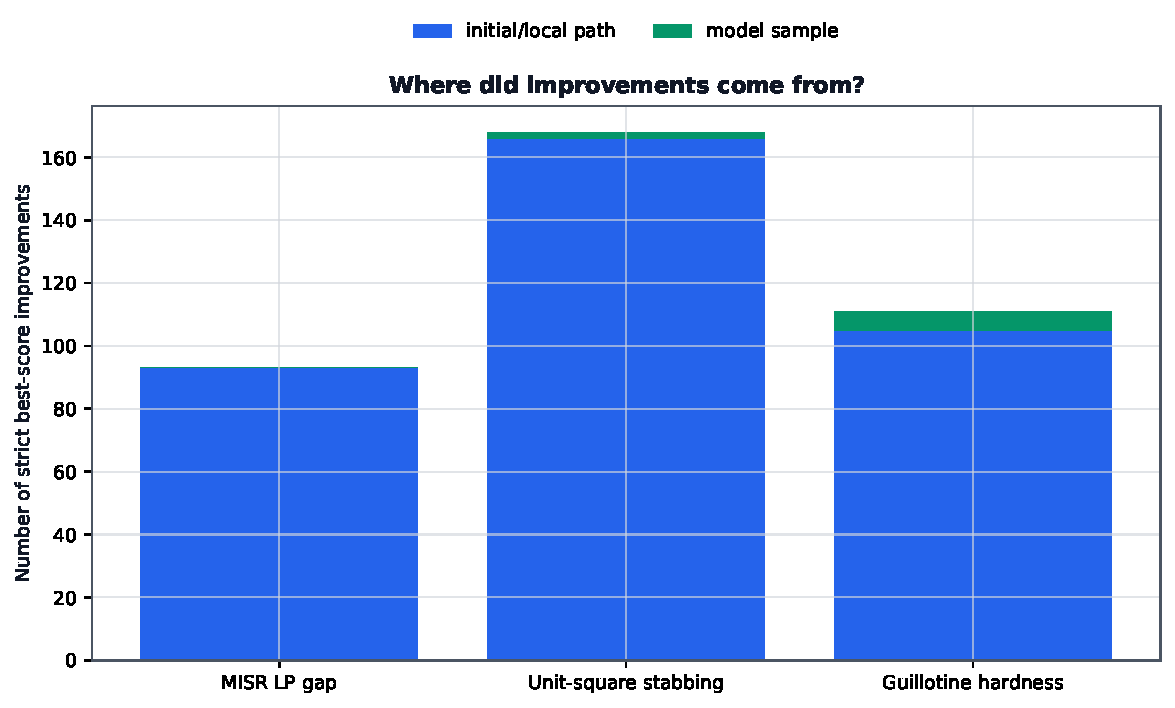
\includegraphics[width=0.84\textwidth]{fig_improvement_sources.pdf}
\caption{Source of every strict best-score improvement recorded in the 81
event streams.  A model sample is counted only when that sampled candidate is
exactly audited and strictly improves the saved record.}
\label{fig:improvement-sources}
\end{figure}

The learned-model path contributes to discovery only when it generates a
valid candidate that survives representation repair, satisfies
nontriviality, and beats the exact incumbent.  The event schema labels these
candidates \code{model\_sample}; it does not distinguish a direct transformer
sample from an n-gram backfill.  The corresponding fractions of all strict
improvements are \MisrModelImprovementPercent\%,
\UnitSquareModelImprovementPercent\%, and
\GuillotineModelImprovementPercent\%.  This statistic is more informative
than the raw number of training calls: a model can train thousands of times
while mostly reproducing the archive or proposing invalid candidates.
In absolute terms, the event streams contain no model-sourced strict MISR
improvement, only two for unit-square stabbing, and six for guillotine.  The
combined initialization/local-mutation path accounts for 93, 166, and 105
strict improvements, respectively.  The combined label is deliberate:
code{initial\_or\_local} events do not support a finer attribution.

\subsection{Plateaus and computational throughput}

\begin{figure}[tbp]
\centering
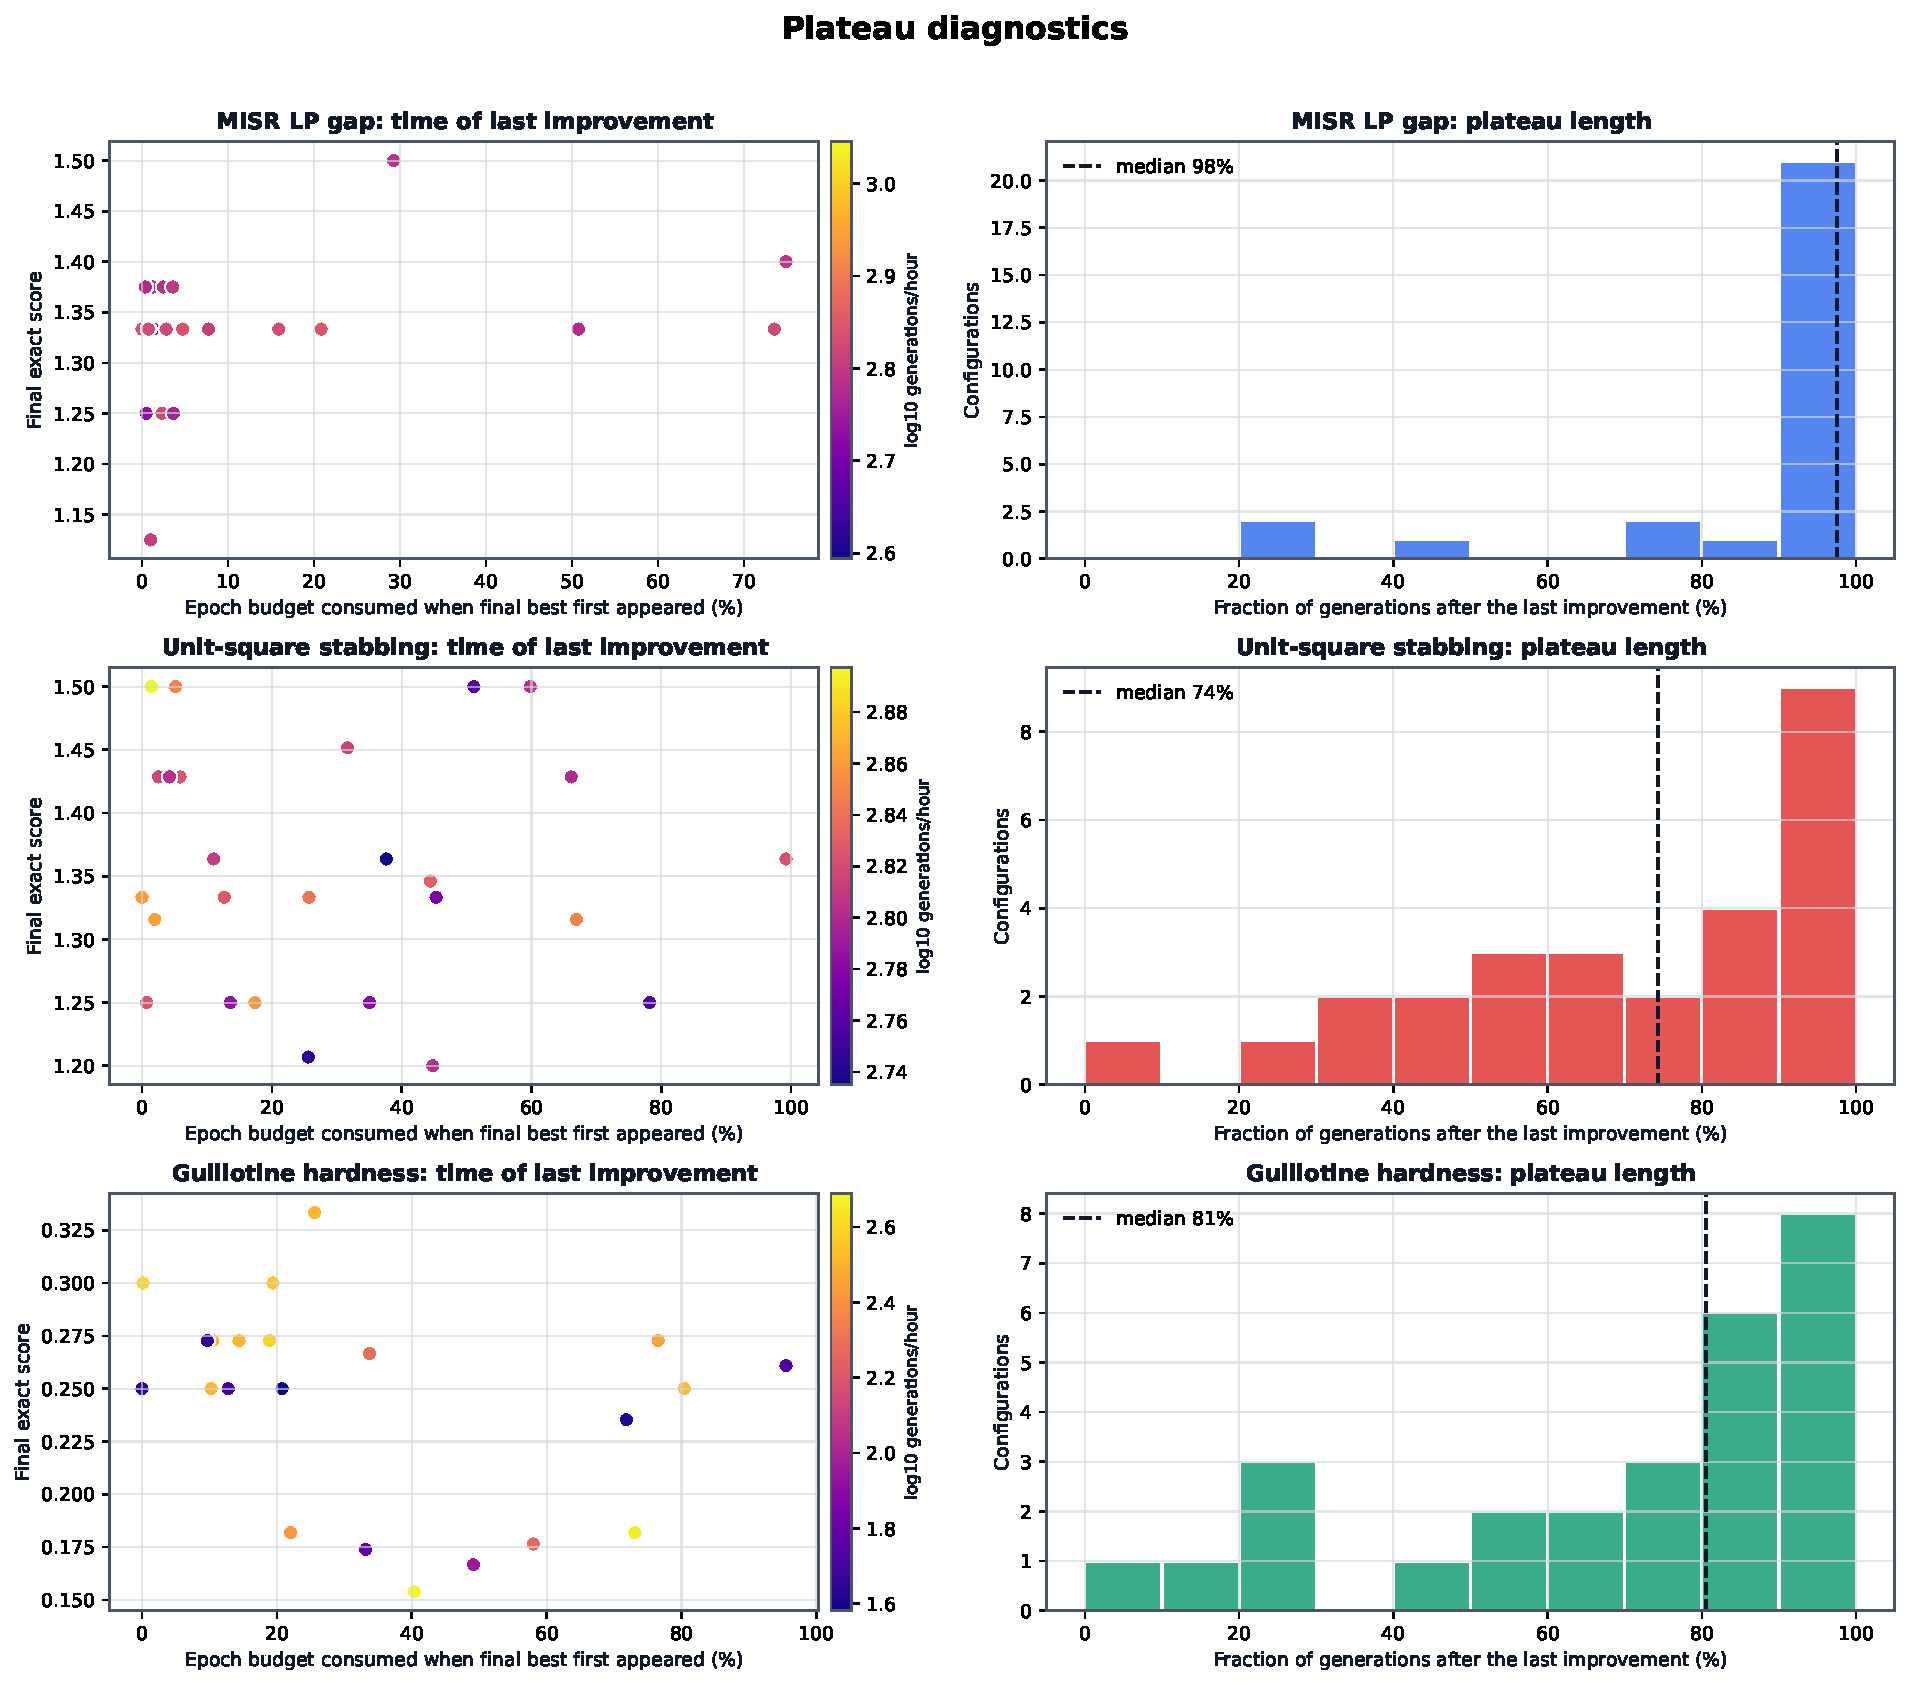
\includegraphics[width=\textwidth]{fig_plateau_diagnostics.pdf}
\caption{Left: when each cell first reached its final score, colored by search
throughput.  Right: fraction of search generations after the final strict
improvement.  Long plateaus provide direct evidence that wall time alone was
not the principal missing ingredient.}
\label{fig:plateaus}
\end{figure}

The median post-best plateau occupies \MisrMedianPlateauPercent\% of MISR
generations, \UnitSquareMedianPlateauPercent\% of unit-square generations,
and \GuillotineMedianPlateauPercent\% of guillotine generations.  The top
records first appeared after \MisrTopTimeToBestHours{},
\UnitSquareTopTimeToBestHours{}, and \GuillotineTopTimeToBestHours{} hours.

\begin{figure}[tbp]
\centering
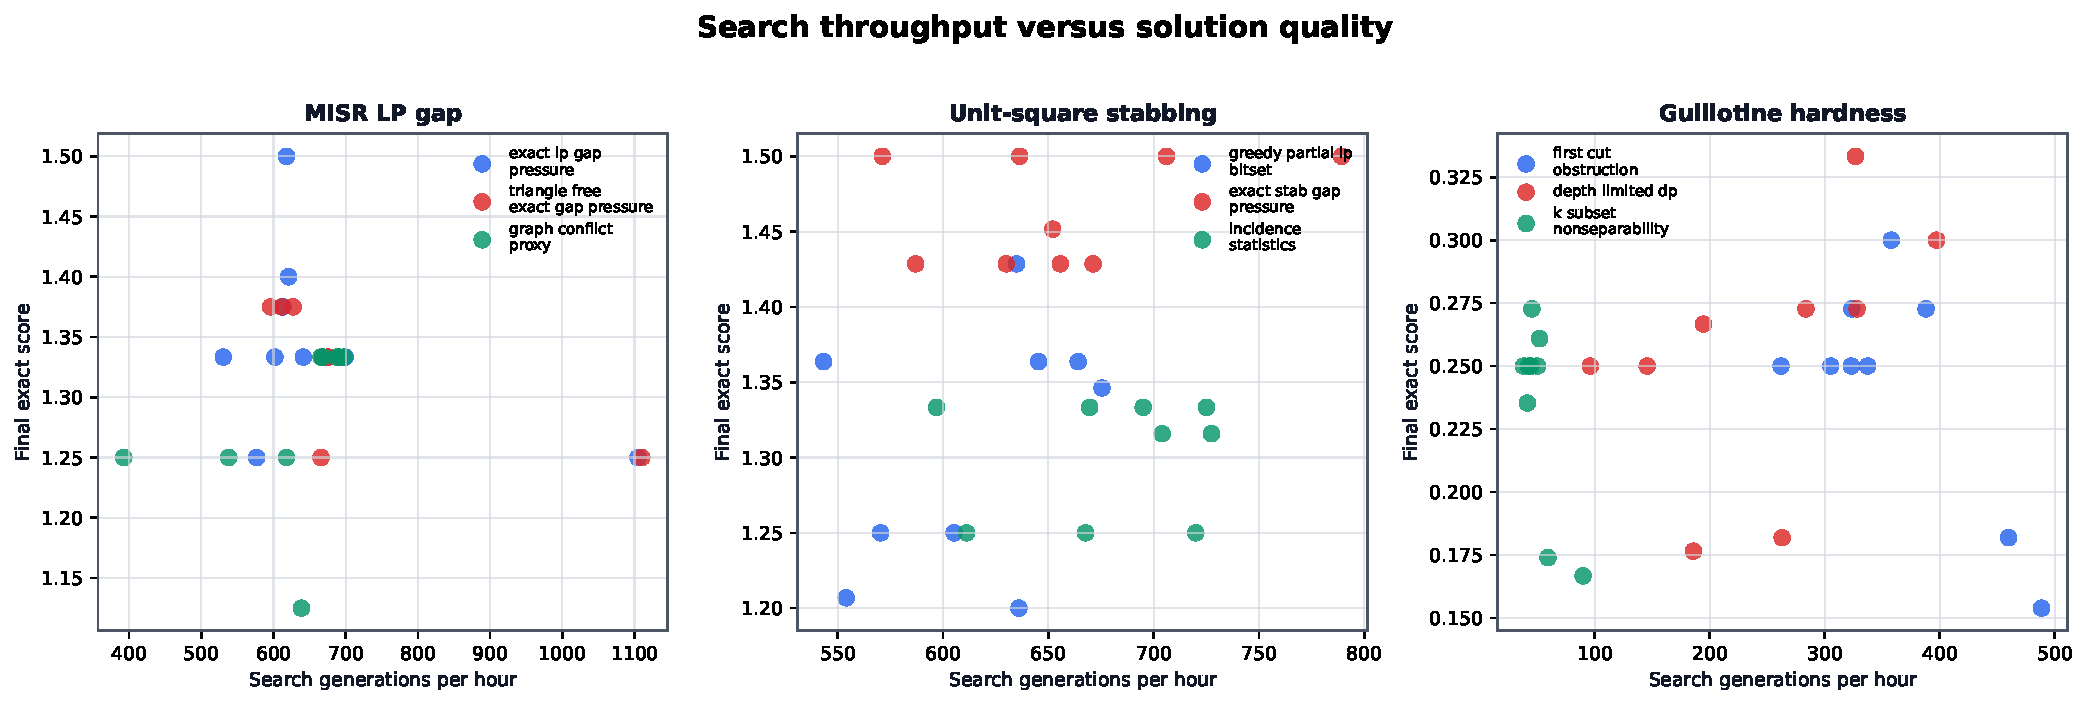
\includegraphics[width=\textwidth]{fig_throughput_vs_quality.pdf}
\caption{Search generations completed per hour versus final exact score.
Exact or deeper surrogates may lower throughput while improving alignment;
fast proxies are useful only if their additional generations translate into
better exact certificates.}
\label{fig:throughput}
\end{figure}

\begin{figure}[tbp]
\centering
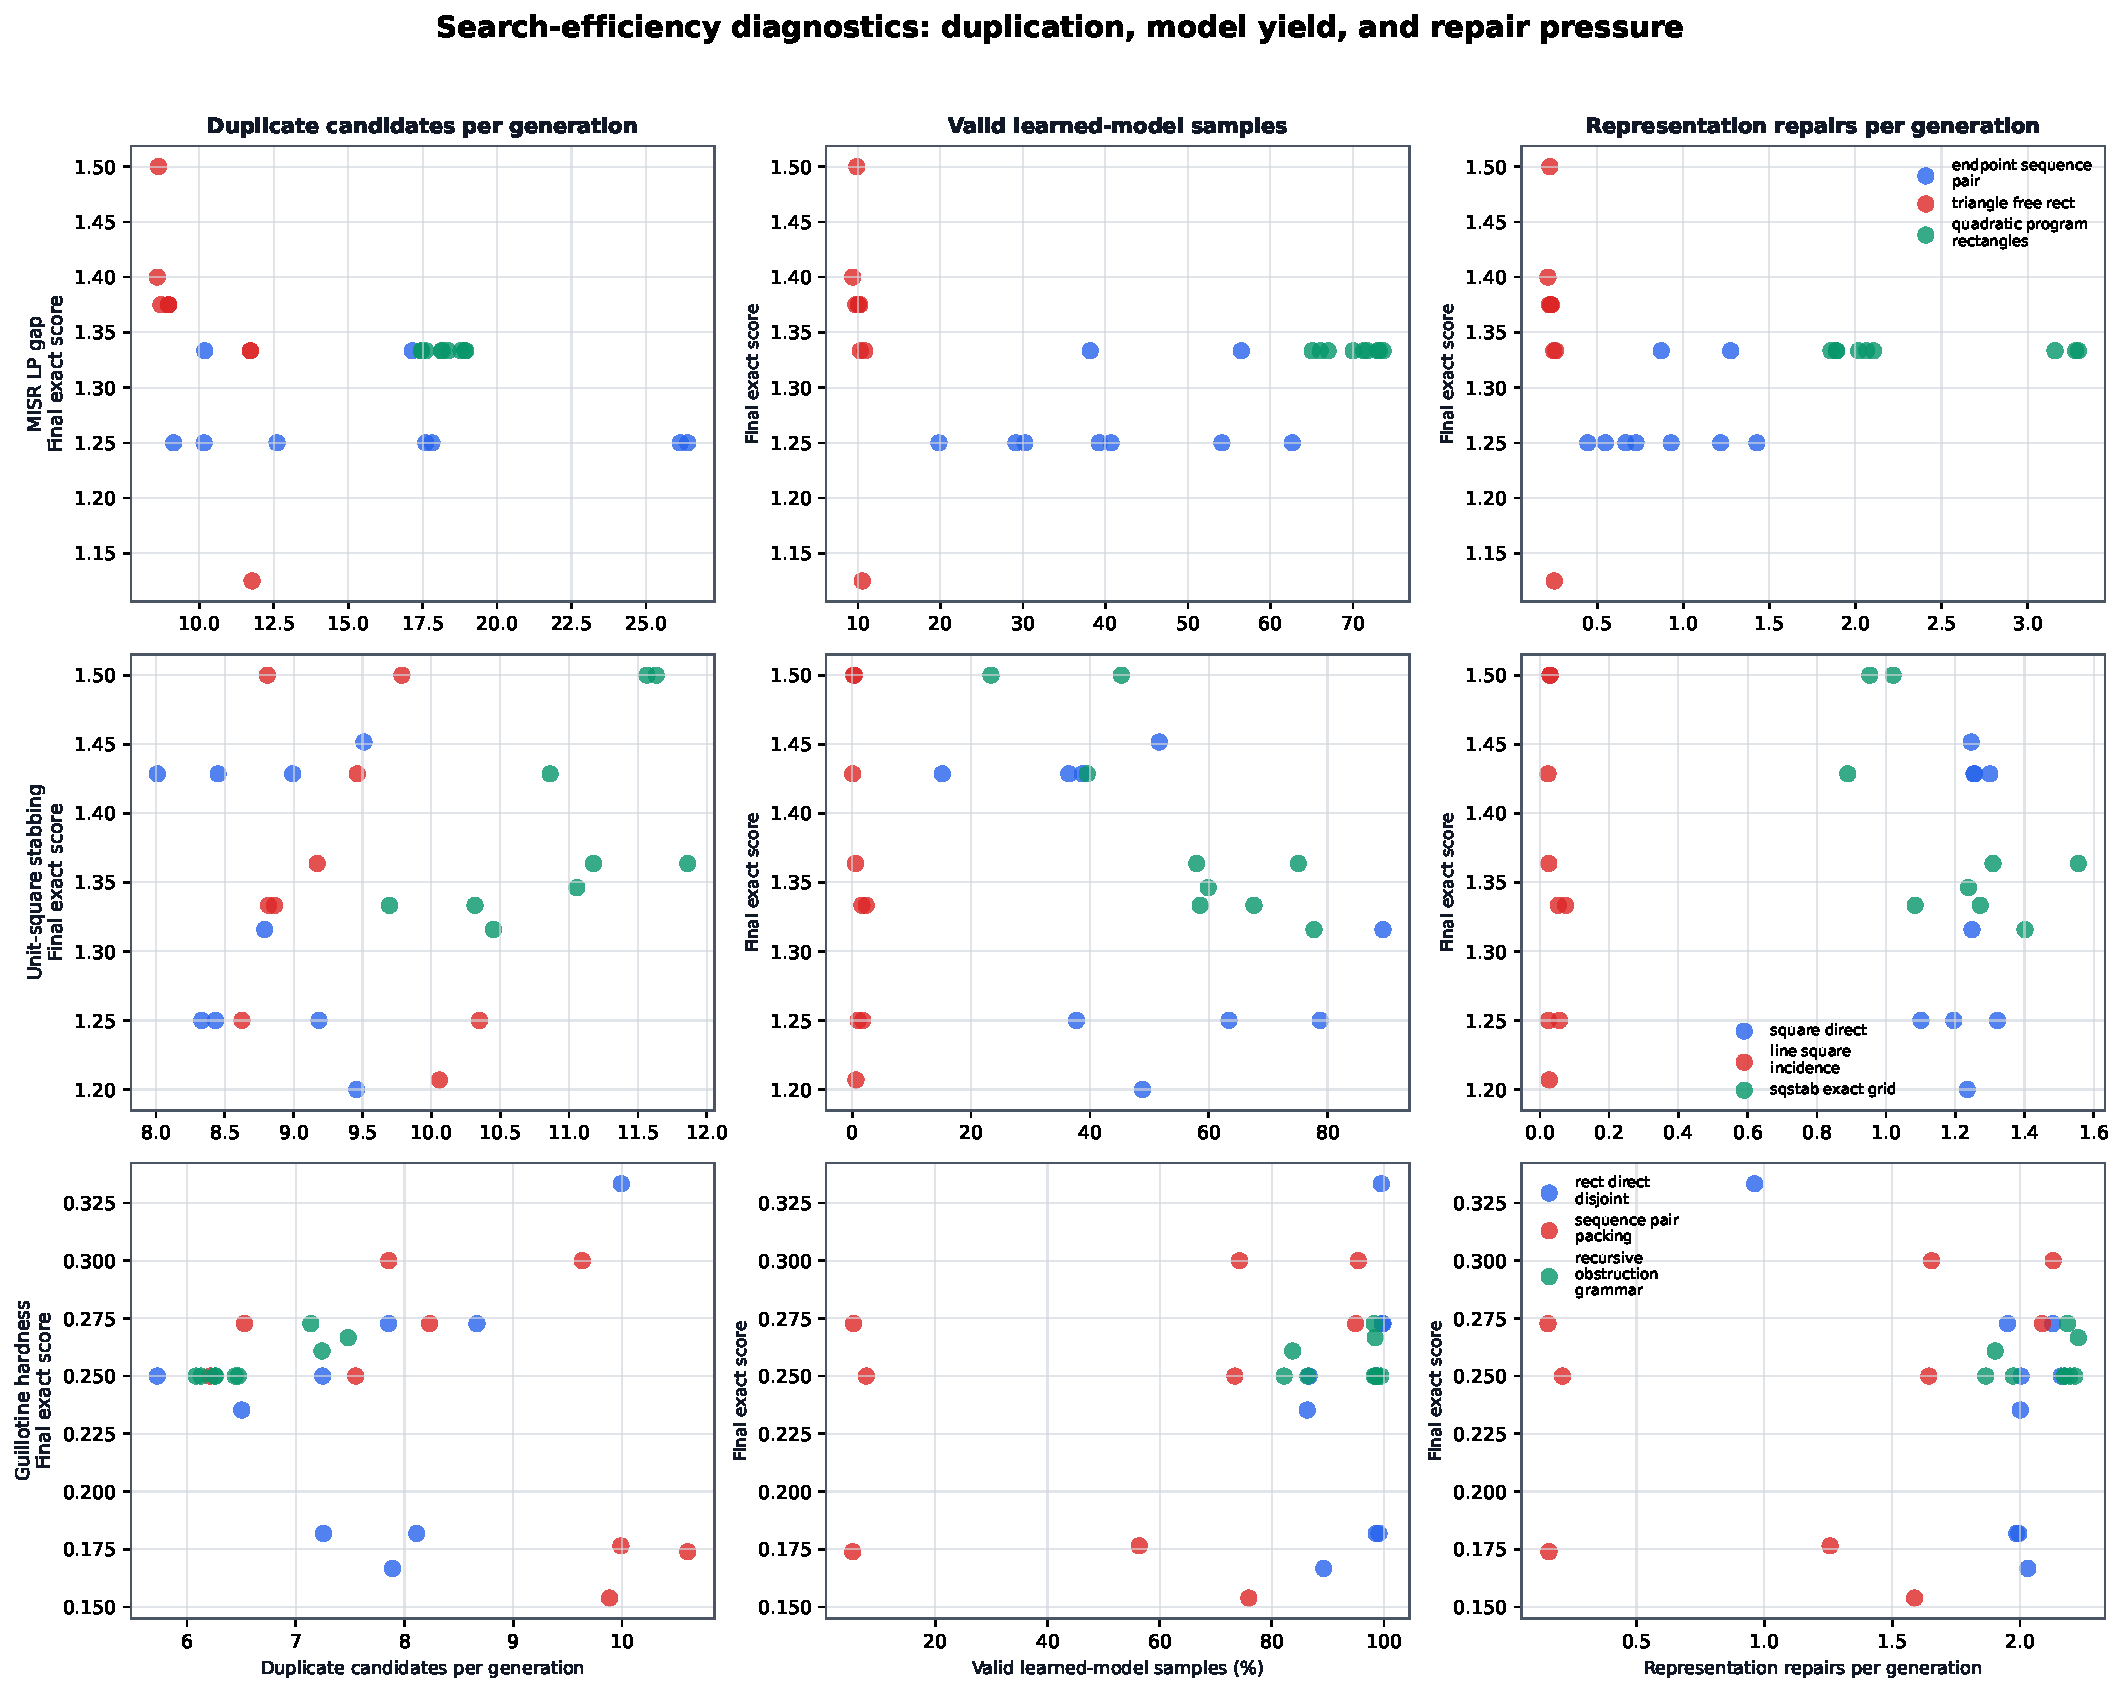
\includegraphics[width=\textwidth]{fig_search_efficiency_diagnostics.pdf}
\caption{Final score against duplicate pressure, valid learned-model sample
yield, and representation-repair pressure.  These diagnostics test whether
additional training produces genuinely new feasible structures or repeatedly
returns to the same basin.}
\label{fig:search-efficiency}
\end{figure}

The median cell produced \MisrMedianDuplicatesPerGeneration{} duplicate
candidates per MISR generation, \UnitSquareMedianDuplicatesPerGeneration{}
per unit-square generation, and \GuillotineMedianDuplicatesPerGeneration{}
per guillotine generation, from a population of 32.  Median valid
learned-model yields were only \MisrMedianModelValidPercent\% and
\UnitSquareMedianModelValidPercent\% for the two LP-gap problems, versus
\GuillotineMedianModelValidPercent\% for guillotine.  High syntactic validity
therefore does not imply useful novelty: guillotine proposals were often
repairable, yet their exact scores still plateaued.

\clearpage
\section{Problem 1: MISR LP-gap search}

\subsection{Objective and exact verifier}

For a finite family $\Rcal$ of axis-parallel rectangles, the exact score is
\[
  \score_{\mathrm{MISR}}(\Rcal)
  =\frac{\alpha^*(\Rcal)}{\alpha(\Rcal)},
\]
where $\alpha$ is the maximum number of pairwise-disjoint rectangles and
$\alpha^*$ is the clique-LP optimum of the rectangle intersection graph.  The
certificate stores all rectangles, the intersection graph, maximal cliques,
an optimal integral independent set, LP primal and dual values, and solver
status.  The verifier reconstructs and solves both optimization problems.

\subsection{All 27 trajectories}

\begin{figure}[p]
\centering
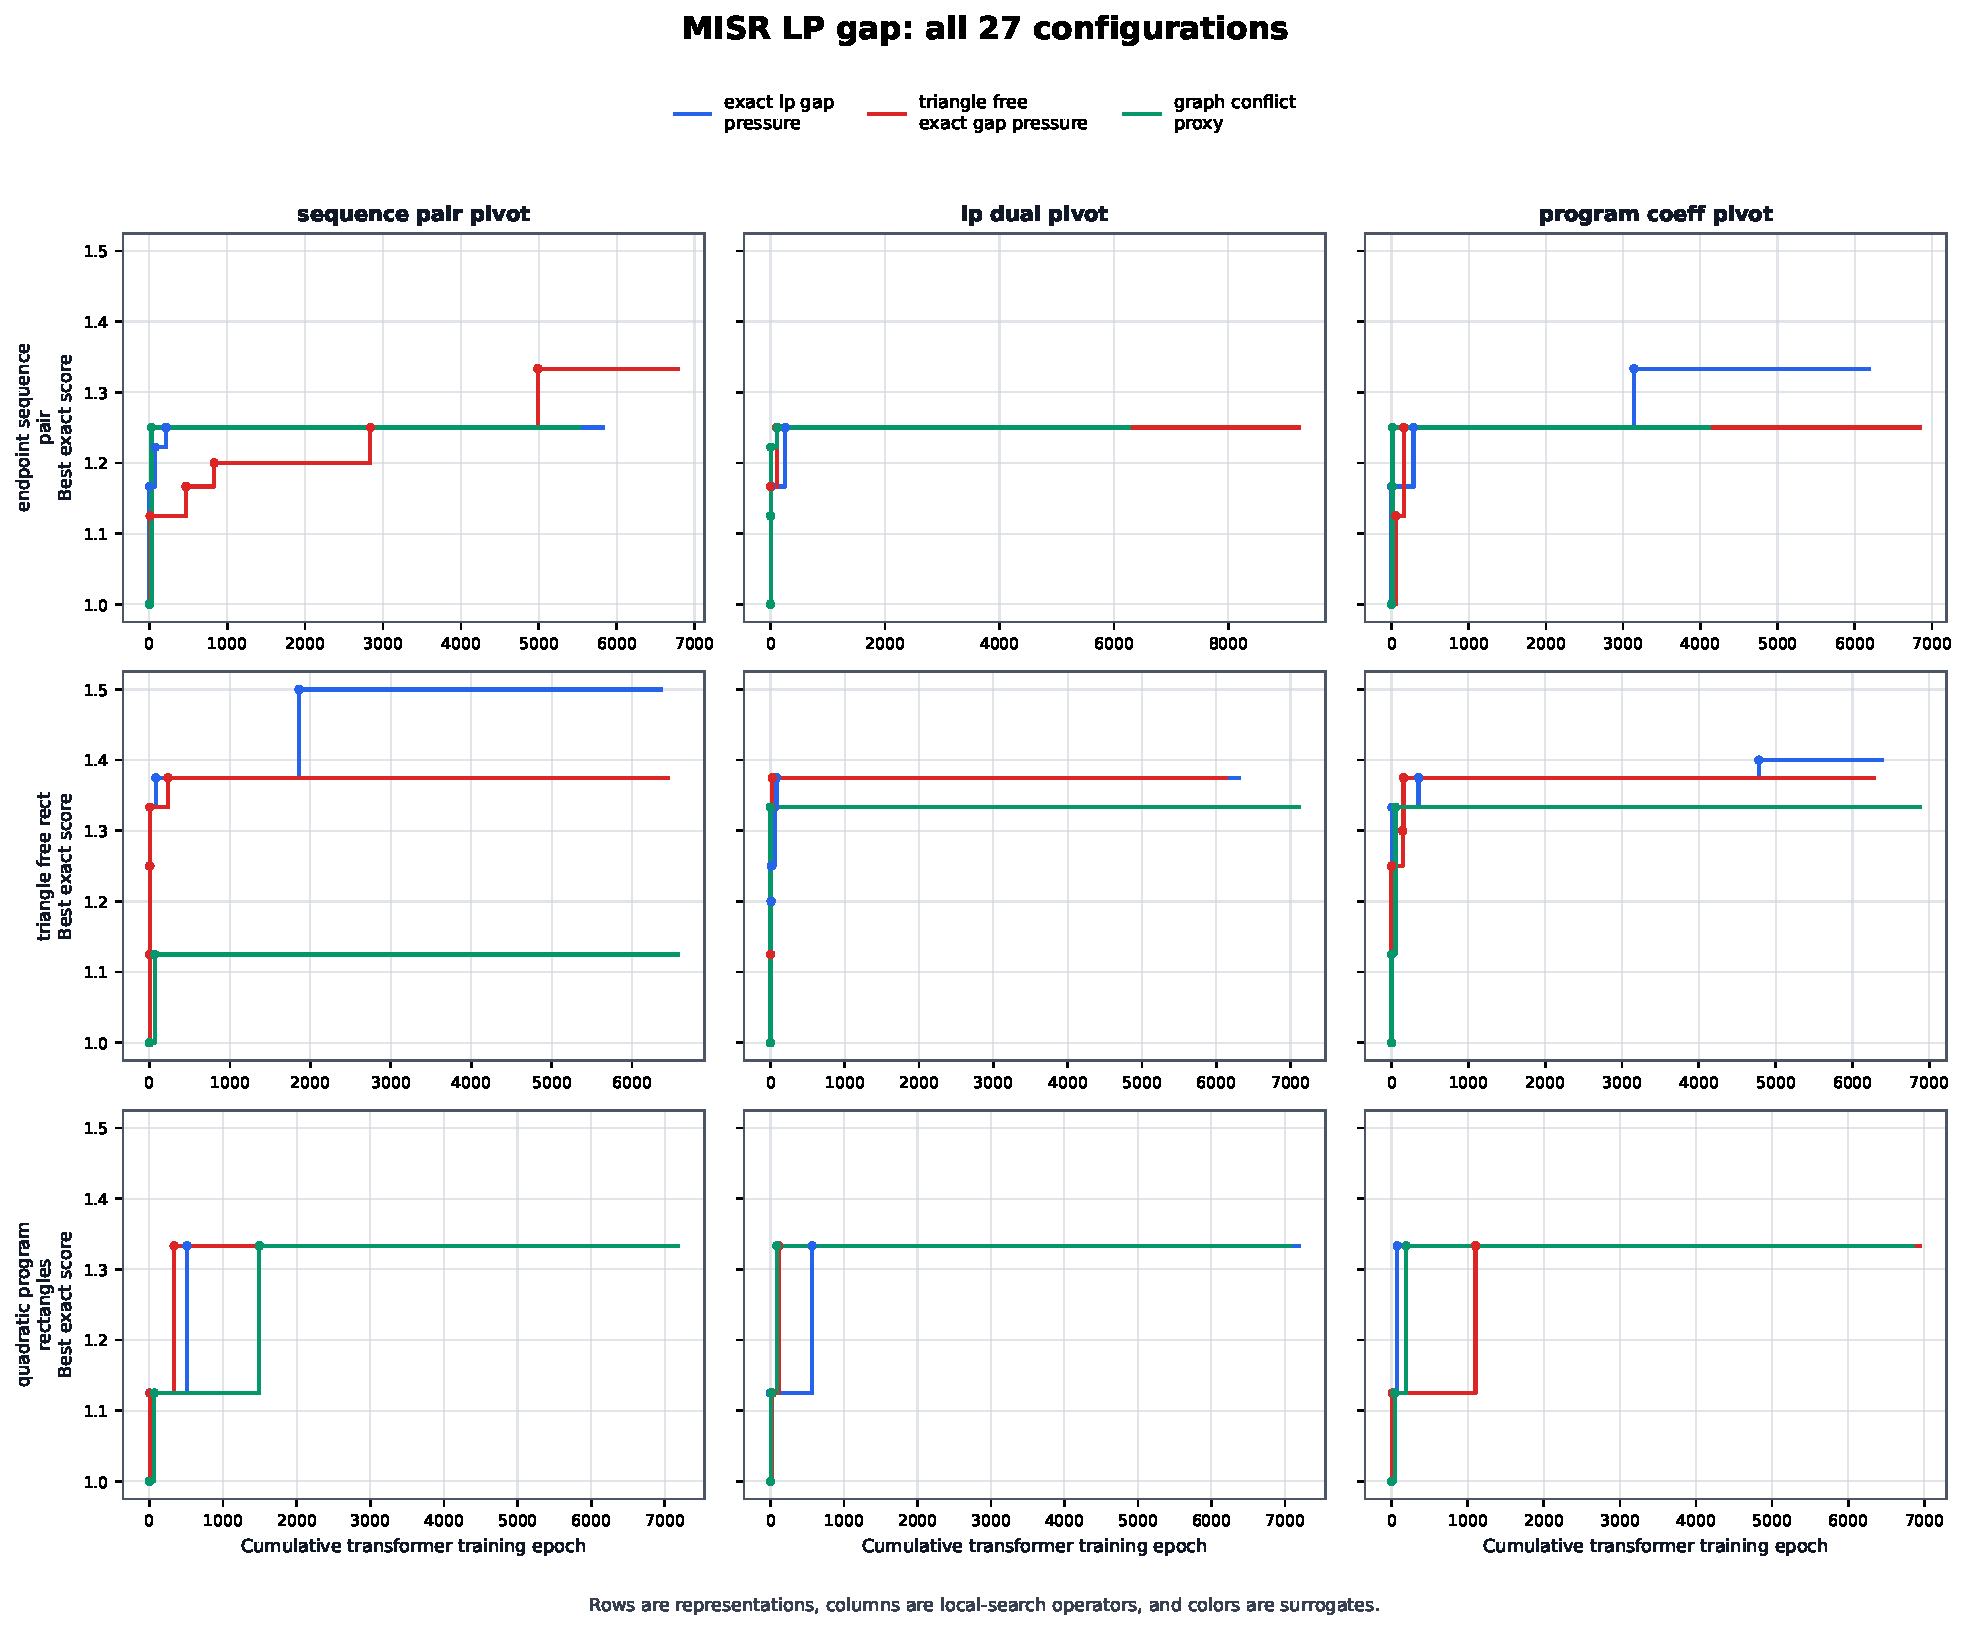
\includegraphics[width=\textwidth]{fig_misr_27_trajectories_model_epoch.pdf}
\caption{MISR trajectories against cumulative transformer-training epoch.
Each panel fixes a representation and local search; its three colored curves
are the surrogates.}
\label{fig:misr-epochs}
\end{figure}

\begin{figure}[p]
\centering
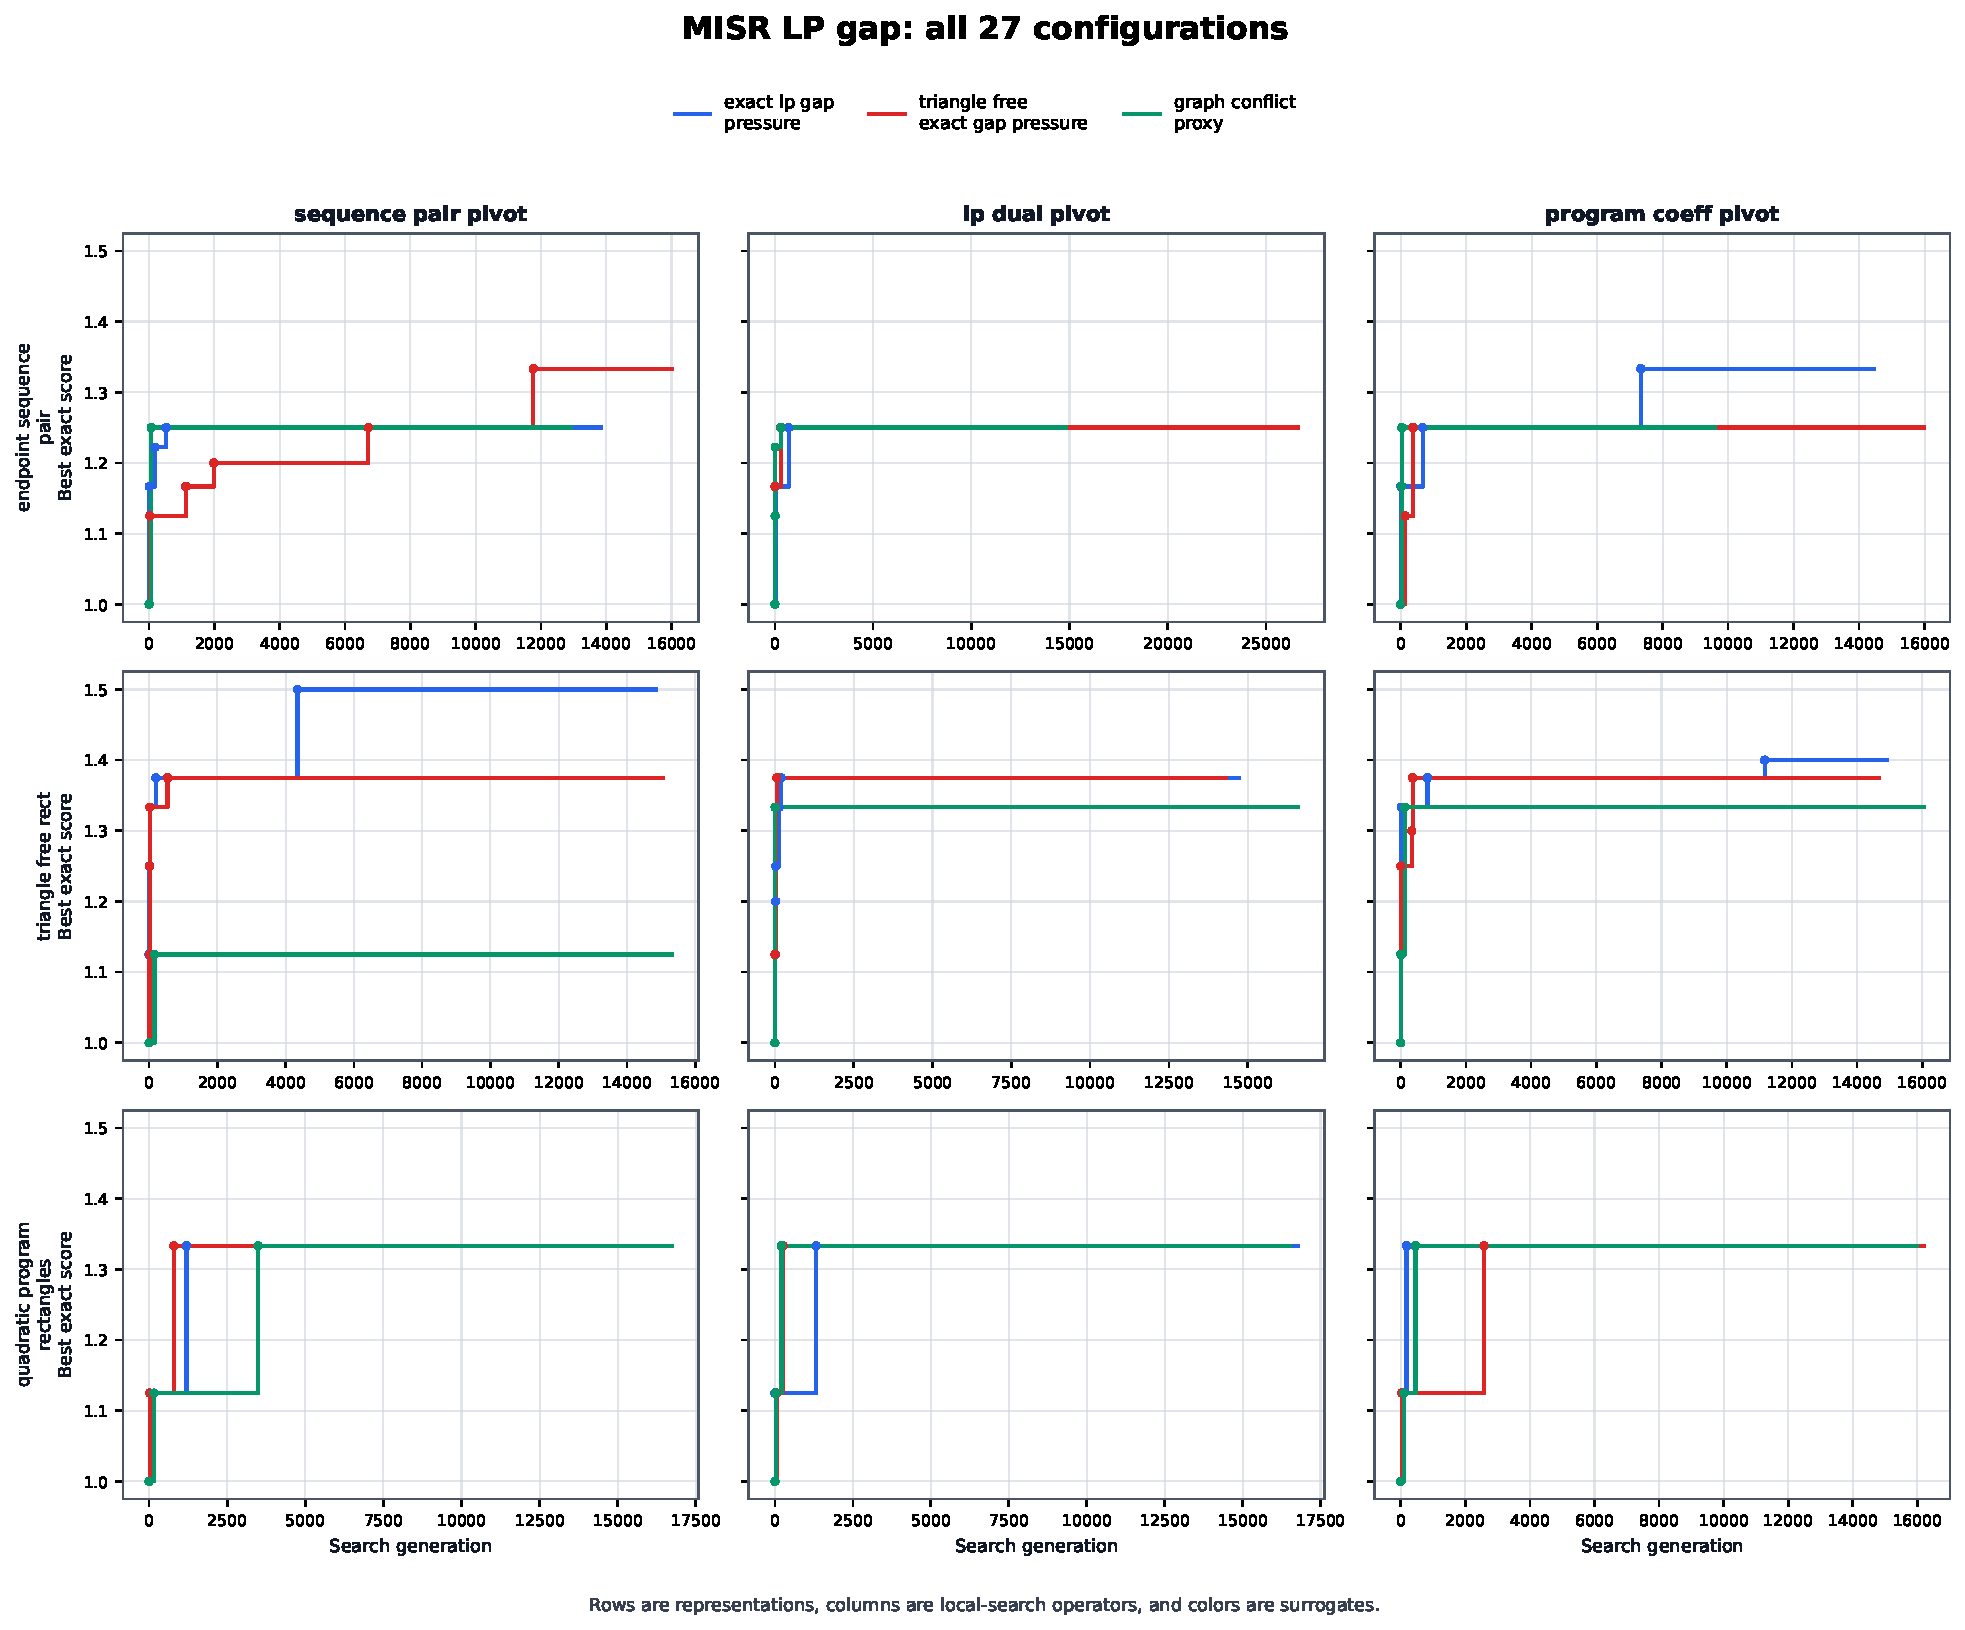
\includegraphics[width=\textwidth]{fig_misr_27_trajectories_generation.pdf}
\caption{The same 27 MISR cells against search generation.  Comparing this
figure with Figure~\ref{fig:misr-epochs} separates model-update effects from
raw local-search progress.}
\label{fig:misr-generations}
\end{figure}

\begin{table}[tbp]
\centering
\caption{Descriptive component marginals for MISR. Each level pools nine distinct component cells.}
\label{tab:misr-marginals}
\begin{tabularx}{\textwidth}{p{0.16\textwidth}Xrrrrr}
\toprule
Factor & Level & Mean & Median & Min. & Max. & IQR \\
\midrule
Representation & \code{triangle\_\allowbreak{}free\_\allowbreak{}rect} & 1.3546 & 1.3750 & 1.1250 & 1.5000 & [1.3333, 1.3750] \\
 & \code{quadratic\_\allowbreak{}program\_\allowbreak{}rectangles} & 1.3333 & 1.3333 & 1.3333 & 1.3333 & [1.3333, 1.3333] \\
 & \code{endpoint\_\allowbreak{}sequence\_\allowbreak{}pair} & 1.2685 & 1.2500 & 1.2500 & 1.3333 & [1.2500, 1.2500] \\
\addlinespace
Local Search & \code{program\_\allowbreak{}coeff\_\allowbreak{}pivot} & 1.3269 & 1.3333 & 1.2500 & 1.4000 & [1.3333, 1.3333] \\
 & \code{lp\_\allowbreak{}dual\_\allowbreak{}pivot} & 1.3148 & 1.3333 & 1.2500 & 1.3750 & [1.2500, 1.3333] \\
 & \code{sequence\_\allowbreak{}pair\_\allowbreak{}pivot} & 1.3148 & 1.3333 & 1.1250 & 1.5000 & [1.2500, 1.3333] \\
\addlinespace
Surrogate & \code{exact\_\allowbreak{}lp\_\allowbreak{}gap\_\allowbreak{}pressure} & 1.3454 & 1.3333 & 1.2500 & 1.5000 & [1.3333, 1.3750] \\
 & \code{triangle\_\allowbreak{}free\_\allowbreak{}exact\_\allowbreak{}gap\_\allowbreak{}pressure} & 1.3287 & 1.3333 & 1.2500 & 1.3750 & [1.3333, 1.3750] \\
 & \code{graph\_\allowbreak{}conflict\_\allowbreak{}proxy} & 1.2824 & 1.3333 & 1.1250 & 1.3333 & [1.2500, 1.3333] \\
\addlinespace
\bottomrule
\end{tabularx}
\end{table}


The matrix separates the effects cleanly at a descriptive level.  The
\code{triangle\_free\_rect} representation has mean score $1.3546$ and is the
only representation to reach $1.5$.  Every
\code{quadratic\_program\_rectangles} cell ends at exactly $4/3$, a striking
sign that its decoder and triangle-free repair map many different component
choices into the same objective basin.  The unrestricted endpoint-sequence
representation averages only $1.2685$.  Surrogate alignment is also visible:
\code{exact\_lp\_gap\_pressure} averages $1.3454$, compared with $1.2824$ for
\code{graph\_conflict\_proxy}.  By contrast, the three local-search marginal
means differ by only about $0.012$, so representation and scoring dominate the
choice of mutation label in this run.

\subsection{What worked}

The strongest MISR behavior combines a representation that can maintain
sparse conflict structure with a surrogate that observes the exact LP/integer
imbalance.  Triangle-free repair removes three-way cliques, making edge
constraints the clique LP and exposing half-integral pressure.  Endpoint
sequence pairs provide large combinatorial moves without tying the search to
small coordinate perturbations.  LP-aware pivots are useful when they change
tight constraints without simultaneously increasing the integral optimum.

\begin{figure}[tbp]
\centering
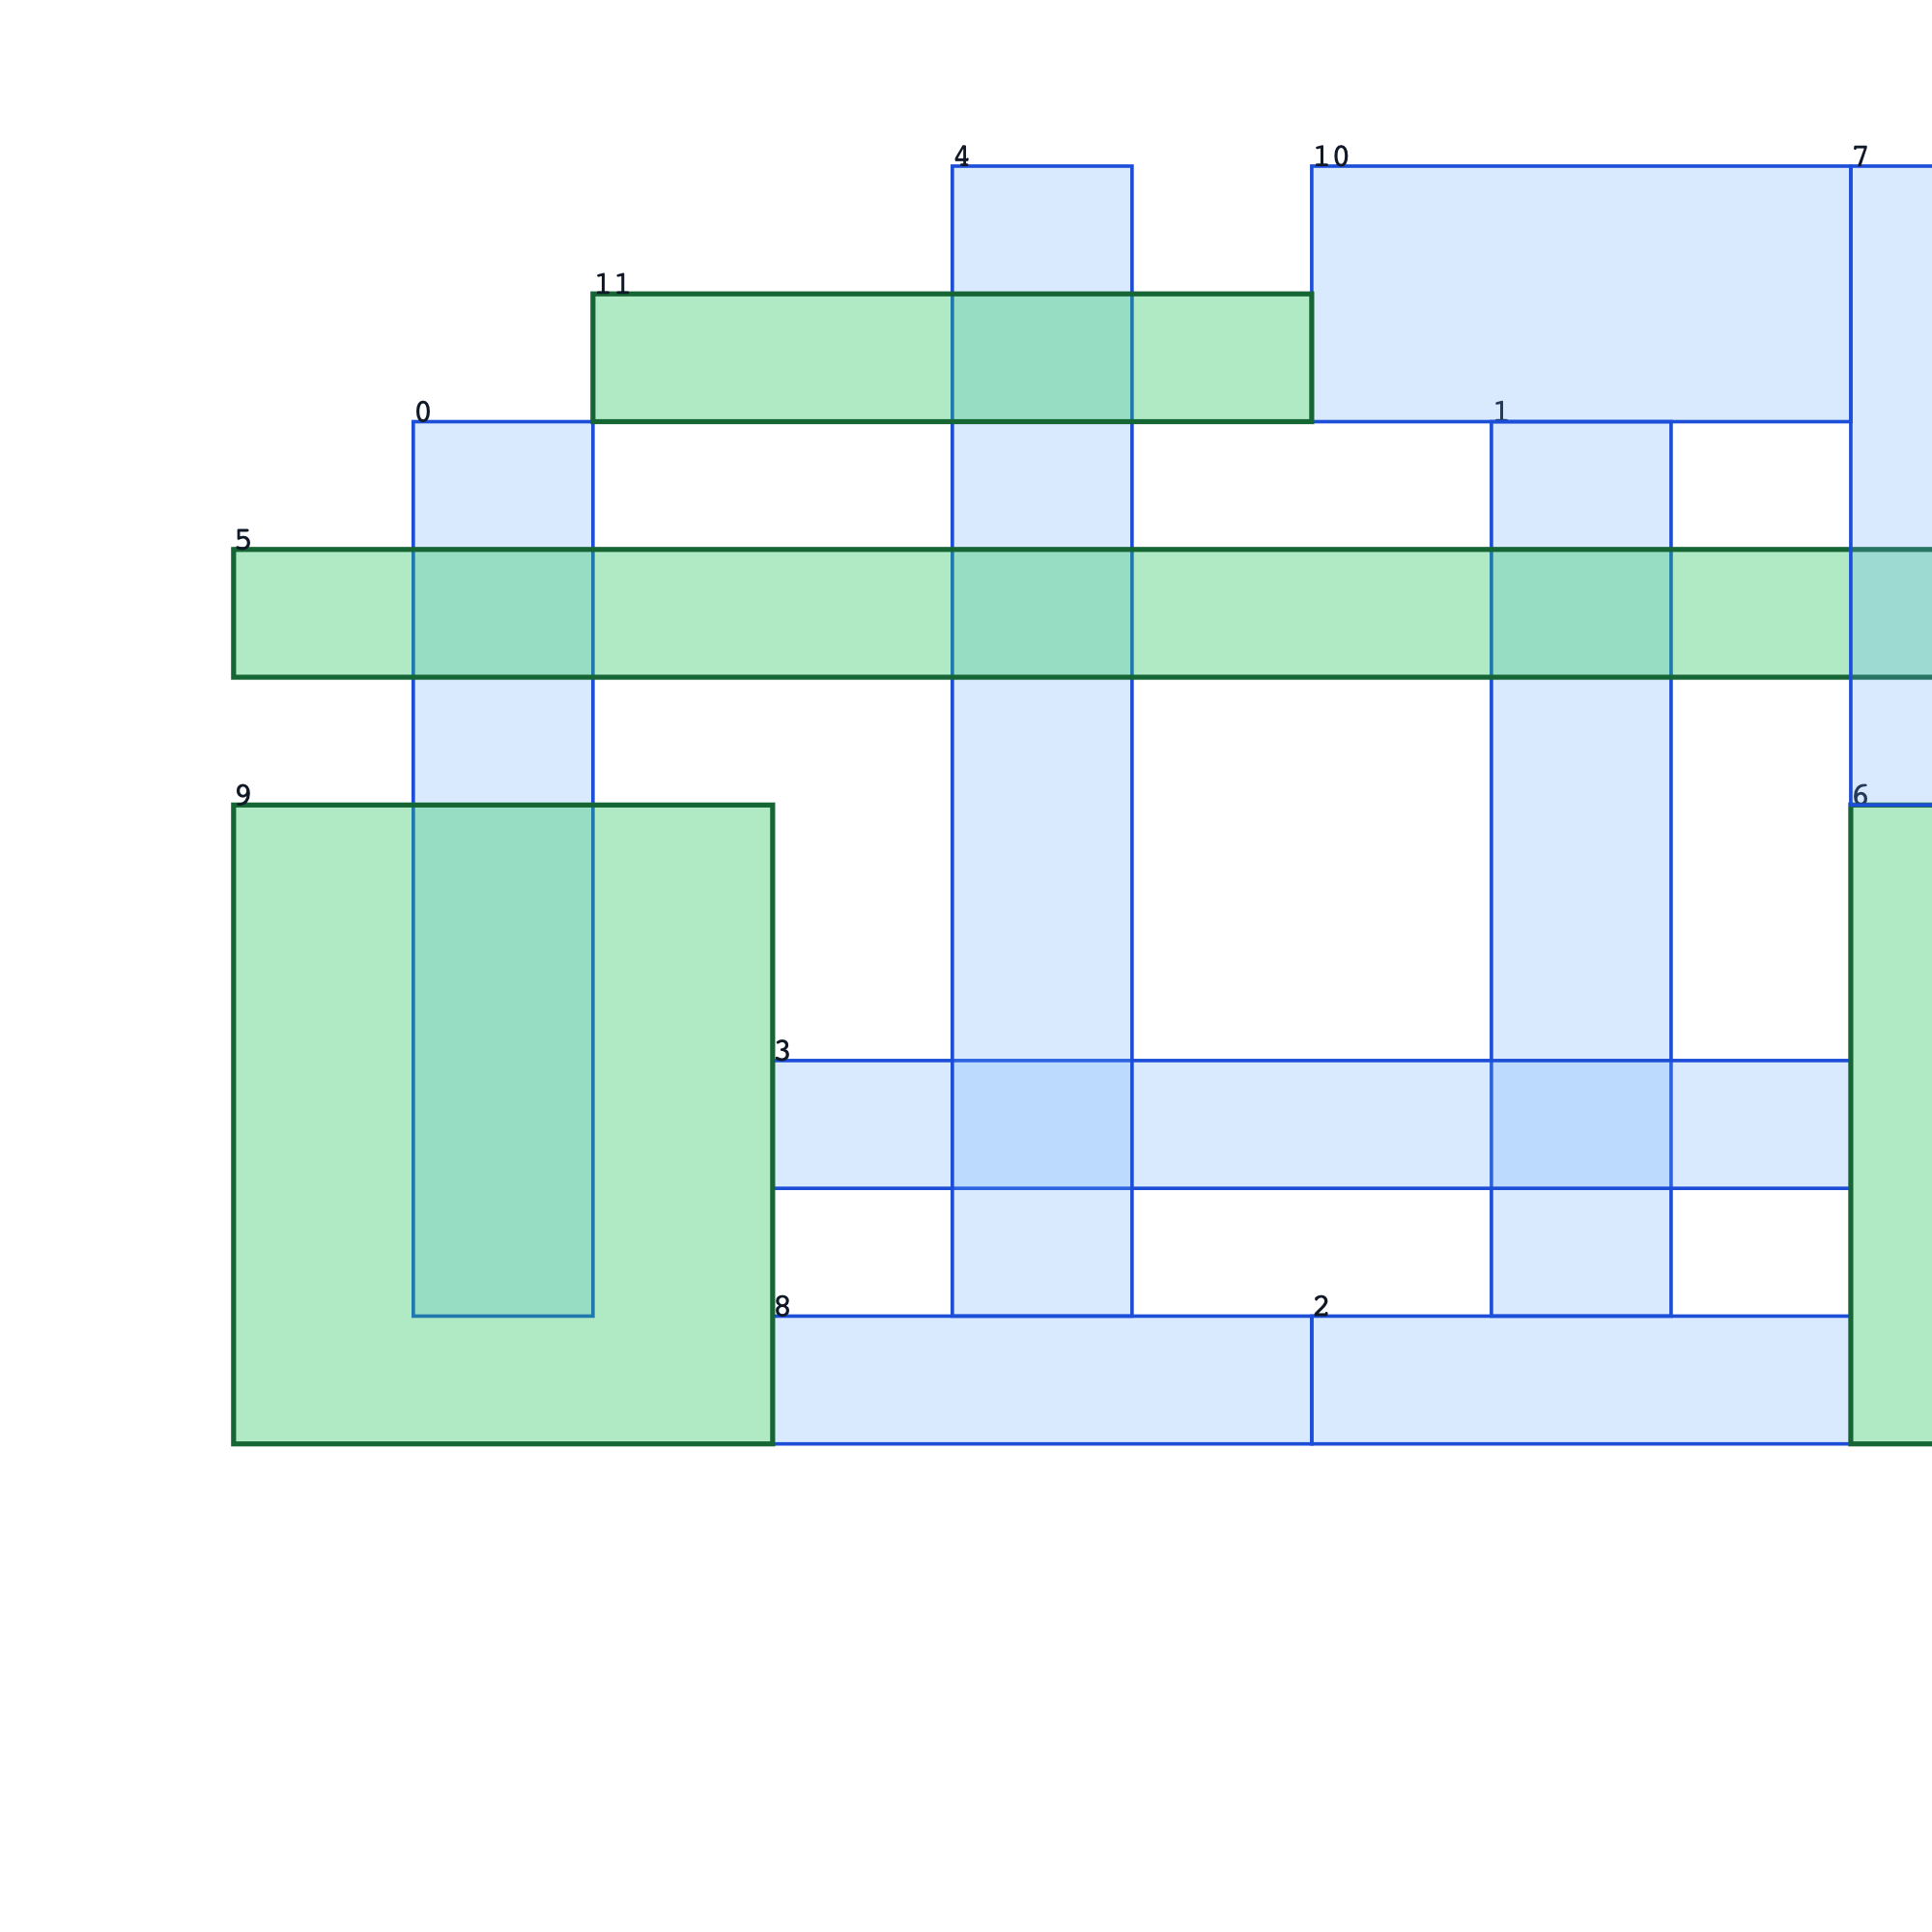
\includegraphics[width=0.82\textwidth]{fig_best_misr.png}
\caption{Best audited MISR construction from the final matrix.  The drawing
is explanatory; the JSON certificate and exact verifier are the evidence.}
\label{fig:misr-best}
\end{figure}

\subsection{Why improvement stopped}

Four mechanisms explain the MISR plateau.

\begin{enumerate}
\item \textbf{Two objectives must move in opposite directions.}  Adding
intersections can raise LP pressure but often also increases the maximum
independent-set structure in a way that leaves the ratio unchanged.
\item \textbf{Triangle-free search has a built-in ceiling mechanism.}  The
clique LP becomes the edge relaxation, and many repaired graphs collapse to
common half-integral ratios.  Repair can delete exactly the vertices that
would have enabled a more unusual denominator.
\item \textbf{The representations lack a reliable composition operator.}
Duplicating a good finite motif usually scales $\alpha$ and $\alpha^*$ at the
same rate, preserving rather than improving the ratio.
\item \textbf{Model training is surrogate-conditioned.}  If the elite archive
contains many geometrically different encodings of the same conflict graph,
the transformer learns syntax and local motif frequency more easily than the
rare global condition that improves $\alpha^*/\alpha$.
\end{enumerate}

The result is a discovery method for compact finite witnesses, not yet an
amplification mechanism for a new asymptotic lower bound.

\clearpage
\section{Problem 2: unit-square line stabbing}

\subsection{Objective and exact verifier}

For a family $\Scal$ of congruent axis-parallel squares,
\[
  \score_{\mathrm{stab}}(\Scal)
  =\frac{\tau(\Scal)}{\tau^*(\Scal)},
\]
where $\tau$ is the minimum number of horizontal and vertical lines stabbing
all squares and $\tau^*$ is the LP optimum over the compressed critical-line
universe.  The certificate stores square coordinates, side length, critical
lines, line-square incidence, an optimal integer cover, LP primal and dual
solutions, and solver status.

\subsection{All 27 trajectories}

\begin{figure}[p]
\centering
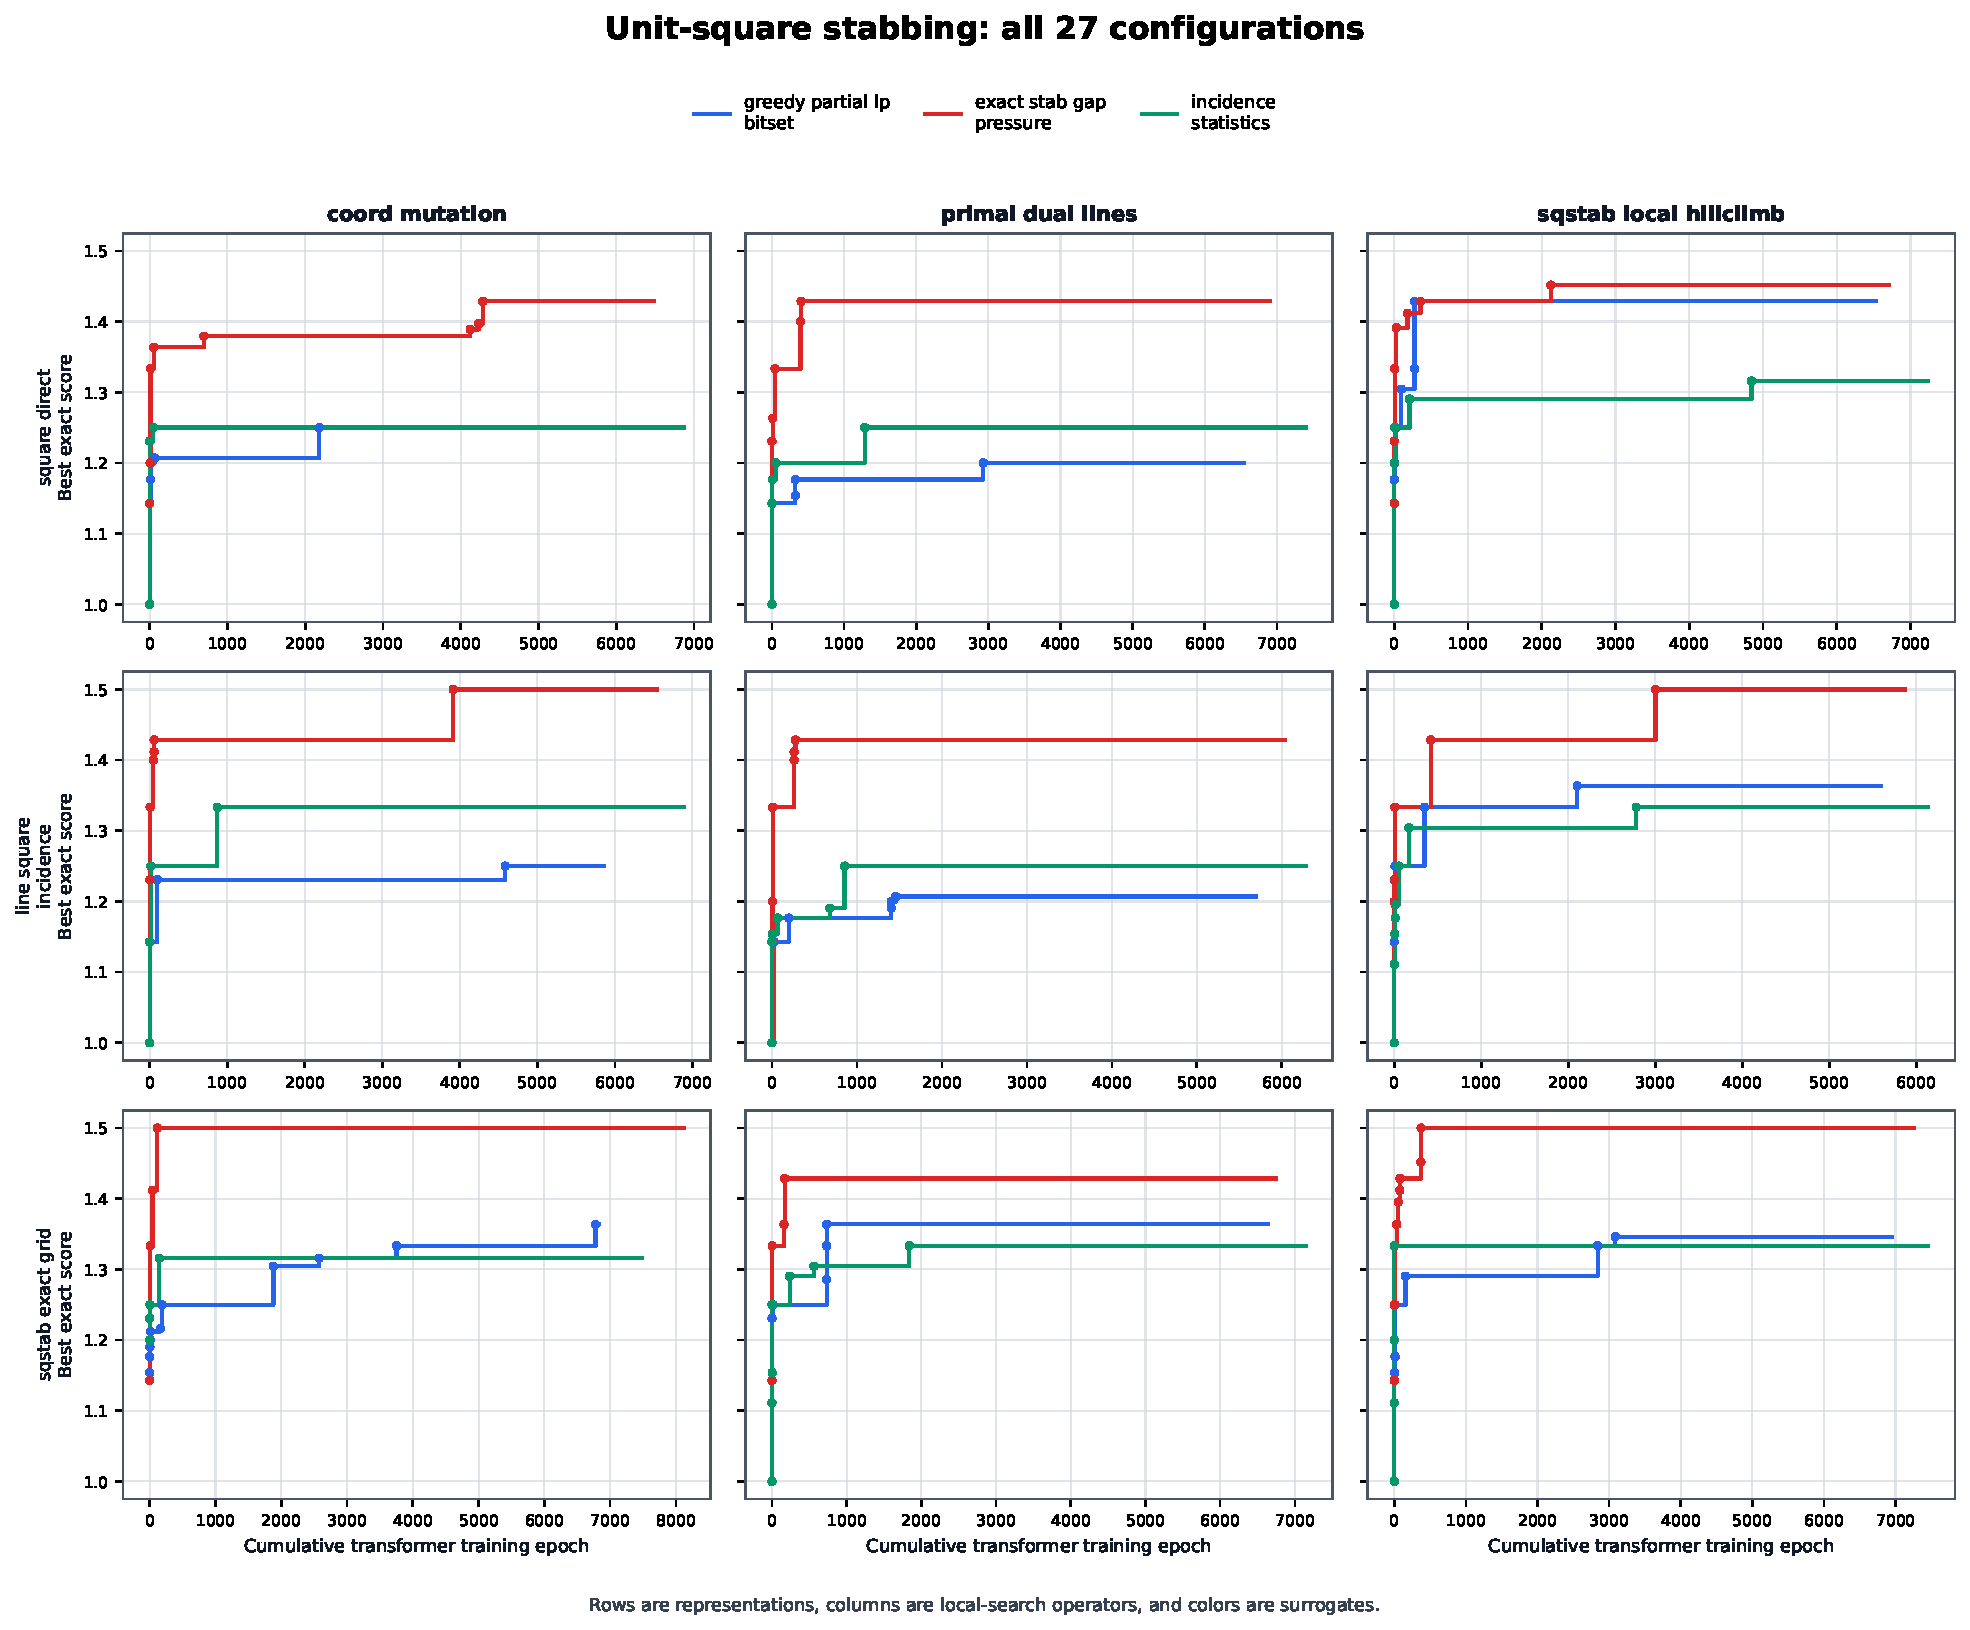
\includegraphics[width=\textwidth]{fig_unit_square_27_trajectories_model_epoch.pdf}
\caption{Unit-square trajectories against cumulative transformer-training
epoch.}
\label{fig:unit-epochs}
\end{figure}

\begin{figure}[p]
\centering
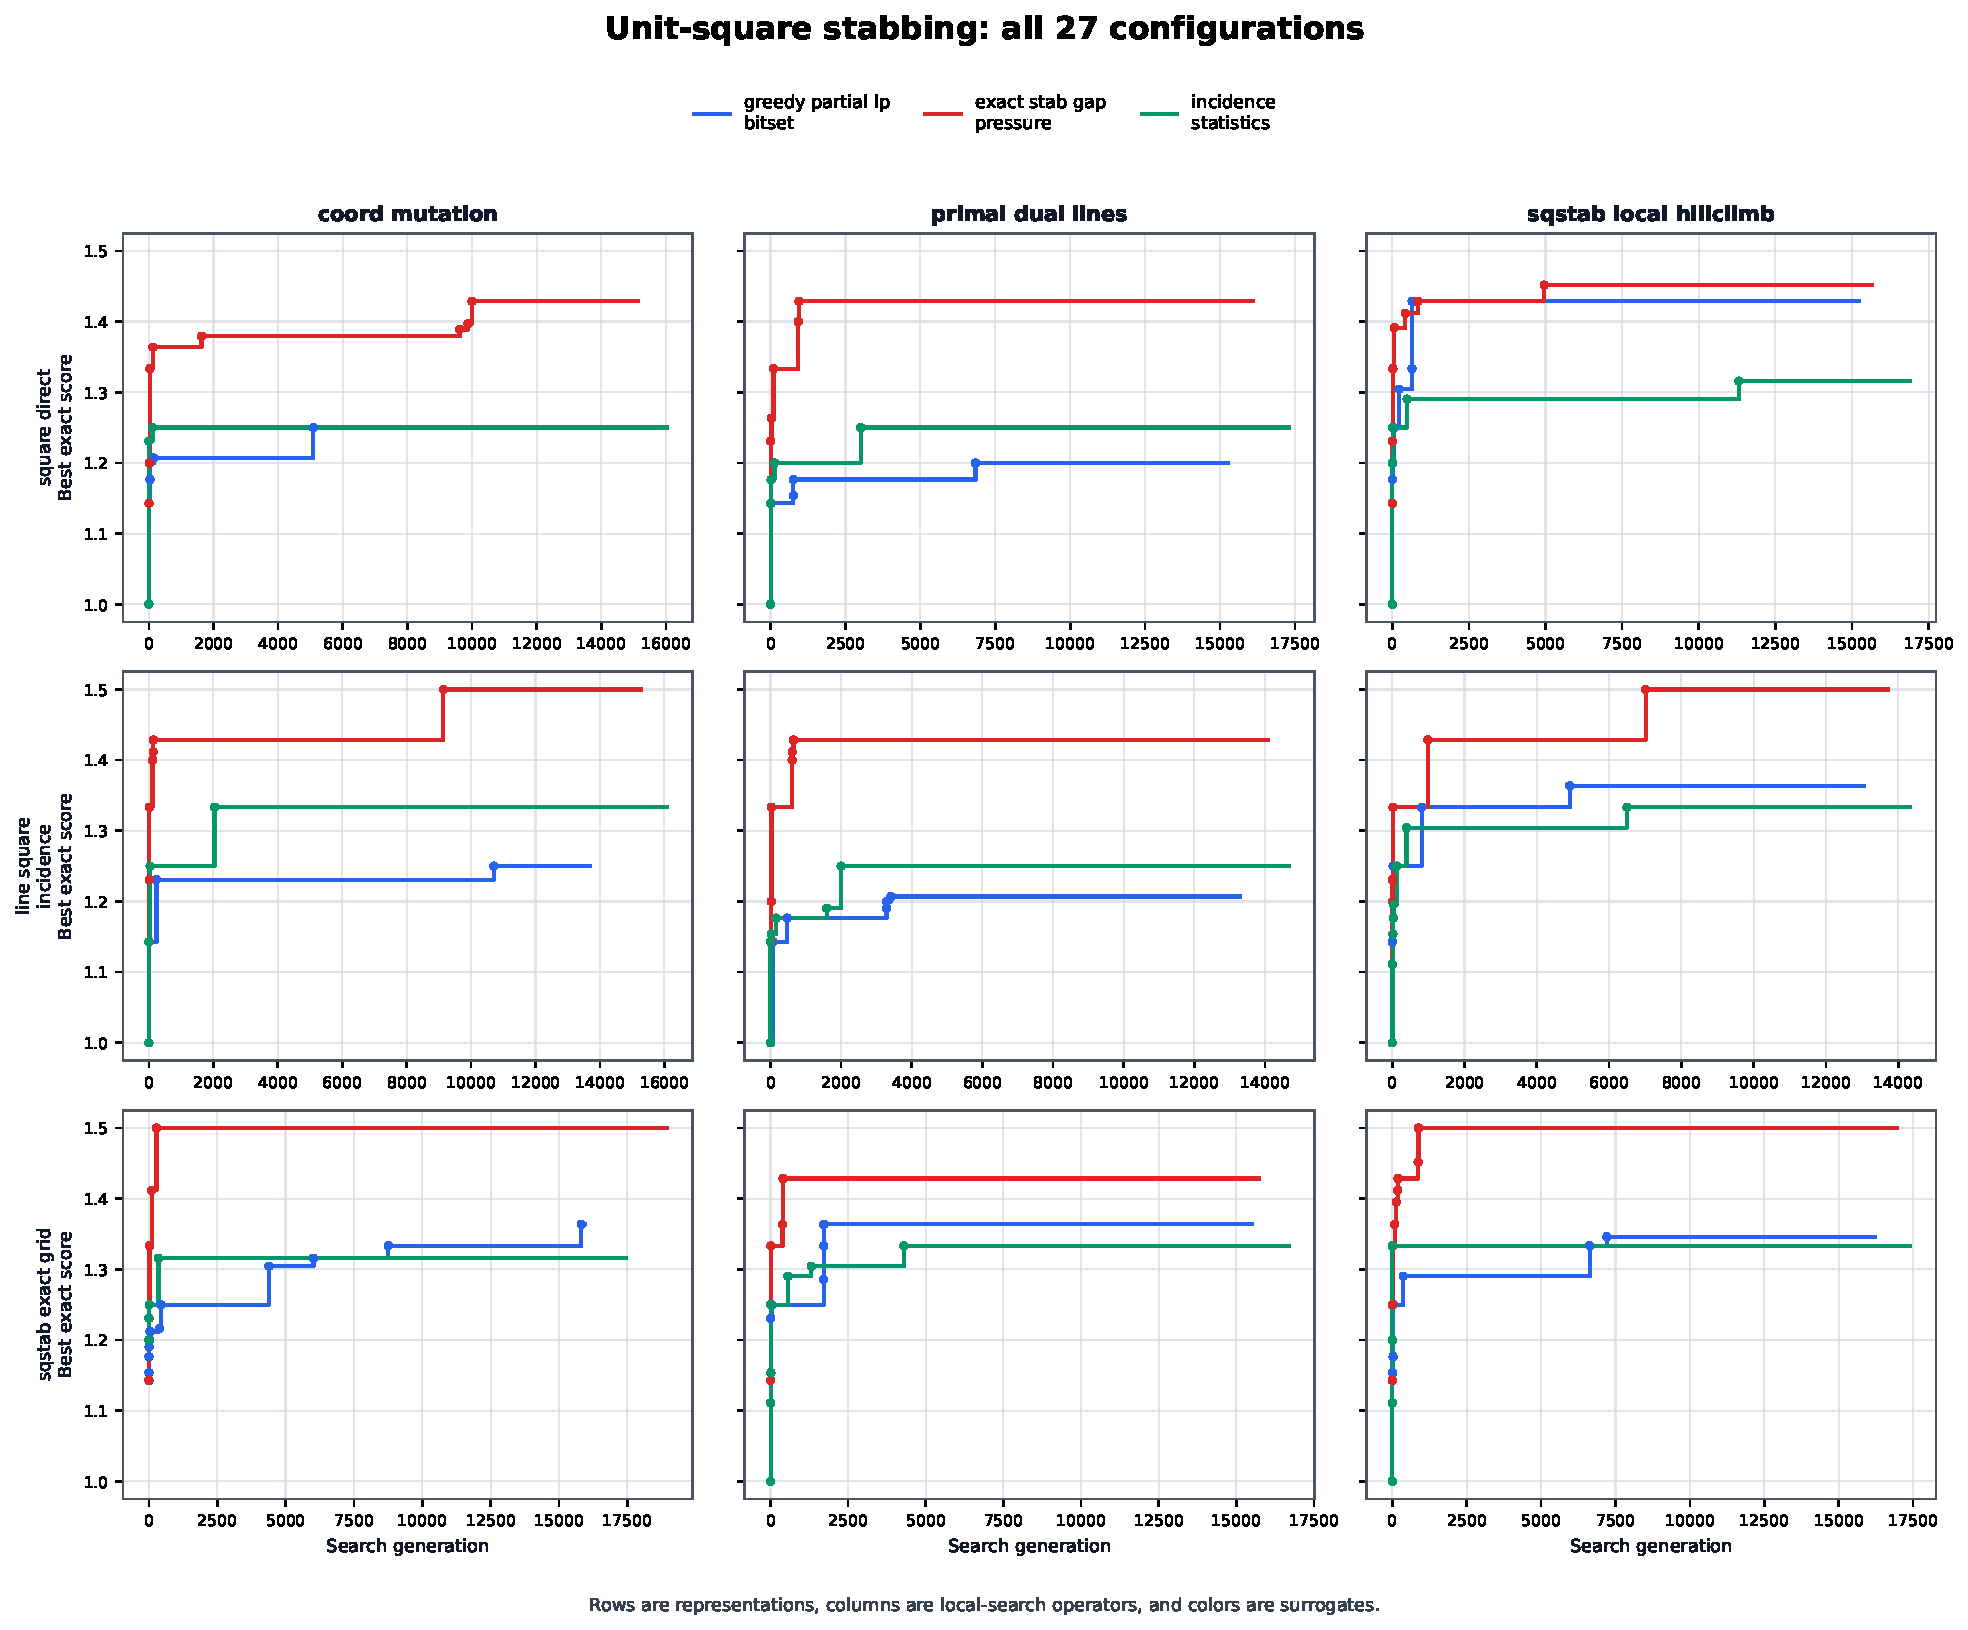
\includegraphics[width=\textwidth]{fig_unit_square_27_trajectories_generation.pdf}
\caption{Unit-square trajectories against search generation.}
\label{fig:unit-generations}
\end{figure}

\begin{table}[tbp]
\centering
\caption{Descriptive component marginals for Unit-square. Each level pools nine distinct component cells.}
\label{tab:unit-square-marginals}
\begin{tabularx}{\textwidth}{p{0.16\textwidth}Xrrrrr}
\toprule
Factor & Level & Mean & Median & Min. & Max. & IQR \\
\midrule
Representation & \code{sqstab\_\allowbreak{}exact\_\allowbreak{}grid} & 1.3872 & 1.3636 & 1.3158 & 1.5000 & [1.3333, 1.4286] \\
 & \code{line\_\allowbreak{}square\_\allowbreak{}incidence} & 1.3518 & 1.3333 & 1.2069 & 1.5000 & [1.2500, 1.4286] \\
 & \code{square\_\allowbreak{}direct} & 1.3337 & 1.3158 & 1.2000 & 1.4516 & [1.2500, 1.4286] \\
\addlinespace
Local Search & \code{sqstab\_\allowbreak{}local\_\allowbreak{}hillclimb} & 1.3969 & 1.3636 & 1.3158 & 1.5000 & [1.3333, 1.4516] \\
 & \code{coord\_\allowbreak{}mutation} & 1.3546 & 1.3333 & 1.2500 & 1.5000 & [1.2500, 1.4286] \\
 & \code{primal\_\allowbreak{}dual\_\allowbreak{}lines} & 1.3211 & 1.3333 & 1.2000 & 1.4286 & [1.2500, 1.4286] \\
\addlinespace
Surrogate & \code{exact\_\allowbreak{}stab\_\allowbreak{}gap\_\allowbreak{}pressure} & 1.4629 & 1.4516 & 1.4286 & 1.5000 & [1.4286, 1.5000] \\
 & \code{greedy\_\allowbreak{}partial\_\allowbreak{}lp\_\allowbreak{}bitset} & 1.3081 & 1.3462 & 1.2000 & 1.4286 & [1.2500, 1.3636] \\
 & \code{incidence\_\allowbreak{}statistics} & 1.3017 & 1.3158 & 1.2500 & 1.3333 & [1.2500, 1.3333] \\
\addlinespace
\bottomrule
\end{tabularx}
\end{table}


Unit-square stabbing has the strongest single component effect in the entire
study.  The exact gap surrogate averages $1.4629$ and every one of its nine
cells lies between $10/7$ and $3/2$.  The greedy and incidence-statistics
surrogates average only $1.3081$ and $1.3017$.  Thus additional generations
under a cheap proxy do not compensate for optimizing the wrong quantity.  The
\code{sqstab\_exact\_grid} representation has the strongest representation
mean ($1.3872$), while \code{sqstab\_local\_hillclimb} has the strongest local
search mean ($1.3969$).  Four exact-pressure cells reach numerical $3/2$,
showing that this plateau is reproducible across multiple component paths even
without repeated seeds.

\subsection{What worked}

The successful paths optimize the geometric set-cover instance through its
critical-line incidence rather than treating coordinates as independent
numbers.  Exact gap pressure is particularly valuable because greedy cover
size, maximum line frequency, and incidence balance are not reliable proxies
for the LP optimum.  Coordinate mutation can still help when it crosses a
critical endpoint and therefore changes several incidence relations at once.

\begin{figure}[tbp]
\centering
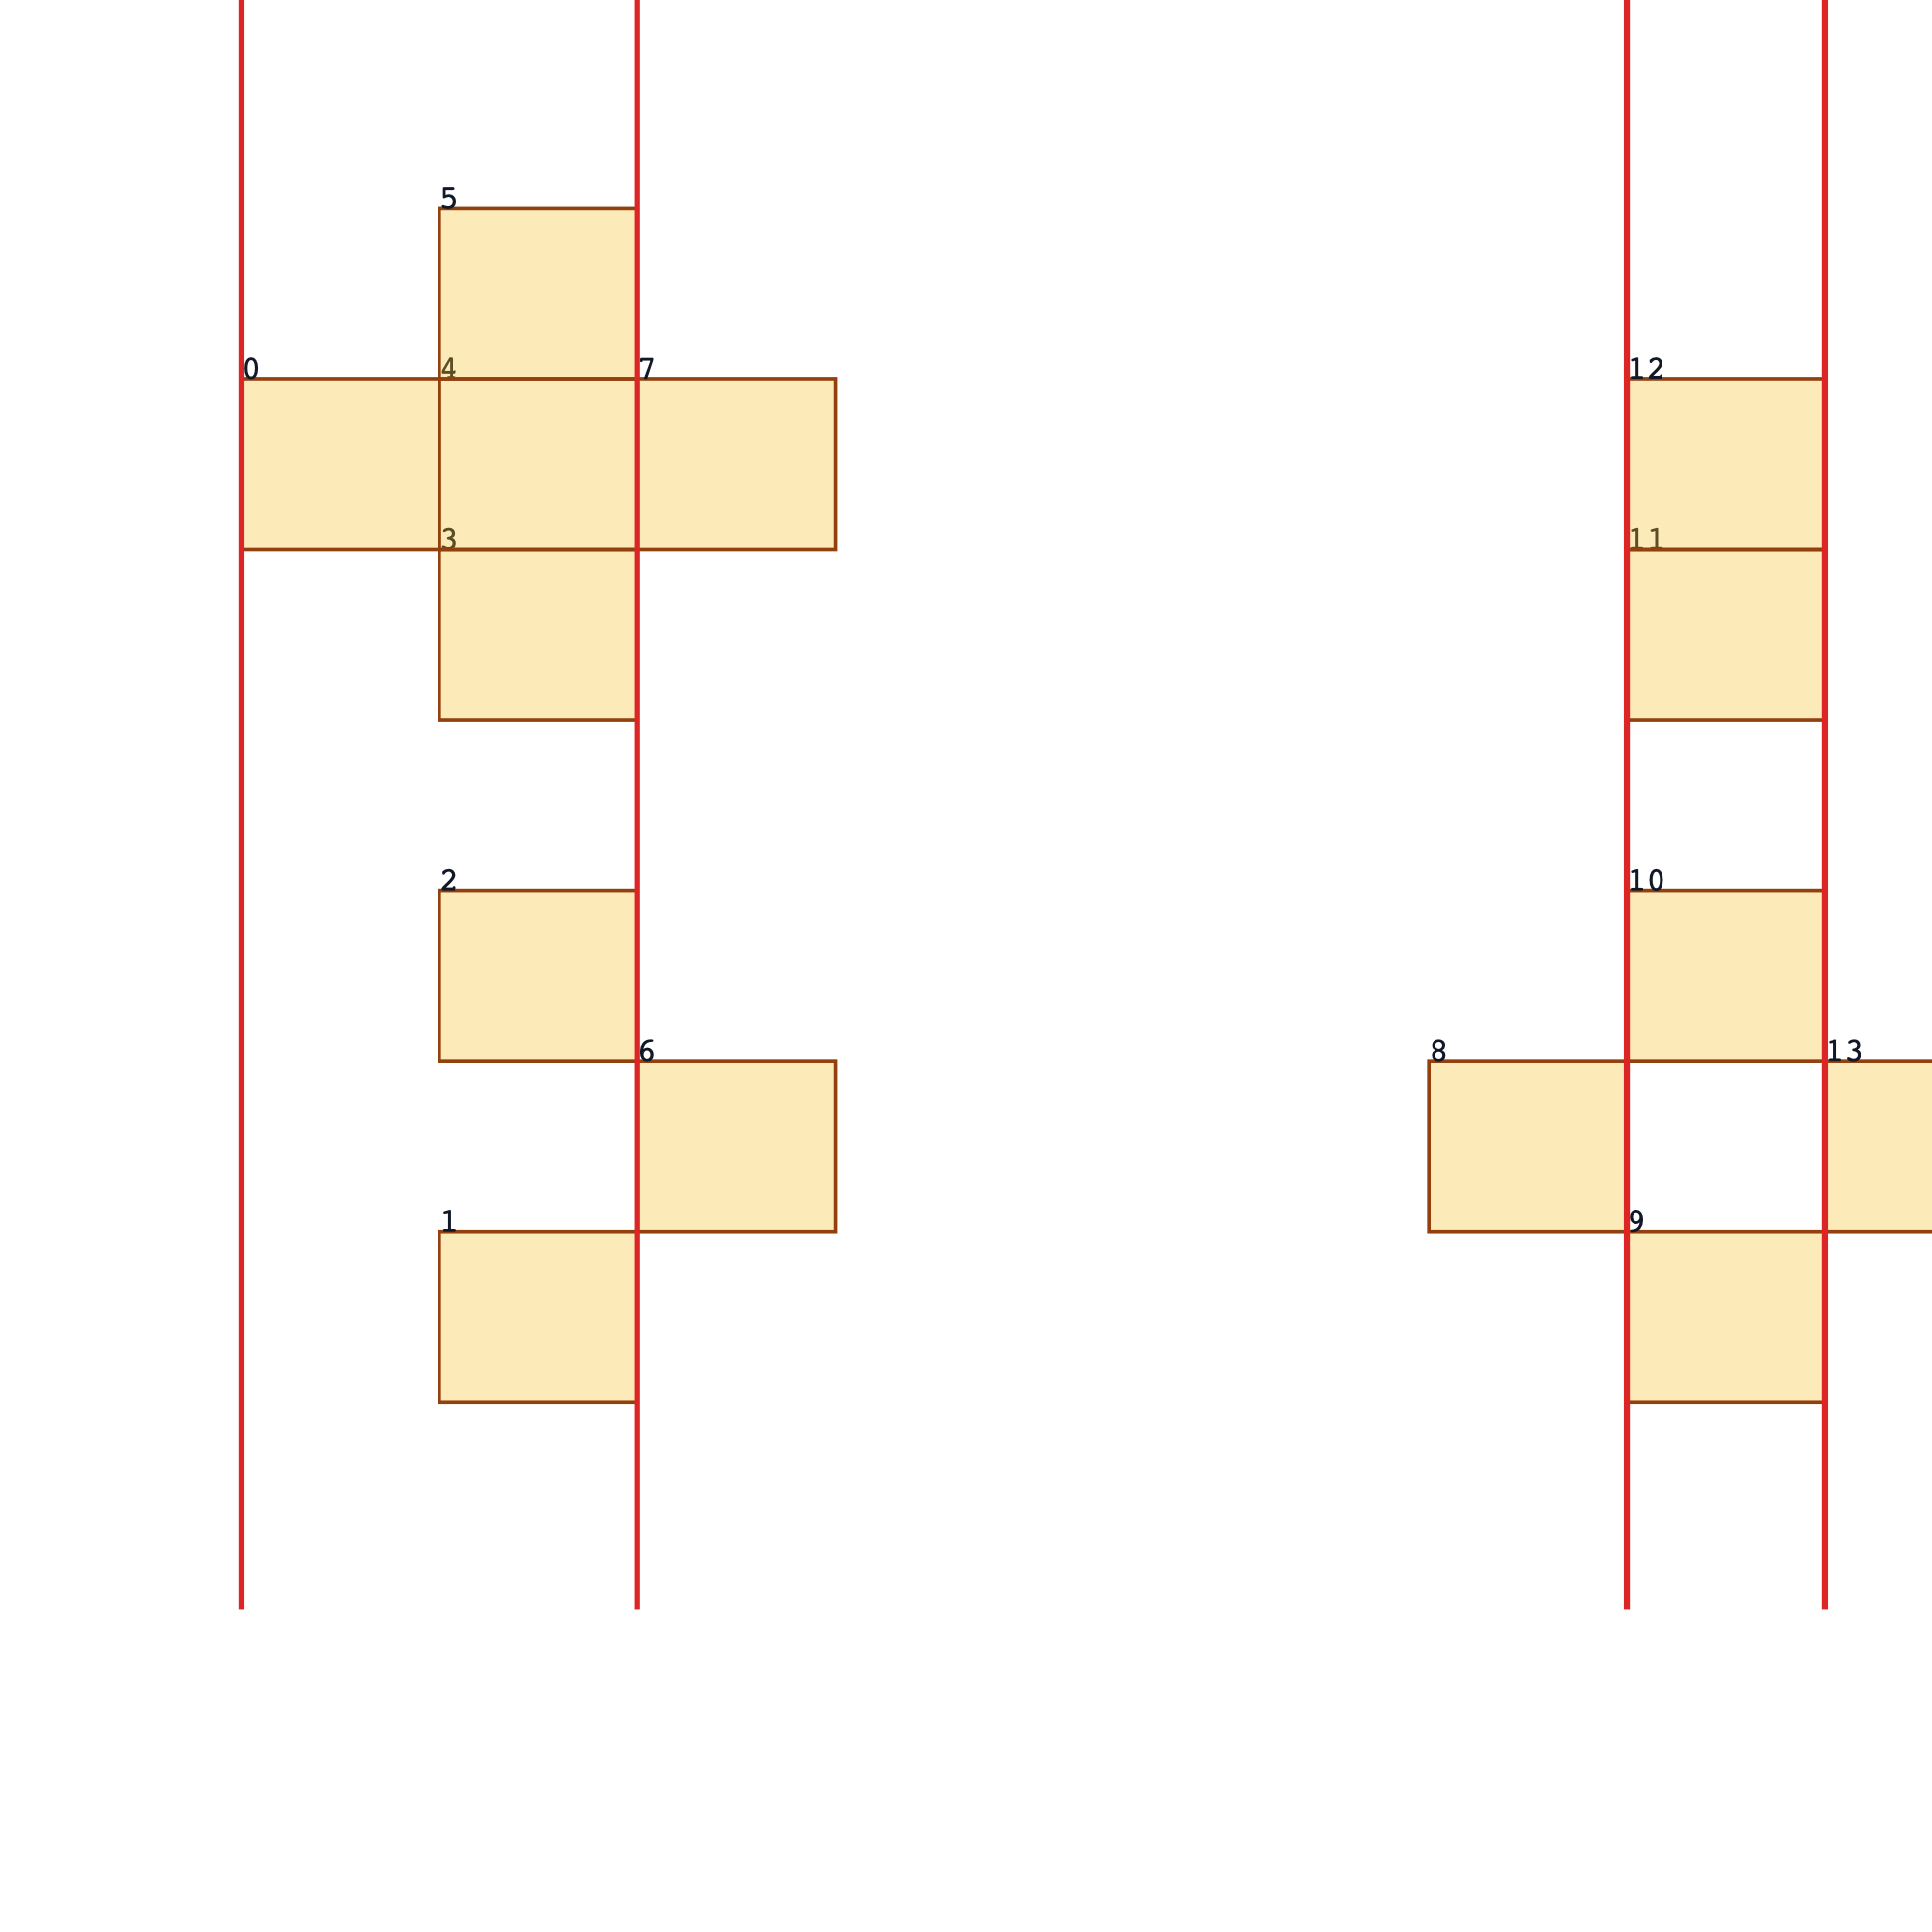
\includegraphics[width=0.76\textwidth]{fig_best_unit_square.png}
\caption{Best audited unit-square stabbing construction from the final
matrix.}
\label{fig:unit-best}
\end{figure}

\subsection{Why improvement stopped}

The unit-square plateau is strongly discrete.  A local move usually preserves
the same critical-line incidence matrix and therefore leaves both $\tau$ and
$\tau^*$ unchanged.  A threshold-crossing move often changes the integer and
fractional optima together.  The search operates on an integer coordinate
grid with 8--24 accepted squares, so it explores only a small part of the
realizable incidence landscape.  Moreover, the generic model learns a
serialization of coordinates; it has no explicit equivariance under
translation, relabeling, or affine normalization.

The observed $3/2$-type behavior is compact and repeatedly rediscovered, but
the code has no neutral, general composition rule that combines such blocks
without allowing one line to stab multiple blocks.  That cross-block line is
the geometric reason direct sums fail to amplify the set-cover gap.

\clearpage
\section{Problem 3: recursive guillotine hardness}

\subsection{Objective and exact verifier}

For a pairwise interior-disjoint rectangle family $\Rcal$,
\[
  \score_{\mathrm{guill}}(\Rcal)
  =1-\frac{\save(\Rcal)}{|\Rcal|},
\]
where $\save(\Rcal)$ is the maximum number of rectangles preserved by an
optimal recursive sequence of horizontal and vertical guillotine cuts.  The
exact dynamic program enumerates coordinate-induced cuts on rectangle-subset
states.  Its certificate stores the exact saved and destroyed counts, the
optimal recursive cut tree, first-cut diagnostics, threshold diagnostics,
state count, and solver status.

\subsection{All 27 trajectories}

\begin{figure}[p]
\centering
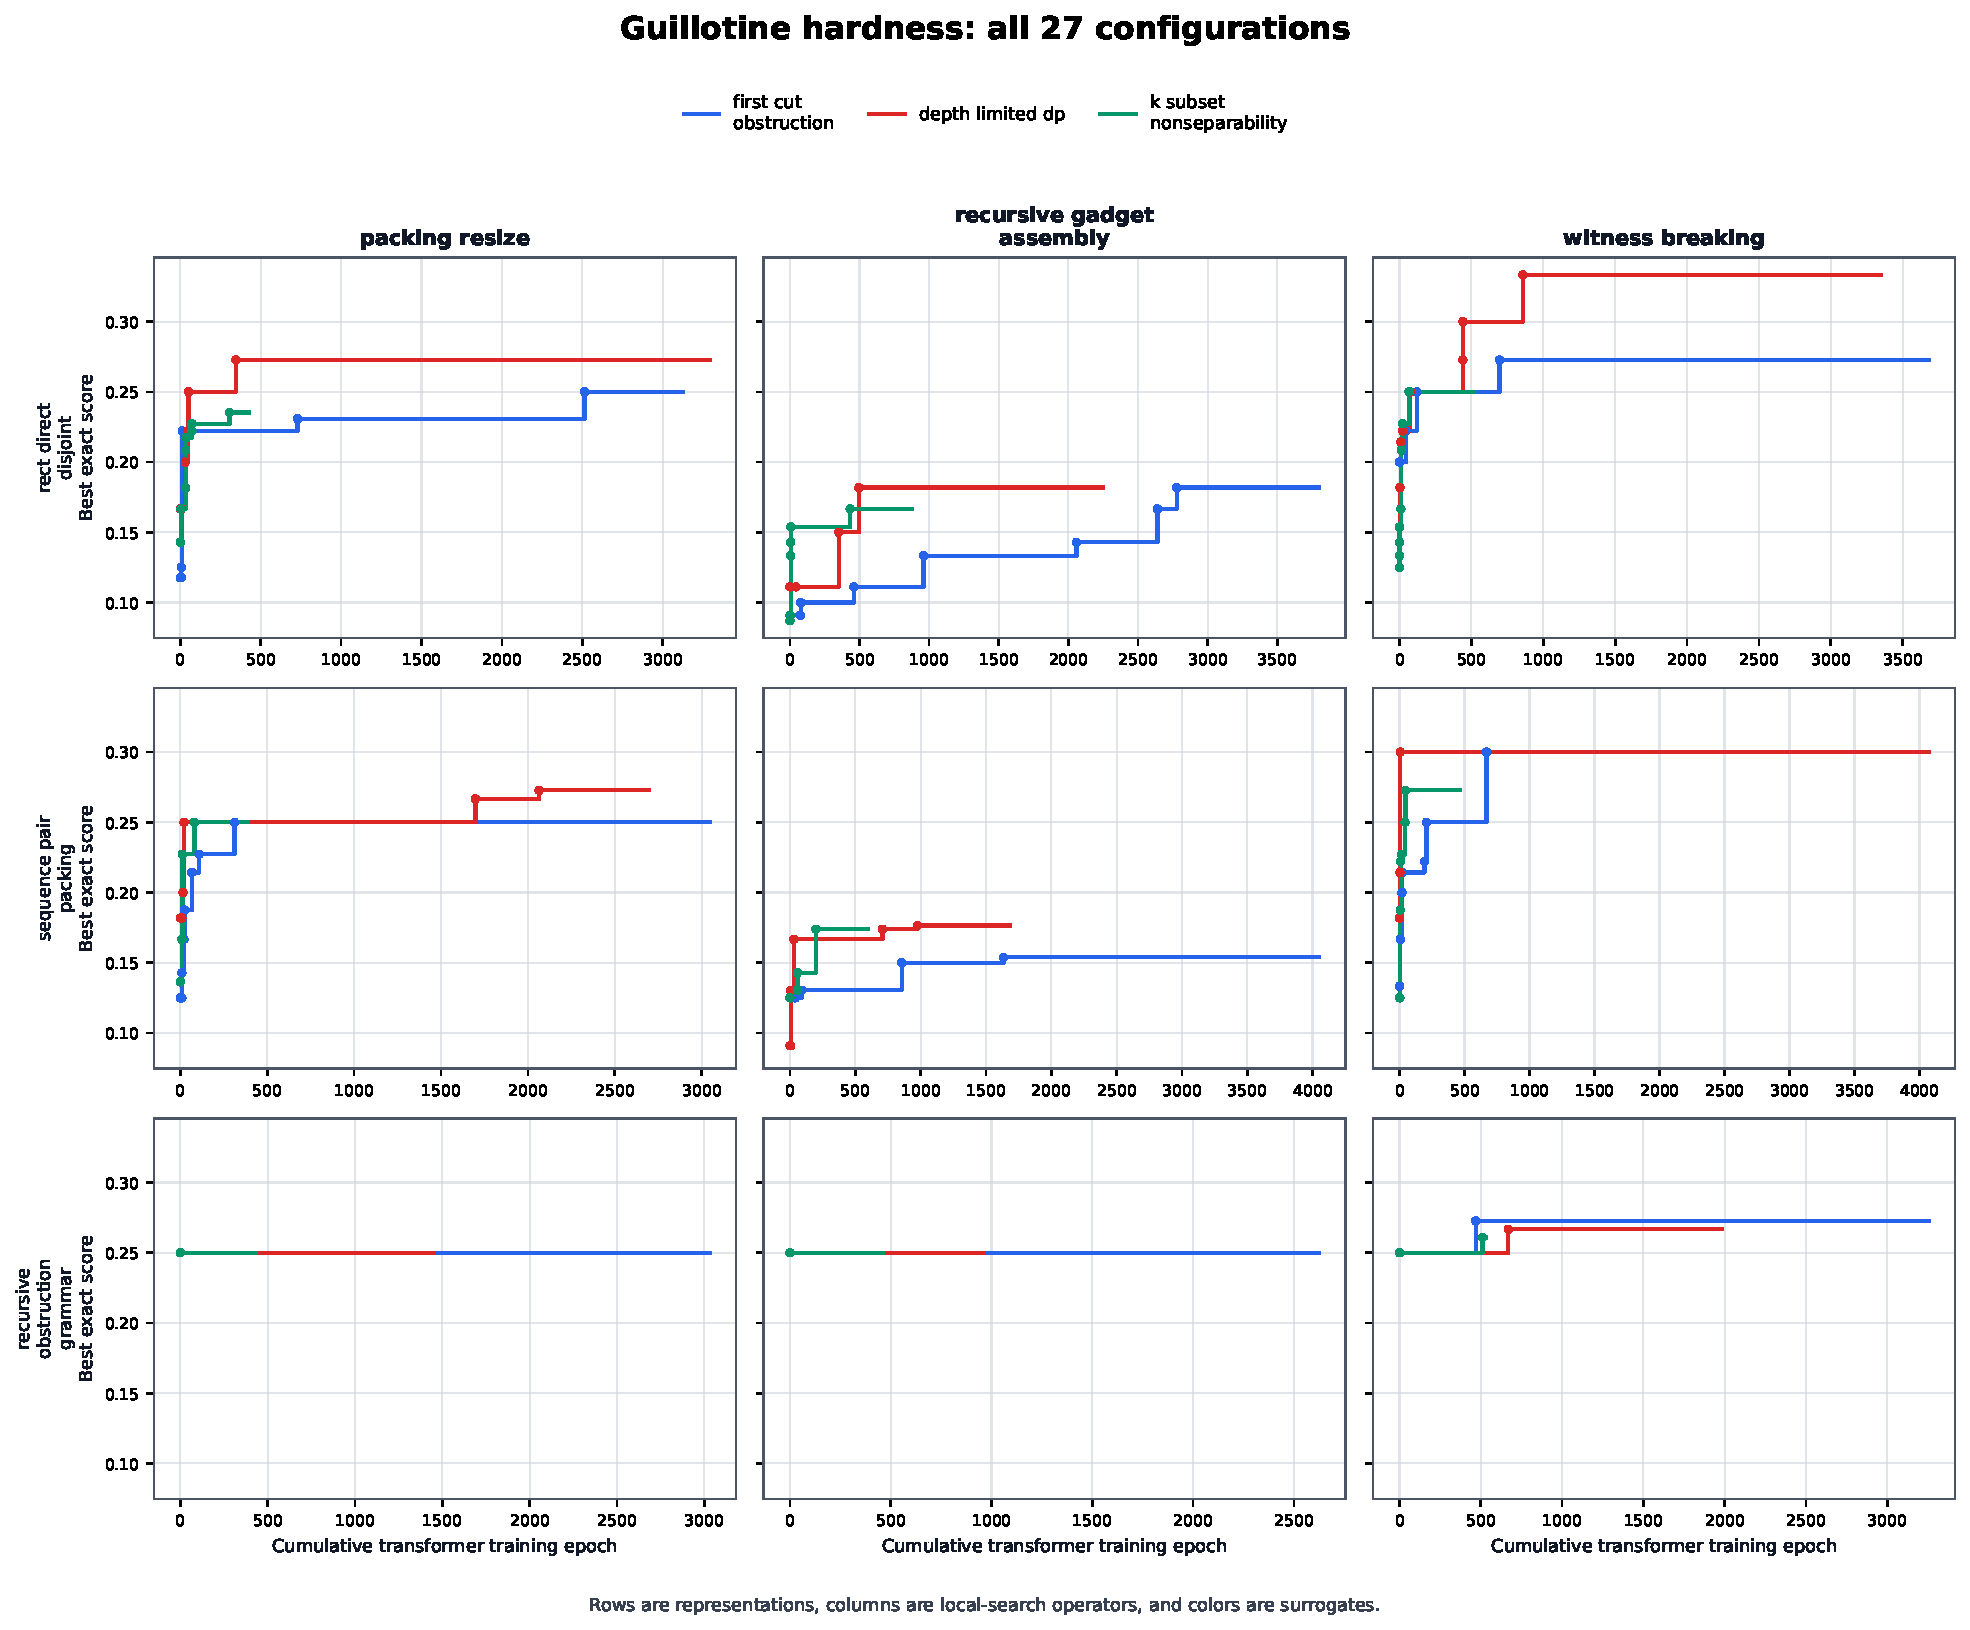
\includegraphics[width=\textwidth]{fig_guillotine_27_trajectories_model_epoch.pdf}
\caption{Guillotine trajectories against cumulative transformer-training
epoch.}
\label{fig:guillotine-epochs}
\end{figure}

\begin{figure}[p]
\centering
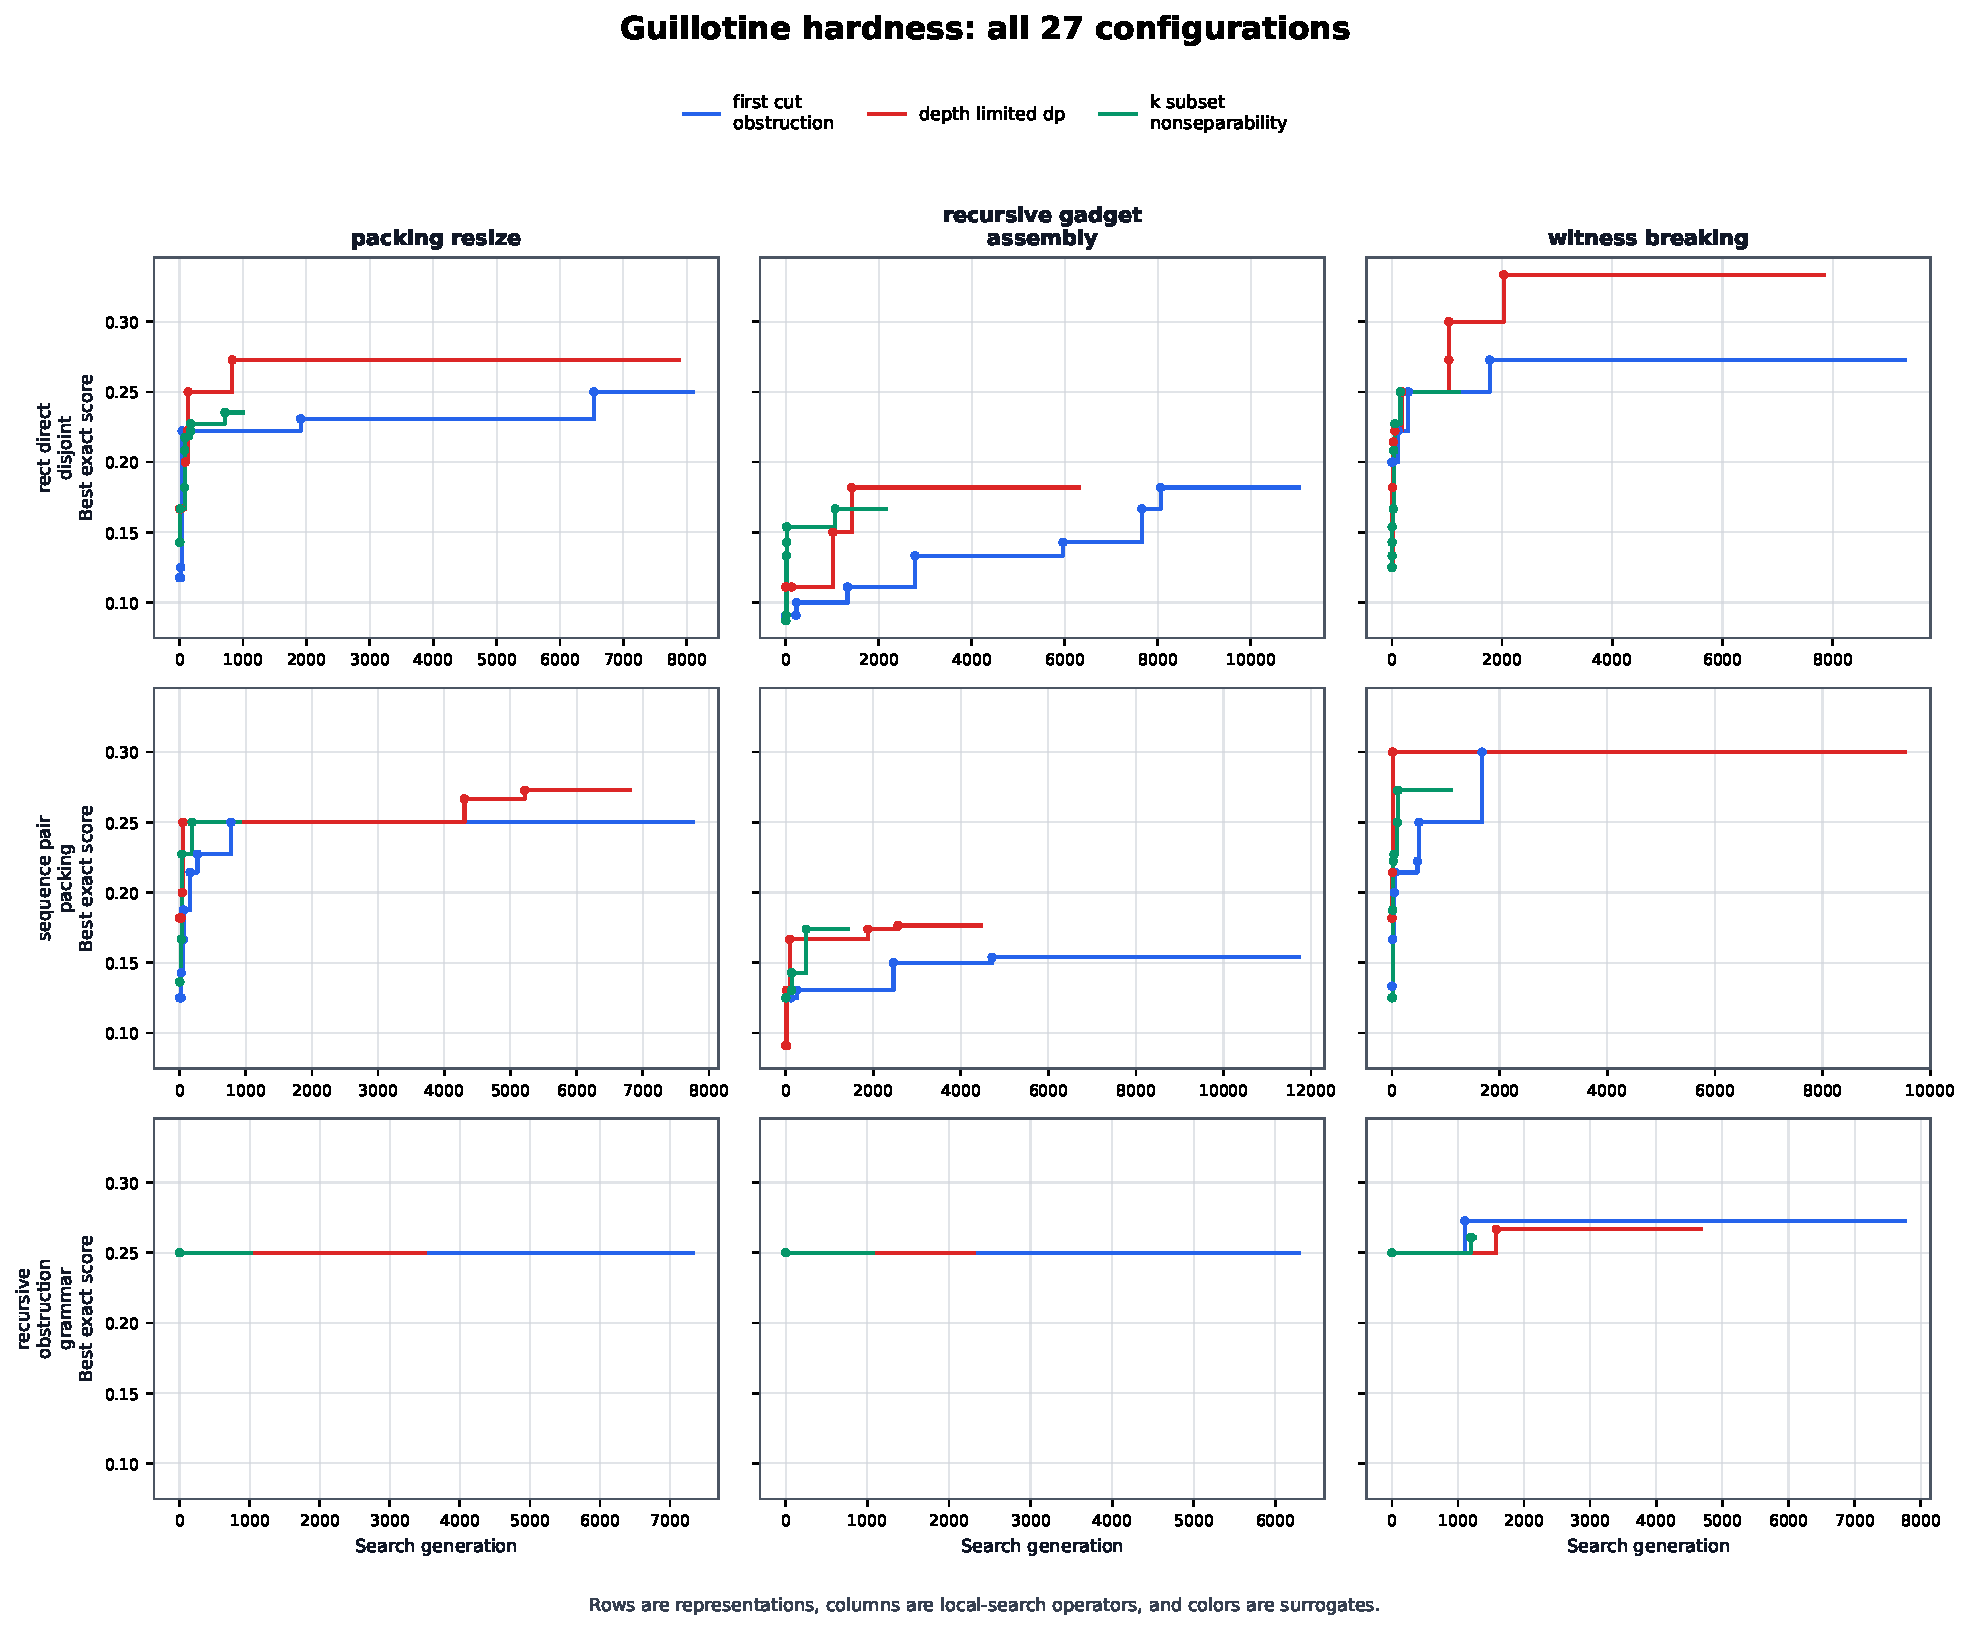
\includegraphics[width=\textwidth]{fig_guillotine_27_trajectories_generation.pdf}
\caption{Guillotine trajectories against search generation.}
\label{fig:guillotine-generations}
\end{figure}

\begin{table}[tbp]
\centering
\caption{Descriptive component marginals for Guillotine. Each level pools nine distinct component cells.}
\label{tab:guillotine-marginals}
\begin{tabularx}{\textwidth}{p{0.16\textwidth}Xrrrrr}
\toprule
Factor & Level & Mean & Median & Min. & Max. & IQR \\
\midrule
Representation & \code{recursive\_\allowbreak{}obstruction\_\allowbreak{}grammar} & 0.2556 & 0.2500 & 0.2500 & 0.2727 & [0.2500, 0.2609] \\
 & \code{sequence\_\allowbreak{}pair\_\allowbreak{}packing} & 0.2389 & 0.2500 & 0.1538 & 0.3000 & [0.1765, 0.2727] \\
 & \code{rect\_\allowbreak{}direct\_\allowbreak{}disjoint} & 0.2383 & 0.2500 & 0.1667 & 0.3333 & [0.1818, 0.2727] \\
\addlinespace
Local Search & \code{witness\_\allowbreak{}breaking} & 0.2810 & 0.2727 & 0.2500 & 0.3333 & [0.2667, 0.3000] \\
 & \code{packing\_\allowbreak{}resize} & 0.2534 & 0.2500 & 0.2353 & 0.2727 & [0.2500, 0.2500] \\
 & \code{recursive\_\allowbreak{}gadget\_\allowbreak{}assembly} & 0.1983 & 0.1818 & 0.1538 & 0.2500 & [0.1739, 0.2500] \\
\addlinespace
Surrogate & \code{depth\_\allowbreak{}limited\_\allowbreak{}dp} & 0.2560 & 0.2667 & 0.1765 & 0.3333 & [0.2500, 0.2727] \\
 & \code{first\_\allowbreak{}cut\_\allowbreak{}obstruction} & 0.2423 & 0.2500 & 0.1538 & 0.3000 & [0.2500, 0.2727] \\
 & \code{k\_\allowbreak{}subset\_\allowbreak{}nonseparability} & 0.2344 & 0.2500 & 0.1667 & 0.2727 & [0.2353, 0.2500] \\
\addlinespace
\bottomrule
\end{tabularx}
\end{table}


The guillotine matrix shows that witness use matters more than a more elaborate
generator label.  \code{witness\_breaking} averages $0.2810$, compared with
$0.2534$ for \code{packing\_resize} and only $0.1983$ for
\code{recursive\_gadget\_assembly}.  The latter often adds or copies local
blocks without closing the recursive escape route and is actively harmful in
this matrix.  Among surrogates, \code{depth\_limited\_dp} is strongest on
average ($0.2560$), while \code{k\_subset\_nonseparability} is weakest
($0.2344$) despite being more elaborate.  The recursive-obstruction
representation is stable but capped between $0.25$ and $0.2727$; direct
disjoint search is more variable and contains both weaker rows and the unique
$1/3$ record.  This is a useful distinction between robust initialization and
record potential.

\subsection{What worked}

Guillotine search improves when the representation supplies non-sliceable
local structure and the mutation operator responds to actual separable
subsets.  Witness breaking and packing resize can close easy projection gaps;
the depth-limited dynamic program is more aligned with the exact recursive
objective than first-cut obstruction.  The $k$-subset surrogate adds useful
large-subset pressure, although it is sampled above 16 rectangles.

\begin{figure}[tbp]
\centering
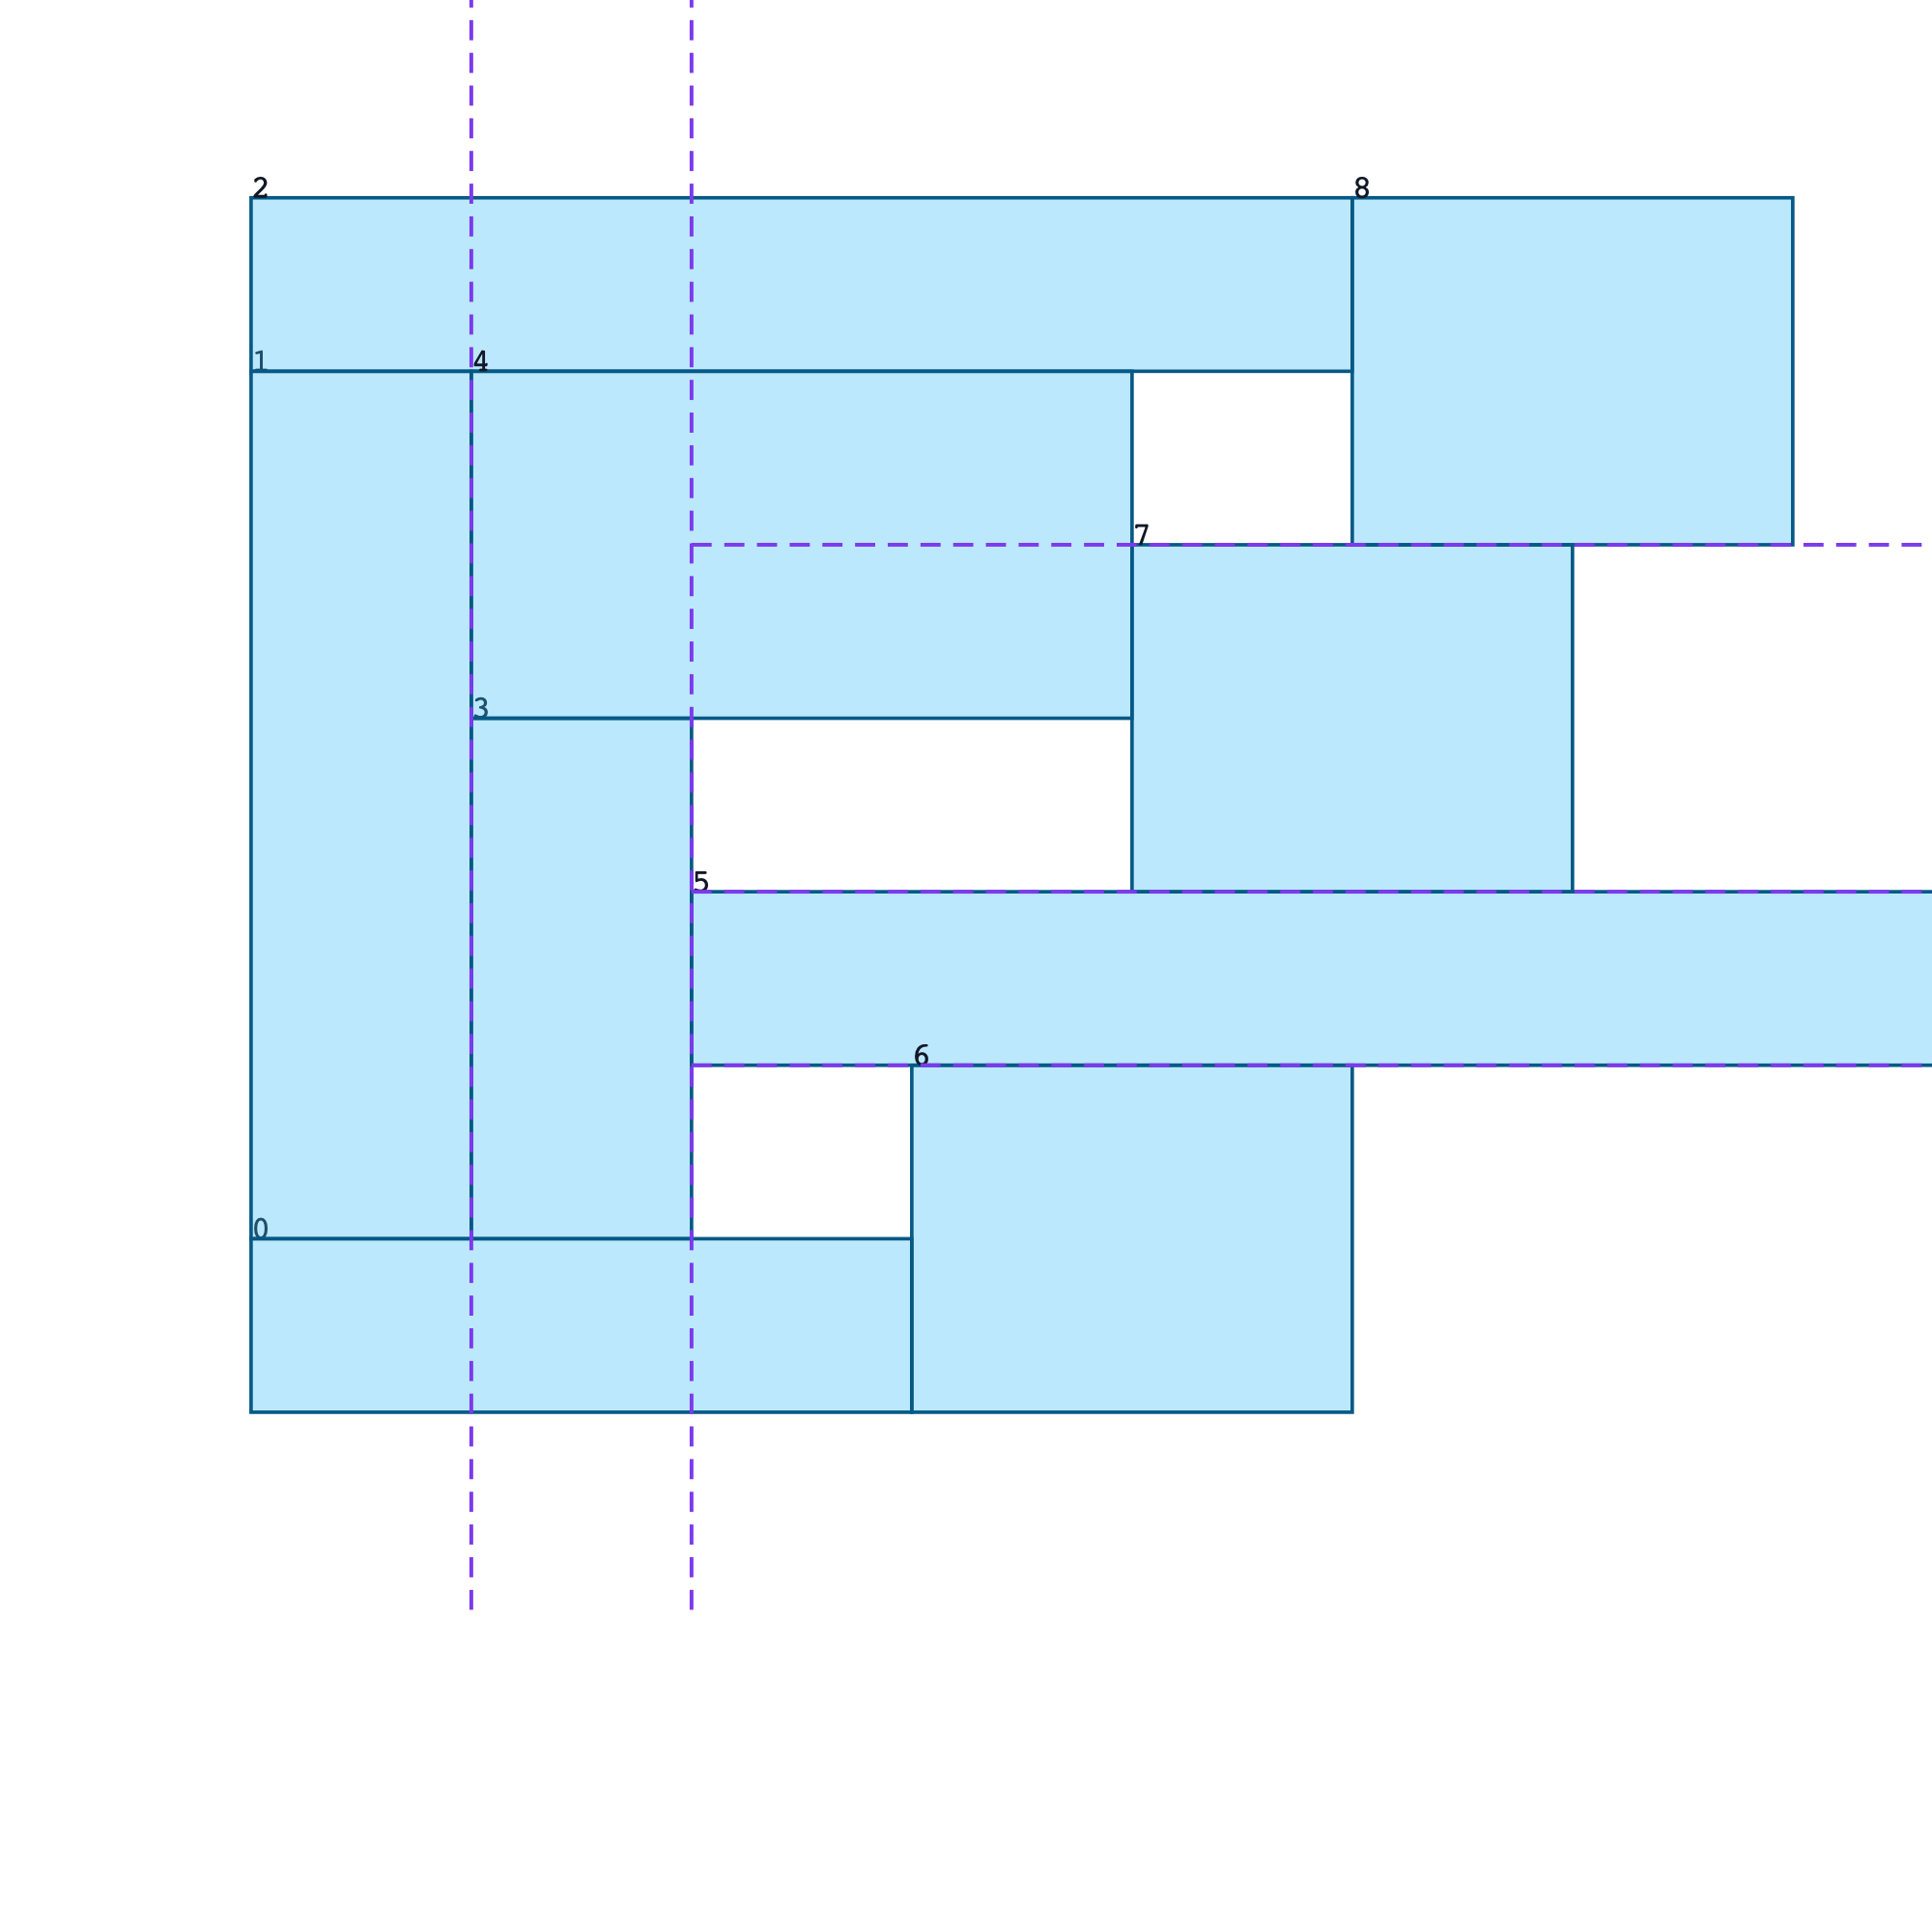
\includegraphics[width=0.82\textwidth]{fig_best_guillotine.png}
\caption{Best audited guillotine construction from the final matrix.  The
exact cut tree in the certificate, not the drawing, establishes the saved and
destroyed counts.}
\label{fig:guillotine-best}
\end{figure}

\subsection{Why improvement stopped}

Guillotine hardness is the clearest case of surrogate mismatch.

\begin{enumerate}
\item \textbf{First-cut obstruction is not recursive obstruction.}  A layout
can force an expensive first cut while leaving two easy subinstances.
\item \textbf{Depth four is still shallow.}  The depth-limited surrogate
returns all remaining rectangles as saveable at its horizon, favoring layouts
whose weakness appears just beyond that depth.
\item \textbf{Large-$n$ threshold tests are sampled.}  The deterministic
subset schedule is reproducible, but 1024 subsets cannot represent all
$\binom{n}{\lfloor n/2\rfloor+1}$ possibilities.  High sampled
nonseparability can coexist with a large exact saved set.
\item \textbf{The score has coarse rational steps.}  With $n$ rectangles the
score changes in increments of $1/n$.  Mutations that add easy filler
rectangles can make the layout look larger while reducing the destroyed
fraction.
\item \textbf{Exact feedback arrives only on elites.}  The exact cut tree is
saved in a certificate but is not fully converted into a differentiable or
dense training signal for every candidate.
\end{enumerate}

The fixed spiral topology used by one representation is also a methodological
limitation: it can improve the chance of seeing a local obstruction, but it
narrows the search toward one family.  The representation comparison must
therefore be read as ``which supplied search family worked best,'' not as a
neutral estimate over all disjoint rectangle packings.

\clearpage
\section{Cross-problem explanation of the barriers}

\subsection{Prioritized diagnosis}

Table~\ref{tab:limitations} ranks the limitations by their likely leverage on
future search.  The ranking is a mechanistic interpretation of the completed
matrix, not a causal effect estimate: there is one stochastic run per cell.

\begin{table}[p]
\centering
\small
\caption{Prioritized limitations supported by the 81-run evidence.  ``Likely
leverage'' estimates how strongly fixing the limitation could change the
reachable constructions, not how easy the fix would be.}
\label{tab:limitations}
\begin{tabularx}{\textwidth}{p{0.20\textwidth}Xp{0.16\textwidth}}
\toprule
Limitation & Evidence and consequence & Likely leverage \\
\midrule
Closed representation families & Entire component families collapse to one
score---for example, all nine quadratic-program MISR cells finish at $4/3$,
and six recursive-grammar guillotine cells remain at $1/4$.  Search cannot
discover a structure its representation and repair operators cannot express.
& Very high \\

Weak exact-witness feedback & Surrogates rank most candidates, while exact
primal, dual, stabbing, and cut-tree witnesses are not converted into dense
move-level feedback.  Learned-model samples account for only 0, 2, and 6
strict records in MISR, unit-square, and guillotine. & Very high \\

Archive collapse and model restart & Median duplicate counts reach
\MisrMedianDuplicatesPerGeneration{},
\UnitSquareMedianDuplicatesPerGeneration{}, and
\GuillotineMedianDuplicatesPerGeneration{} per generation.  Each training
event fits a fresh three-epoch model, so optimizer state and learned features
do not accumulate across events. & Very high \\

No composition mechanism & The best certificates have only 12, 14, and 9
objects.  The code searches finite witnesses but has no reliable operator that
combines two certified blocks while preserving the relevant ratio.  A record
therefore does not automatically generate a stronger family. & Very high \\

Discrete exact objectives & Small geometric changes usually leave the exact
ratio unchanged, while the next useful change may require several coordinated
objects.  This creates sparse rewards and explains the 74--98\% median
post-best plateaus. & High \\

Proposal--repair mismatch & Repair guarantees valid triangle-free,
unit-square, or disjoint-rectangle instances, but it can undo a coordinated
proposal.  A high valid-sample rate can therefore coexist with little exact
progress. & High \\

Coordinate serialization rather than invariants & The learned model mainly
sees serialized coordinates or permutations.  Graph isomorphism, endpoint
order, LP-dual support, and cut-tree structure are only partially exposed, so
capacity is spent relearning equivalent encodings. & Medium--high \\

Finite size, grid, and verifier regimes & Object-count and coordinate ranges
are bounded to keep exact verification tractable.  More epochs at the same
scale do not test whether a qualitatively different obstruction appears only
at larger $n$ or finer order type. & Medium \\

Unreplicated cells and unequal solver cost & One run per cell prevents error
bars over stochastic repetitions.  Solver-dependent throughput and
generation-level budget checks also give cells unequal numbers of proposals
under the same nominal wall time. & Methodological \\

Incomplete source provenance & The event label \code{model\_sample} does not
separate a direct transformer sample from the character n-gram backfill.
Source-attribution plots are therefore conservative learned-path diagnostics,
not a clean transformer ablation. & Measurement \\
\bottomrule
\end{tabularx}
\end{table}

\subsection{More epochs cannot repair a closed search space}

The transformer samples only instances expressible by the current tokenizer
and repaired by the current representation.  If no sequence of valid local or
model-generated moves reaches a stronger structural family, additional
training concentrates probability inside the same basin.  A flat learning
curve after many successful training events is evidence of this closure.
Moreover, the implementation repeatedly trains fresh short-lived models
rather than continuing one model, so cumulative epochs do not accumulate
weights or optimizer state across events.

\subsection{The exact objectives are discontinuous}

All three objectives are ratios of optimization values.  Small geometric
changes often do nothing; the next change may alter both numerator and
denominator.  Gradient-like local pressure is therefore weak.  This also
explains why a surrogate can improve smoothly while the exact record remains
flat for thousands of generations.

\subsection{Repair is both necessary and destructive}

Repair enforces triangle freedom, congruent-square validity, disjointness,
size bounds, and canonical order.  It prevents invalid training data but can
erase the coordinated multi-object change proposed by the model.  The event
logs record repairs and invalid samples; high repair rates indicate that the
model is learning a syntax larger than the feasible search manifold.

\subsection{The learned representation is mostly syntactic}

The transformer is trained on serialized coordinates and permutation-like
descriptions rather than on canonical conflict graphs, critical-line
incidence structures, LP dual supports, or exact cut trees.  Canonicalization
removes some trivial equivalences, but many geometrically or combinatorially
equivalent candidates still have different strings.  This weakens sample
efficiency and helps explain why repeated training can produce syntactically
valid but structurally redundant candidates.

\subsection{Budget enforcement is too coarse}

The wall-clock budget is checked between search generations, not inside every
surrogate or exact-solver call.  A single difficult maximum-independent-set,
set-cover, or guillotine-DP evaluation can therefore run beyond the nominal
budget and approach the Slurm limit before the row writes its summary.  This
creates both a robustness risk and a small fairness distortion among cells.
Production runs should enforce per-candidate solver deadlines, flush events
periodically, and reserve an explicit finalization window.

\subsection{Archive collapse wastes late training}

The training corpus is drawn from the top surrogate-ranked archive without a
quality-diversity constraint.  Once the archive concentrates around one
basin, repeated fresh-model fits generate many duplicates or repaired variants
of existing candidates.  Duplicate count and valid model-sample yield should
therefore be treated as primary learning diagnostics, not merely bookkeeping.

\subsection{Finite-scale search may hide a different regime}

Exact verification constrains the practical object counts, coordinate grids,
and subset limits used during search.  Those bounds are scientifically
necessary for trustworthy certificates, but they also mean that all 24-hour
cells explore a finite regime.  A larger obstruction that requires a new
order type, denominator, or recursive scale may be absent from every current
representation.  Progressive size curricula and cross-size transfer should
therefore be tested separately from simply extending a fixed-size run.

\subsection{One random run per cell limits causal claims}

The full factorial permits complete coverage of component combinations, but
without repeated seeds an observed difference between two cells contains
both a component effect and run-specific stochasticity.  Main-effect means
pool nine distinct cells and are useful for prioritization, yet they are not
standard errors.  This is the principal statistical limitation of the final
matrix.

\subsection{What better sampling would actually change}

Increasing the number of samples from the same archive-conditioned generator
would mostly increase duplicates and repaired variants.  A useful sampling
upgrade would instead combine:

\begin{enumerate}
\item a quality-diversity archive indexed by problem-specific structural
features rather than surrogate score alone;
\item novelty measured after canonicalization, so translated or relabeled
copies do not consume the sampling budget;
\item uncertainty- or disagreement-based exact-audit selection, allocating
expensive verifier calls to candidates for which the surrogate is least
trusted;
\item adaptive mixtures of model samples, local mutations, and fresh random
restarts based on their recent rates of valid and record-improving output; and
\item stratified sampling across object count, denominator, and obstruction
type to avoid collapse around one easy rational score.
\end{enumerate}

\subsection{What more complex local search should mean}

Adding a longer list of arbitrary mutations is unlikely to help.  The useful
complexity is coordinated and verifier-driven: multi-object moves that attack
an LP dual bottleneck, a stabbing line, a separable subset, or a branch in the
exact guillotine cut tree.  Beam or population search should retain temporary
score decreases when they increase structural novelty or close an exact
escape witness.  This is qualitatively different from applying more single
coordinate perturbations.

\subsection{The experiment discovers witnesses, not general theorems}

An exact certificate proves the objective value of one finite construction.
It does not prove an asymptotic family, optimality over all constructions, or
a universal lower bound.  The missing scientific step for all three problems
is composition: a rule that scales a certified finite obstruction while
preserving or improving the relevant ratio.

\section{Recommendations arising from the data}

These recommendations describe what a successor project should change; they
are not additional claims from the completed run.

\subsection{MISR}

\begin{enumerate}
\item Learn and mutate canonical conflict graphs jointly with geometric
realizations, so graph-equivalent coordinate encodings do not dominate the
archive.
\item Use exact LP dual support and the exact independent set to propose
coordinated multi-rectangle moves.
\item Test composition operators explicitly by measuring incremental changes
in both $\alpha^*$ and $\alpha$.
\item Separate unrestricted and triangle-free record tracks; their structural
barriers differ.
\end{enumerate}

\subsection{Unit-square stabbing}

\begin{enumerate}
\item Search canonical critical-line incidence matrices first, then solve a
geometric realization problem.
\item Add incidence-preserving block moves and cross-block separation rules to
prevent one line from collapsing a composed construction.
\item Increase coordinate resolution only together with canonicalization;
otherwise the model spends capacity on translations and equivalent endpoint
orders.
\item Retain exact primal and dual witnesses in the learning features.
\end{enumerate}

\subsection{Guillotine}

\begin{enumerate}
\item Convert the exact optimal cut tree and saved set into explicit mutation
targets after every record improvement.
\item Replace fixed-depth scoring with adaptive exact scoring on medium-sized
elites and a learned estimator of exact saved fraction for larger candidates.
\item Diversify obstruction generators beyond one fixed topology and report
generator family as an explicit experimental factor.
\item Penalize easy filler rectangles and optimize destroyed count and family
size lexicographically before taking the ratio.
\end{enumerate}

\section{Reproducibility and artifact map}

Raw event streams are retained on the HPC run root rather than committed to
Git.  On that run root, the compact analysis is regenerated with:

\begin{verbatim}
python3 scripts/compact_main_matrix_events.py \
  runs/main_81_24h_20260709_1623/main_results \
  --out-dir runs/main_81_24h_20260709_1623/postprocess/analysis \
  --expected-rows 81 --default-model-epochs 3 --strict
\end{verbatim}

Plots and descriptive tables are regenerated with:

\begin{verbatim}
python3 scripts/plot_main_matrix_analysis.py \
  docs/assets/main_81_24h_20260709_1623/postprocess \
  --out-dir docs/assets/main_81_24h_20260709_1623/analysis
\end{verbatim}

Generated TeX tables are rebuilt from the committed compact evidence with:

\begin{verbatim}
python3 scripts/generate_main_matrix_tex.py \
  docs/assets/main_81_24h_20260709_1623/postprocess \
  --plot-table-dir docs/assets/main_81_24h_20260709_1623/analysis \
  --audit-csv docs/assets/main_81_24h_20260709_1623/postprocess/audit.csv \
  --out-dir docs/assets/main_81_24h_20260709_1623/report
\end{verbatim}

The analysis manifest records hashes for the compaction script and every
compact CSV.  The repository snapshot contains the compact trajectory data,
the 81-row metrics, audit table, best certificates and renderings, generated
figures, and this report.  Re-running the exact audit requires the HPC run
root because the original summaries retain their certificate paths.  The raw
event streams remain the source of truth for candidate-level reconstruction.

\appendix
\clearpage
\section{Complete 81-cell table}

\scriptsize
\setlength{\tabcolsep}{2.2pt}
\begin{longtable}{@{}p{0.055\textwidth}p{0.105\textwidth}p{0.10\textwidth}p{0.105\textwidth}rrrrrr@{}}
\caption{Complete 81-cell result table. Identifiers are shortened here; the full names appear in the design and marginal-effect tables. Plateau is the fraction of completed search generations after the final strict score improvement.}
\label{tab:all-81}\\
\toprule
Prob. & Rep. & Local & Surrogate & Best & Gain & Epoch & h & Plat. (\%) & $n$ \\
\midrule
\endfirsthead
\toprule
Prob. & Rep. & Local & Surrogate & Best & Gain & Epoch & h & Plat. (\%) & $n$ \\
\midrule
\endhead
\bottomrule
\endfoot
MISR & \code{endpoint\_\allowbreak{}seq} & \code{lp\_\allowbreak{}dual} & \code{exact\_\allowbreak{}lp\_\allowbreak{}gap} & 1.2500 & 0.2500 & 258 & 0.32 & 97.4 & 8 \\
MISR & \code{endpoint\_\allowbreak{}seq} & \code{lp\_\allowbreak{}dual} & \code{conflict\_\allowbreak{}proxy} & 1.2500 & 0.2500 & 120 & 12.19 & 97.9 & 23 \\
MISR & \code{endpoint\_\allowbreak{}seq} & \code{lp\_\allowbreak{}dual} & \code{tf\_\allowbreak{}exact\_\allowbreak{}gap} & 1.2500 & 0.2500 & 111 & 0.13 & 98.9 & 8 \\
MISR & \code{endpoint\_\allowbreak{}seq} & \code{coeff\_\allowbreak{}pivot} & \code{exact\_\allowbreak{}lp\_\allowbreak{}gap} & 1.3333 & 0.3333 & 3141 & 7.05 & 49.2 & 15 \\
MISR & \code{endpoint\_\allowbreak{}seq} & \code{coeff\_\allowbreak{}pivot} & \code{conflict\_\allowbreak{}proxy} & 1.2500 & 0.2500 & 12 & 0.02 & 99.6 & 19 \\
MISR & \code{endpoint\_\allowbreak{}seq} & \code{coeff\_\allowbreak{}pivot} & \code{tf\_\allowbreak{}exact\_\allowbreak{}gap} & 1.2500 & 0.2500 & 159 & 0.15 & 97.7 & 24 \\
MISR & \code{endpoint\_\allowbreak{}seq} & \code{seq\_\allowbreak{}pivot} & \code{exact\_\allowbreak{}lp\_\allowbreak{}gap} & 1.2500 & 0.2500 & 213 & 0.65 & 96.2 & 8 \\
MISR & \code{endpoint\_\allowbreak{}seq} & \code{seq\_\allowbreak{}pivot} & \code{conflict\_\allowbreak{}proxy} & 1.2500 & 0.2500 & 27 & 0.04 & 99.5 & 9 \\
MISR & \code{endpoint\_\allowbreak{}seq} & \code{seq\_\allowbreak{}pivot} & \code{tf\_\allowbreak{}exact\_\allowbreak{}gap} & 1.3333 & 0.3333 & 4989 & 14.97 & 26.6 & 9 \\
MISR & \code{qp\_\allowbreak{}rect} & \code{lp\_\allowbreak{}dual} & \code{exact\_\allowbreak{}lp\_\allowbreak{}gap} & 1.3333 & 0.2083 & 567 & 0.96 & 92.1 & 8 \\
MISR & \code{qp\_\allowbreak{}rect} & \code{lp\_\allowbreak{}dual} & \code{conflict\_\allowbreak{}proxy} & 1.3333 & 0.3333 & 87 & 0.15 & 98.7 & 8 \\
MISR & \code{qp\_\allowbreak{}rect} & \code{lp\_\allowbreak{}dual} & \code{tf\_\allowbreak{}exact\_\allowbreak{}gap} & 1.3333 & 0.3333 & 111 & 0.19 & 98.4 & 8 \\
MISR & \code{qp\_\allowbreak{}rect} & \code{coeff\_\allowbreak{}pivot} & \code{exact\_\allowbreak{}lp\_\allowbreak{}gap} & 1.3333 & 0.3333 & 75 & 0.29 & 98.6 & 8 \\
MISR & \code{qp\_\allowbreak{}rect} & \code{coeff\_\allowbreak{}pivot} & \code{conflict\_\allowbreak{}proxy} & 1.3333 & 0.3333 & 192 & 0.33 & 97.2 & 8 \\
MISR & \code{qp\_\allowbreak{}rect} & \code{coeff\_\allowbreak{}pivot} & \code{tf\_\allowbreak{}exact\_\allowbreak{}gap} & 1.3333 & 0.3333 & 1104 & 2.11 & 84.1 & 8 \\
MISR & \code{qp\_\allowbreak{}rect} & \code{seq\_\allowbreak{}pivot} & \code{exact\_\allowbreak{}lp\_\allowbreak{}gap} & 1.3333 & 0.3333 & 510 & 1.19 & 92.2 & 8 \\
MISR & \code{qp\_\allowbreak{}rect} & \code{seq\_\allowbreak{}pivot} & \code{conflict\_\allowbreak{}proxy} & 1.3333 & 0.3333 & 1494 & 3.02 & 79.2 & 8 \\
MISR & \code{qp\_\allowbreak{}rect} & \code{seq\_\allowbreak{}pivot} & \code{tf\_\allowbreak{}exact\_\allowbreak{}gap} & 1.3333 & 0.3333 & 336 & 0.60 & 95.2 & 8 \\
MISR & \code{triangle\_\allowbreak{}free} & \code{lp\_\allowbreak{}dual} & \code{exact\_\allowbreak{}lp\_\allowbreak{}gap} & 1.3750 & 0.3750 & 81 & 0.08 & 98.7 & 11 \\
MISR & \code{triangle\_\allowbreak{}free} & \code{lp\_\allowbreak{}dual} & \code{conflict\_\allowbreak{}proxy} & 1.3333 & 0.3333 & 0 & 0.00 & 100.0 & 8 \\
MISR & \code{triangle\_\allowbreak{}free} & \code{lp\_\allowbreak{}dual} & \code{tf\_\allowbreak{}exact\_\allowbreak{}gap} & 1.3750 & 0.2500 & 24 & 0.03 & 99.6 & 11 \\
MISR & \code{triangle\_\allowbreak{}free} & \code{coeff\_\allowbreak{}pivot} & \code{exact\_\allowbreak{}lp\_\allowbreak{}gap} & 1.4000 & 0.4000 & 4782 & 14.48 & 25.1 & 14 \\
MISR & \code{triangle\_\allowbreak{}free} & \code{coeff\_\allowbreak{}pivot} & \code{conflict\_\allowbreak{}proxy} & 1.3333 & 0.3333 & 51 & 0.05 & 99.3 & 8 \\
MISR & \code{triangle\_\allowbreak{}free} & \code{coeff\_\allowbreak{}pivot} & \code{tf\_\allowbreak{}exact\_\allowbreak{}gap} & 1.3750 & 0.3750 & 156 & 0.15 & 97.5 & 11 \\
MISR & \code{triangle\_\allowbreak{}free} & \code{seq\_\allowbreak{}pivot} & \code{exact\_\allowbreak{}lp\_\allowbreak{}gap} & 1.5000 & 0.3750 & 1860 & 3.12 & 70.7 & 12 \\
MISR & \code{triangle\_\allowbreak{}free} & \code{seq\_\allowbreak{}pivot} & \code{conflict\_\allowbreak{}proxy} & 1.1250 & 0.1250 & 66 & 0.06 & 99.0 & 9 \\
MISR & \code{triangle\_\allowbreak{}free} & \code{seq\_\allowbreak{}pivot} & \code{tf\_\allowbreak{}exact\_\allowbreak{}gap} & 1.3750 & 0.3750 & 231 & 0.22 & 96.4 & 11 \\
\addlinespace
Unit sq. & \code{line\_\allowbreak{}sq\_\allowbreak{}inc} & \code{coord\_\allowbreak{}mut} & \code{exact\_\allowbreak{}stab\_\allowbreak{}gap} & 1.5000 & 0.5000 & 3915 & 11.18 & 40.2 & 21 \\
Unit sq. & \code{line\_\allowbreak{}sq\_\allowbreak{}inc} & \code{coord\_\allowbreak{}mut} & \code{greedy\_\allowbreak{}lp} & 1.2500 & 0.1071 & 4587 & 16.21 & 21.8 & 24 \\
Unit sq. & \code{line\_\allowbreak{}sq\_\allowbreak{}inc} & \code{coord\_\allowbreak{}mut} & \code{incidence\_\allowbreak{}stats} & 1.3333 & 0.3333 & 873 & 1.01 & 87.3 & 9 \\
Unit sq. & \code{line\_\allowbreak{}sq\_\allowbreak{}inc} & \code{primal\_\allowbreak{}dual} & \code{exact\_\allowbreak{}stab\_\allowbreak{}gap} & 1.4286 & 0.4286 & 276 & 0.57 & 95.4 & 24 \\
Unit sq. & \code{line\_\allowbreak{}sq\_\allowbreak{}inc} & \code{primal\_\allowbreak{}dual} & \code{greedy\_\allowbreak{}lp} & 1.2069 & 0.2069 & 1458 & 3.35 & 74.4 & 24 \\
Unit sq. & \code{line\_\allowbreak{}sq\_\allowbreak{}inc} & \code{primal\_\allowbreak{}dual} & \code{incidence\_\allowbreak{}stats} & 1.2500 & 0.2500 & 855 & 1.42 & 86.4 & 13 \\
Unit sq. & \code{line\_\allowbreak{}sq\_\allowbreak{}inc} & \code{sqstab\_\allowbreak{}hill} & \code{exact\_\allowbreak{}stab\_\allowbreak{}gap} & 1.5000 & 0.5000 & 3003 & 9.29 & 48.9 & 21 \\
Unit sq. & \code{line\_\allowbreak{}sq\_\allowbreak{}inc} & \code{sqstab\_\allowbreak{}hill} & \code{greedy\_\allowbreak{}lp} & 1.3636 & 0.2208 & 2103 & 6.05 & 62.4 & 24 \\
Unit sq. & \code{line\_\allowbreak{}sq\_\allowbreak{}inc} & \code{sqstab\_\allowbreak{}hill} & \code{incidence\_\allowbreak{}stats} & 1.3333 & 0.3333 & 2781 & 7.03 & 54.7 & 15 \\
Unit sq. & \code{sqstab\_\allowbreak{}grid} & \code{coord\_\allowbreak{}mut} & \code{exact\_\allowbreak{}stab\_\allowbreak{}gap} & 1.5000 & 0.3571 & 117 & 0.35 & 98.5 & 14 \\
Unit sq. & \code{sqstab\_\allowbreak{}grid} & \code{coord\_\allowbreak{}mut} & \code{greedy\_\allowbreak{}lp} & 1.3636 & 0.2208 & 6777 & 23.68 & 0.8 & 20 \\
Unit sq. & \code{sqstab\_\allowbreak{}grid} & \code{coord\_\allowbreak{}mut} & \code{incidence\_\allowbreak{}stats} & 1.3158 & 0.1158 & 147 & 0.14 & 98.0 & 10 \\
Unit sq. & \code{sqstab\_\allowbreak{}grid} & \code{primal\_\allowbreak{}dual} & \code{exact\_\allowbreak{}stab\_\allowbreak{}gap} & 1.4286 & 0.2857 & 171 & 9.83 & 97.4 & 22 \\
Unit sq. & \code{sqstab\_\allowbreak{}grid} & \code{primal\_\allowbreak{}dual} & \code{greedy\_\allowbreak{}lp} & 1.3636 & 0.3636 & 732 & 1.02 & 88.9 & 16 \\
Unit sq. & \code{sqstab\_\allowbreak{}grid} & \code{primal\_\allowbreak{}dual} & \code{incidence\_\allowbreak{}stats} & 1.3333 & 0.3333 & 1839 & 2.76 & 74.3 & 10 \\
Unit sq. & \code{sqstab\_\allowbreak{}grid} & \code{sqstab\_\allowbreak{}hill} & \code{exact\_\allowbreak{}stab\_\allowbreak{}gap} & 1.5000 & 0.3571 & 375 & 0.46 & 94.8 & 19 \\
Unit sq. & \code{sqstab\_\allowbreak{}grid} & \code{sqstab\_\allowbreak{}hill} & \code{greedy\_\allowbreak{}lp} & 1.3462 & 0.3462 & 3087 & 6.68 & 55.5 & 22 \\
Unit sq. & \code{sqstab\_\allowbreak{}grid} & \code{sqstab\_\allowbreak{}hill} & \code{incidence\_\allowbreak{}stats} & 1.3333 & 0.3333 & 0 & 0.00 & 100.0 & 9 \\
Unit sq. & \code{square\_\allowbreak{}direct} & \code{coord\_\allowbreak{}mut} & \code{exact\_\allowbreak{}stab\_\allowbreak{}gap} & 1.4286 & 0.4286 & 4284 & 11.83 & 33.9 & 23 \\
Unit sq. & \code{square\_\allowbreak{}direct} & \code{coord\_\allowbreak{}mut} & \code{greedy\_\allowbreak{}lp} & 1.2500 & 0.2500 & 2181 & 3.75 & 65.0 & 23 \\
Unit sq. & \code{square\_\allowbreak{}direct} & \code{coord\_\allowbreak{}mut} & \code{incidence\_\allowbreak{}stats} & 1.2500 & 0.2500 & 48 & 0.04 & 99.3 & 9 \\
Unit sq. & \code{square\_\allowbreak{}direct} & \code{primal\_\allowbreak{}dual} & \code{exact\_\allowbreak{}stab\_\allowbreak{}gap} & 1.4286 & 0.2857 & 405 & 0.39 & 94.1 & 19 \\
Unit sq. & \code{square\_\allowbreak{}direct} & \code{primal\_\allowbreak{}dual} & \code{greedy\_\allowbreak{}lp} & 1.2000 & 0.2000 & 2931 & 5.79 & 55.2 & 24 \\
Unit sq. & \code{square\_\allowbreak{}direct} & \code{primal\_\allowbreak{}dual} & \code{incidence\_\allowbreak{}stats} & 1.2500 & 0.2500 & 1287 & 1.17 & 82.6 & 13 \\
Unit sq. & \code{square\_\allowbreak{}direct} & \code{sqstab\_\allowbreak{}hill} & \code{exact\_\allowbreak{}stab\_\allowbreak{}gap} & 1.4516 & 0.3088 & 2124 & 3.68 & 68.3 & 24 \\
Unit sq. & \code{square\_\allowbreak{}direct} & \code{sqstab\_\allowbreak{}hill} & \code{greedy\_\allowbreak{}lp} & 1.4286 & 0.2857 & 276 & 0.28 & 95.7 & 22 \\
Unit sq. & \code{square\_\allowbreak{}direct} & \code{sqstab\_\allowbreak{}hill} & \code{incidence\_\allowbreak{}stats} & 1.3158 & 0.3158 & 4845 & 11.90 & 33.1 & 13 \\
\addlinespace
Guill. & \code{rect\_\allowbreak{}direct} & \code{pack\_\allowbreak{}resize} & \code{depth\_\allowbreak{}dp} & 0.2727 & 0.1061 & 345 & 1.92 & 89.5 & 11 \\
Guill. & \code{rect\_\allowbreak{}direct} & \code{pack\_\allowbreak{}resize} & \code{first\_\allowbreak{}cut} & 0.2500 & 0.1324 & 2514 & 17.91 & 19.3 & 8 \\
Guill. & \code{rect\_\allowbreak{}direct} & \code{pack\_\allowbreak{}resize} & \code{k\_\allowbreak{}subset} & 0.2353 & 0.0924 & 306 & 16.72 & 28.3 & 17 \\
Guill. & \code{rect\_\allowbreak{}direct} & \code{gadget\_\allowbreak{}assembly} & \code{depth\_\allowbreak{}dp} & 0.1818 & 0.0707 & 495 & 4.10 & 77.5 & 22 \\
Guill. & \code{rect\_\allowbreak{}direct} & \code{gadget\_\allowbreak{}assembly} & \code{first\_\allowbreak{}cut} & 0.1818 & 0.0909 & 2778 & 13.83 & 27.0 & 11 \\
Guill. & \code{rect\_\allowbreak{}direct} & \code{gadget\_\allowbreak{}assembly} & \code{k\_\allowbreak{}subset} & 0.1667 & 0.0797 & 432 & 11.02 & 50.7 & 18 \\
Guill. & \code{rect\_\allowbreak{}direct} & \code{witness\_\allowbreak{}break} & \code{depth\_\allowbreak{}dp} & 0.3333 & 0.2083 & 858 & 5.81 & 74.1 & 9 \\
Guill. & \code{rect\_\allowbreak{}direct} & \code{witness\_\allowbreak{}break} & \code{first\_\allowbreak{}cut} & 0.2727 & 0.0727 & 696 & 3.06 & 80.9 & 11 \\
Guill. & \code{rect\_\allowbreak{}direct} & \code{witness\_\allowbreak{}break} & \code{k\_\allowbreak{}subset} & 0.2500 & 0.1250 & 66 & 2.74 & 87.2 & 8 \\
Guill. & \code{obstruction\_\allowbreak{}grammar} & \code{pack\_\allowbreak{}resize} & \code{depth\_\allowbreak{}dp} & 0.2500 & 0.0000 & 0 & 0.00 & 100.0 & 8 \\
Guill. & \code{obstruction\_\allowbreak{}grammar} & \code{pack\_\allowbreak{}resize} & \code{first\_\allowbreak{}cut} & 0.2500 & 0.0000 & 0 & 0.00 & 100.0 & 8 \\
Guill. & \code{obstruction\_\allowbreak{}grammar} & \code{pack\_\allowbreak{}resize} & \code{k\_\allowbreak{}subset} & 0.2500 & 0.0000 & 0 & 0.00 & 100.0 & 8 \\
Guill. & \code{obstruction\_\allowbreak{}grammar} & \code{gadget\_\allowbreak{}assembly} & \code{depth\_\allowbreak{}dp} & 0.2500 & 0.0000 & 0 & 0.00 & 100.0 & 8 \\
Guill. & \code{obstruction\_\allowbreak{}grammar} & \code{gadget\_\allowbreak{}assembly} & \code{first\_\allowbreak{}cut} & 0.2500 & 0.0000 & 0 & 0.00 & 100.0 & 8 \\
Guill. & \code{obstruction\_\allowbreak{}grammar} & \code{gadget\_\allowbreak{}assembly} & \code{k\_\allowbreak{}subset} & 0.2500 & 0.0000 & 0 & 0.00 & 100.0 & 8 \\
Guill. & \code{obstruction\_\allowbreak{}grammar} & \code{witness\_\allowbreak{}break} & \code{depth\_\allowbreak{}dp} & 0.2667 & 0.0167 & 669 & 8.10 & 66.2 & 15 \\
Guill. & \code{obstruction\_\allowbreak{}grammar} & \code{witness\_\allowbreak{}break} & \code{first\_\allowbreak{}cut} & 0.2727 & 0.0227 & 468 & 2.54 & 85.8 & 11 \\
Guill. & \code{obstruction\_\allowbreak{}grammar} & \code{witness\_\allowbreak{}break} & \code{k\_\allowbreak{}subset} & 0.2609 & 0.0109 & 510 & 22.87 & 4.6 & 23 \\
Guill. & \code{seq\_\allowbreak{}pair\_\allowbreak{}pack} & \code{pack\_\allowbreak{}resize} & \code{depth\_\allowbreak{}dp} & 0.2727 & 0.0909 & 2064 & 17.56 & 23.4 & 11 \\
Guill. & \code{seq\_\allowbreak{}pair\_\allowbreak{}pack} & \code{pack\_\allowbreak{}resize} & \code{first\_\allowbreak{}cut} & 0.2500 & 0.1250 & 312 & 1.76 & 90.0 & 8 \\
Guill. & \code{seq\_\allowbreak{}pair\_\allowbreak{}pack} & \code{pack\_\allowbreak{}resize} & \code{k\_\allowbreak{}subset} & 0.2500 & 0.1136 & 81 & 5.22 & 79.3 & 24 \\
Guill. & \code{seq\_\allowbreak{}pair\_\allowbreak{}pack} & \code{gadget\_\allowbreak{}assembly} & \code{depth\_\allowbreak{}dp} & 0.1765 & 0.0856 & 975 & 15.52 & 42.5 & 17 \\
Guill. & \code{seq\_\allowbreak{}pair\_\allowbreak{}pack} & \code{gadget\_\allowbreak{}assembly} & \code{first\_\allowbreak{}cut} & 0.1538 & 0.0288 & 1635 & 5.29 & 59.8 & 13 \\
Guill. & \code{seq\_\allowbreak{}pair\_\allowbreak{}pack} & \code{gadget\_\allowbreak{}assembly} & \code{k\_\allowbreak{}subset} & 0.1739 & 0.0489 & 198 & 8.97 & 67.0 & 23 \\
Guill. & \code{seq\_\allowbreak{}pair\_\allowbreak{}pack} & \code{witness\_\allowbreak{}break} & \code{depth\_\allowbreak{}dp} & 0.3000 & 0.1182 & 6 & 0.05 & 99.8 & 10 \\
Guill. & \code{seq\_\allowbreak{}pair\_\allowbreak{}pack} & \code{witness\_\allowbreak{}break} & \code{first\_\allowbreak{}cut} & 0.3000 & 0.1667 & 669 & 3.51 & 80.5 & 10 \\
Guill. & \code{seq\_\allowbreak{}pair\_\allowbreak{}pack} & \code{witness\_\allowbreak{}break} & \code{k\_\allowbreak{}subset} & 0.2727 & 0.1477 & 45 & 2.12 & 89.9 & 22 \\
\addlinespace
\end{longtable}
\setlength{\tabcolsep}{6pt}
\normalsize


\clearpage
\section{Interpretation guide}

\begin{table}[H]
\centering
\caption{How to interpret the main analysis fields.}
\begin{tabularx}{\textwidth}{p{0.25\textwidth}X}
\toprule
Field & Meaning \\
\midrule
Best exact score & Highest score recomputed by the problem's exact scorer and
saved in the row checkpoint/summary. \\
Initial best & First nontrivial exact score visible in the event stream. \\
Score gain & Final best minus initial best; it measures within-run discovery,
not comparison with historical experiments. \\
Best model epoch & Cumulative successful transformer-training epochs before
the event that first exposed the final best. \\
Time to best & Wall-clock seconds from row start to the first saved final-best
certificate. \\
Plateau fraction & Fraction of completed search generations occurring after
the last strict best-score improvement. \\
Model improvement & Strict improvement whose audited candidate had
\code{source\_type=model\_sample}. \\
Fallback & Emergency randomized export attempted only when a guillotine row
would otherwise end without any certificate; unused in this run. \\
\bottomrule
\end{tabularx}
\end{table}

\section{Evidence boundary}

The report excludes epsilon-net and graph-separation experiments, controls
from earlier arrays, all square-stabbing-14-9 package evidence, historical
scores without certificates, and warm-start runs.  Those artifacts may be
discussed elsewhere, but they are not mixed into this 81-cell final matrix.

\end{document}
